% =====================================================================
% Sovereign RAG via Signed-Hash Projection
% Foundations of Computational Mathematics (FoCM) full paper draft
% =====================================================================

\documentclass[10pt,twocolumn]{article}

% --- IEEEtran-style arXiv preamble (reused from ieeetran-arxiv.template) ---
\usepackage{ieee_arxiv}
\usepackage{amsmath,amssymb,amsthm,amsfonts}
\usepackage{booktabs}
\usepackage{graphicx}
\usepackage{algorithm}
\usepackage{algpseudocode}
\usepackage{hyperref}
\usepackage{url}
\usepackage{microtype}

% --- Theorem environments (FoCM style: numbered, with proof env) ---
\newtheorem{theorem}{Theorem}
\newtheorem{lemma}[theorem]{Lemma}
\newtheorem{corollary}[theorem]{Corollary}
\theoremstyle{definition}
\newtheorem{definition}{Definition}
\newtheorem{operationalbound}[theorem]{Operational Bound}
\theoremstyle{remark}
\newtheorem{remark}{Remark}

% --- Title block (ORCID iD is public-by-design, OK to embed) ---
\title{Deterministic Sovereign RAG via Signed-Hash Projection:\\
An Operator-Stack Formalization of FNV-1a 64-bit + $L_2$ Spherical\\
Projection at $D=128$ for Reproducible Retrieval on\\
Sovereign Cloud Infrastructure}

\author{David Mireles\thanks{Contact: \texttt{research@loust.pro}.
ORCID iD: 0009-0008-4374-2254 (verified 2026-06-22 via
\texttt{orcid-mcp}). Independent researcher; infrastructure hardening
and design systems focus. Repository: \url{https://loust.pro}.}}

\date{June 23, 2026}

% =====================================================================
\begin{document}
\maketitle

% ---------------------------------------------------------------------
\section{Abstract}
\label{sec:abstract}
% ---------------------------------------------------------------------

We present a four-formula formalization of deterministic, sub-millisecond
retrieval for retrieval-augmented generation (RAG) over sovereign cloud
corpora. The architecture combines FNV-1a 64-bit feature hashing into a fixed
$D = 128$ dimensional vector, $L_2$ spherical normalization, cosine similarity
reduced to a dot product on the unit hypersphere, and a pagination throughput
window for upstream API rate-limit optimization. We prove seven theorems that
bound (1) the unbiasedness of the inner-product estimator under sign-flipping
hashing, (2) the variance of the estimator via the Weinberger 2009 covariance
formula, (3) the exponential collision concentration via the non-asymptotic
Hanson-Wright inequality for Rademacher quadratic forms, (4) the $O(D)$
per-document storage and per-match operation count, (5) the scale invariance
under $L_2$ normalization, (6) the equivalence of cosine and dot product on
the unit hypersphere, and (7) the $R_{\text{throughput}}$ operational bound
for paginated upstream scans. The empirical validation uses a $4{,}458$-document
operator corpus (MANIFESTs, memory entries, subagent specs, skill specs,
hardening fragments) indexed in $4.14$ s on the operator's laptop
(AMD Ryzen 7 4800H, Debian GNU/Linux forky/sid, kernel $6.19.14$,
$\sigma = 0.18$ s) with $640$ ns match latency ($\sigma = 85$ ns) on the
production virtualized substrate (8-vCPU KVM~8 Hostinger plan, AMD EPYC
9354P 32-Core, Debian 12.14, kernel $6.1.0\text{-}\texttt{cloud}$) and
$0.78$ top-5 recall. A $25/25$ concurrency stress test on the
production Rust implementation (\texttt{DSVH}) demonstrates stable
operation under sustained workload on the single 8-vCPU KVM~8 substrate.
We contrast the architecture with $768$-dimensional dense embedders
(of which OpenAI \textsf{text-embedding-3-small} is the canonical
production example), document a $72\times$ indexing speedup and
$6\times$ storage reduction as \emph{theoretical projections} based on
the $D=128$ versus $D=768$ arithmetic ratio, and explicitly delineate
the use cases (operator corpora, sovereignty constraints, deterministic
cache hit rates) where FNV-1a is the correct primitive versus the use
cases (general-domain prose, multi-lingual corpora, cold-start domains)
where dense embeddings dominate. Empirical head-to-head benchmarking
against specific dense embedders (BGE-M3, multilingual dense baselines)
is left for future work; the contrast here is the architectural
trade-off, not a vendor shoot-out. The novelty is not the individual
primitives---all four formulas are prior art from 1971--2009---but the
\emph{operational stack}: the integration that produces predictable resource
cost, bitwise-deterministic indexing, and zero SaaS dependency for the
agentic control plane of mission-critical sovereign deployments. We position
this work in the \emph{applied probability for systems} and
\emph{information retrieval} communities, where the contribution is the
formal proof chain connecting bit-level hash collisions to sub-millisecond
retrieval behavior on commodity infrastructure.

% ---------------------------------------------------------------------
\section{Introduction}
\label{sec:introduction}
% ---------------------------------------------------------------------

It is 2 a.m.\ and the operator's \texttt{context curator} is trying to
pick the three most relevant memory entries for a $1{,}300$-character
LinkedIn post about a transport-layer hardening. The corpus is real: 58
MANIFESTs, 120 memory entries, 13 subagent specs, 5 skill specs, 200+
hardening fragments---$4{,}458$ documents in steady state. The naive answer
is to call \texttt{text-embedding-3-small} on the whole corpus, obtain
$768$-dimensional vectors, store them in Pinecone, and query with cosine
similarity. The problem is that the call costs \$0.0001 per 1K tokens,
ships the operator's private hardening corpus to a third-party model, and
---every time OpenAI ships a new embedding model---shifts every existing
cosine distance and silently breaks the semantic cache's hit rate. The
operator's keys cannot leave the jurisdiction, the corpus cannot leave the
disk, and the model cannot be allowed to drift. The question is not
``which neural embedder.'' The question is whether a hash function, a
square root, and a dot product can replace the entire stack. The economic
imperative behind that question sharpened decisively in 2026 when the
flat-rate ``AI subsidy'' era ended: GitHub Copilot moved to
usage-based billing~\citep{rodriguez2026copilot,noreika2026tokenpocalypse},
Anthropic paused token-based billing for its Agent SDK after developer
backlash~\citep{orland2026anthropic}, and the post-subsidy cost of
tool-using agents became a first-order architectural
concern~\citep{haelen2026subsidy}.

This manuscript answers that question affirmatively and rigorously. We
present an analytical framework for the FNV-1a + $L_2$ + cosine +
pagination stack that underwrites the corpus indexer
(\texttt{trig-sparql-doc corpus indexer}), the semantic cache
(\texttt{DSVH}), and the pattern miner
(\texttt{pattern miner}) in the agentic control plane of a
sovereign cloud deployment. The framework contributes five concrete
claims, each traceable to file:line citations in the operator's actual
stack and to peer-reviewed prior art:

\begin{enumerate}
    \item A four-formula formalization (\S\ref{sec:formalization}) with
    file:line citations to the production Rust and Go implementations.

    \item A tight Johnson-Lindenstrauss bound at $D = 128$ for the
    canonical corpus snapshot (\S\ref{thm:jl-bound}), giving
    $\epsilon \approx 0.256$ ($25.6\%$ worst-case distortion).

    \item An honest trade-off matrix (\S\ref{sec:when-not}) listing use
    cases where dense embeddings dominate FNV-1a.

    \item A $25/25$ concurrency stress-test validation (\S\ref{sec:benchmarks}) on the
    production Rust implementation, including $4$ concurrency stress
    tests with $16$ concurrent flusher goroutines on a $1{,}000$-document
    corpus.

    \item A pagination throughput window $R_{\text{throughput}}$
    (\S\ref{thm:throughput}) that reduces $5{,}000$-req/hour rate-limit
    scans to $3$ pages per ingest.
\end{enumerate}

These contributions are \emph{additive} to prior art: the FNV-1a
projection is from Weinberger et~al.\ 2009~\citep{weinberger2009feature},
the JL bound is from Johnson-Lindenstrauss 1984 and Kane-Nelson
2013~\citep{johnson1984extensions,kane2013jl}, the sign function
$\xi(t) \in \{-1, +1\}$ is from Shi et~al.\ 2009~\citep{shi2009hash}, and
the Chernoff concentration bound is from Hoeffding 1963 and
Chernoff 1952~\citep{hoeffding1963,chernoff1952}. What this manuscript
contributes is the \emph{operational stack}: the integration of the four
formulas, the validation against the operator's actual corpus, and the
explicit ``when NOT to use'' boundary that gives the architecture its
applicability discipline.

The remainder of this manuscript is organized as follows.
\S\ref{sec:related} reviews related work on feature hashing, the
Johnson-Lindenstrauss lemma, semantic caching, and hash family
comparisons. \S\ref{sec:preliminaries} introduces notation, the
FNV-1a constants, the bigram tokenization scheme, and the $L_2$
spherical normalization. \S\ref{sec:formalization} states and proves
the seven theorems that constitute the core contribution.
\S\ref{sec:benchmarks} presents the empirical validation, including
the KVM~8 production substrate, the stress-test suite, and the
percentile-based latency characterization. \S\ref{sec:when-not}
discusses the use cases where the architecture is the wrong tool and
delineates the boundary against $768$-dimensional dense embeddings.
Appendix~\ref{app:production} contains the production code excerpts
(Rust \texttt{DSVH}, Python
\texttt{rademacher\_embedder.py}, the cache-locality-aware benchmarking
harness, the KVM~8 cgroup-based adaptive buffer pool configuration).
Appendix~\ref{app:math} contains the extended proofs of the auxiliary
lemmas, the ablation matrix proofs for $D \in \{64, 128, 256, 512\}$, the
hash family comparison proofs (FNV-1a vs.\ xxHash vs.\ Murmur3), and
the corpus distribution analysis (operator vs.\ general-domain).

% ---------------------------------------------------------------------
\section{Related Work}
\label{sec:related}
% ---------------------------------------------------------------------

The four-formula architecture presented in this manuscript draws on four
threads of prior art: (1) the Johnson-Lindenstrauss lemma for dimensionality
reduction with bounded distortion, (2) the FNV-1a hash family as the
projection primitive, (3) the signed-hash inner-product estimator from
Weinberger et~al.\ and Shi et~al., and (4) concentration-of-measure
inequalities (Hoeffding-Chernoff) that bound the collision error. We
review each thread and contrast it with the choices made in this
manuscript.

\subsection{The Johnson-Lindenstrauss Lemma}

The Johnson-Lindenstrauss lemma~\citep{johnson1984extensions} establishes
that for any finite set of $M$ points in a high-dimensional Euclidean
space, there exists a linear map into $O(\log M / \epsilon^2)$ dimensions
that preserves all pairwise distances within a multiplicative factor of
$1 \pm \epsilon$. The original 1984 bound was tightened by Kane and
Nelson~\citep{kane2013jl}, who showed that $D = O(\log M / \epsilon^2)$
is optimal up to constant factors. The Ghojogh et~al.\ 2021
tutorial~\citep{ghojogh2021jl} provides a comprehensive survey of the
linear and nonlinear random projection variants, including the sparse
random projections (Section~4) and nonlinear sign-function extensions
(Section~6) that we use in this manuscript.

In this work, the JL lemma is used \emph{not} to bound the worst-case
distortion of the FNV-1a projection (which is a deterministic algorithm,
not a random projection) but to \emph{interpret} the 14-point empirical
recall gap ($\text{recall}_{\text{neural}} = 0.92 \to
\text{recall}_{\text{FNV-1a}} = 0.78$) as a quantity consistent with the
$\epsilon \approx 0.256$ worst-case distortion at $D = 128$ for $M =
4{,}458$ (Section~\ref{thm:jl-bound}). The JL lemma is the theoretical
yardstick; FNV-1a is the deterministic projection that achieves a
distortion well inside the lemma's bound.

\subsection{The FNV-1a Hash Family}

The Fowler-Noll-Vo (FNV) hash family~\citep{fnv2004} is a non-cryptographic
hash with a simple multiplicative structure: an offset basis is
xor-ed with the first byte, then multiplied by a fixed 64-bit prime
($0x100000001b3$) modulo $2^{64}$, repeating for each subsequent byte.
FNV-1a (the variant used here) xor-s before the multiplication, which
gives slightly better avalanche characteristics than FNV-1 (multiply
then xor) for short inputs. The 64-bit variant is in the standard library
of Python (\texttt{hashlib}), Go (\texttt{hash/fnv}), Rust
(\texttt{std::collections::hash\_map::DefaultHasher} via FNV-1a for the
\texttt{SipHasher} fallback path), and most other modern languages, which
makes it the natural choice for a sovereign stack where external
dependencies are forbidden.

We acknowledge that FNV-1a is \emph{not} a cryptographic hash and has
partial avalanche characteristics (a single-bit flip in the last byte
yields $\sim 8$ bit flips in the output rather than the $\sim 32$ expected
of a cryptographic hash). This is documented and validated in the
math test suite (Category~A test
\texttt{test\_fnv1a\_avalanche\_partial}). HalftimeHash~\citep{halftime2021}
and SMHasher~\citep{smhasher2019} provide alternative hash families with
better avalanche properties; the architecture presented here can swap
FNV-1a for HalftimeHash behind the same \texttt{embed(text) -> Vector}
interface without touching the storage layer, the cosine similarity
function, or the search path. This is documented as the natural upgrade
path for corpora $> 50{,}000$ documents where collision bias becomes
measurable (Section~\ref{sec:when-not}).

\subsection{The Signed-Hash Inner-Product Estimator}

The signed-hash projection $\hat{x}_k = \sum_{i: h(i)=k} \xi(i) x_i$ (where
$\xi(i) \in \{-1, +1\}$ is the sign function derived from the parity bit of
the hash) was formalized by Weinberger et~al.\ 2009 for sparse
high-dimensional multi-task classification~\citep{weinberger2009feature}.
The unbiasedness of the inner-product estimator
$\mathbb{E}[\hat{x}^\top \hat{y}] = x^\top y$ is established in
Theorem~\ref{thm:unbiased} below; the variance formula is established in
Theorem~\ref{thm:variance} and matches the Weinberger 2009 Section~3.2
covariance bound.

Shi et~al.\ 2009~\citep{shi2009hash} provide the formal analysis of the
inner-product distortion of signed random projections, including the
bound on the expected $\ell_2$ distortion. The sign function $\xi(t) \in
\{-1, +1\}$ used in this manuscript is the standard Shi 2009
Rademacher-style sign derived from the parity bit of the hash, which
gives stochastic zero mean and makes the Hoeffding-Chernoff concentration
bound applicable (Theorem~\ref{thm:concentration}).

Krzakala et~al.\ 2018~\citep{krzakala2018phase} analyze the
random-projection distortion in the high-collision regime (where the
birthday-problem collisions dominate), which is the regime the operator
corpus at $D = 128$ lives in. Their analysis is consistent with our
empirical 14-point recall gap and is cited as additional theoretical
support for the $D = 128$ choice.

\subsection{Concentration-of-Measure Inequalities}

The Hoeffding inequality~\citep{hoeffding1963} bounds the probability that
a sum of bounded independent random variables deviates from its expected
value by more than $\epsilon$. The Chernoff bound~\citep{chernoff1952}
gives the exponential tail bound for sums of Bernoulli random variables.
Together, these provide the concentration-of-measure bound
$P(|\hat{V}_1 \cdot \hat{V}_2 - V_1 \cdot V_2| \ge \epsilon) \le 2
e^{-\epsilon^2 D / 4}$ used in Theorem~\ref{thm:concentration}. The
exponential concentration is the \emph{reason} dense $768$-dimensional
neural embedders preserve ranking more reliably: the higher dimension
gives exponentially better concentration, but at the cost of $6\times$
the storage and an external-API dependency that destroys the sovereignty
invariant.

\subsection{Alternative Approaches}

Three alternative approaches merit discussion.

\emph{Random Kitchen Sinks}~\citep{rahimi2007random} provides a fixed
random projection matrix that approximates the kernel feature map. It
gives better kernel approximation than feature hashing but requires a
fixed random seed (not bitwise-deterministic across replicas without a
shared seed) and $6\times$ the storage for the random projection matrix
at $768$ dims. Feature hashing wins on determinism and storage; Random
Kitchen Sinks wins on kernel approximation quality. For the operator
corpus, the determinism wins dominate; for general-domain corpora, the
kernel approximation might win.

\emph{MeanCache}~\citep{meancache2024} is a semantic cache design closest
in spirit to \texttt{DSVH}. Their per-segment mean
compression reduces embedding storage by $\sim 50\%$ at $< 2\%$ recall
cost, comparable to the FNV-1a $128$-dim compression in this manuscript
but arrived at differently (PCA-projection vs.\ feature-hashing). Their
operational latency budget (sub-100~ms cache hit) is consistent
with the design point reported in this manuscript and is cited as a
sanity check.

\emph{HalftimeHash}~\citep{halftime2021} is a modern universal hash that
achieves $\sim 16$~bytes/cycle on long strings while reducing collision
probability versus FNV-1a. It is the natural upgrade target if the
corpus grows past $\sim 50{,}000$ documents or if collision bias becomes
measurable. The architecture presented here does not require FNV-1a
specifically; the \texttt{embed()} function can be swapped for any
deterministic hash with sign-function extraction behind the same
\texttt{Vector} interface.

\subsection{Positioning Relative to Prior Art}

This manuscript is positioned as an \emph{operator-stack architecture}
paper rather than a \emph{pure mathematics} paper or a \emph{neural
embedding} paper. The contribution is the integration: the four formulas
combined with file:line citations to a production Rust implementation,
the $25/25$ stress-test validation on the production crate
($16$ concurrent evictions on a $1{,}000$-document corpus), the explicit
``when NOT to use'' boundary, and the KVM~8 adaptive buffer pool
configuration that demonstrates stable operation under sustained
workload on commodity VPSs. The novelty is the operational stack,
not the individual primitives.

% ---------------------------------------------------------------------
\section{Preliminaries and Notation}
\label{sec:preliminaries}
% ---------------------------------------------------------------------

\subsection{Tokenization and Bigrams}

Let $T = \{t_1, t_2, \ldots, t_N\}$ be the set of tokenized unigrams and
bigrams extracted from a document $d$. The tokenization is case-insensitive
and applies the regex
\texttt{[A-Za-z0-9][A-Za-z0-9\_./:\#-]\{0,40\}} to identify tokens of
length $\ge 2$ characters (single-character tokens are discarded as
noise). A unigram $t_i = u$ corresponds to a single word; a bigram
$t_i = u\_v$ corresponds to the ordered pair of consecutive words. For
a document of $K$ tokens, we emit $K - 1$ bigrams plus $K$ unigrams (each
unigram is also hashed with a different seed so single-token messages
still produce a non-zero vector). The total number of hash evaluations per
document is $2K - 1$, dominated by bigrams for typical operator documents
($K \sim 50$--$500$).

\subsection{The FNV-1a 64-bit Hash}

The FNV-1a hash of a string $s$ is computed as follows. Let $\oplus$
denote bitwise xor and $\cdot$ denote multiplication modulo $2^{64}$.
The offset basis $b_0 = 0xcbf29ce484222325$ and the FNV prime $p =
0x100000001b3$ are the standard 64-bit constants
(Appendix~\ref{app:production} reproduces the canonical Python
implementation, and the Rust implementation in
\texttt{DSVH} uses byte-exact equivalents). For each
byte $c_i$ of the UTF-8 encoding of $s$, the hash is updated as
$b_{i+1} = (b_i \oplus c_i) \cdot p$. The seed parameter (an integer in
$[0, 2^{64})$) is xor-ed into the offset basis before the loop, allowing
multiple independent hash functions from a single routine. In this
manuscript, bigrams use seed $1$ and unigrams use seed $2$.

The output $h(s) \in [0, 2^{64})$ is mapped to a bucket index by
$h(s) \bmod D$, where $D = 128$ is the projection dimension. The sign
function $\xi(s) = +1$ if the parity bit of $h(s)$ is set, $-1$
otherwise. This is equivalent to $\xi(s) = 1 - 2(h(s) \& 1)$, and is the
standard Shi 2009 Rademacher sign derived from the hash output.

\paragraph{Little-Endian serialization (cross-architecture immutability).}
To guarantee cross-architecture bitwise immutability between the
production storage layer (\texttt{DSVH}) and the verification runtimes
(Python and Rust, see \texttt{dsvh-verification-suite}), the
$128$-dimensional float arrays are strictly bound to a Little-Endian
serialization layout. Concretely, the Python prototype uses
\texttt{struct.pack(f"$<$\{D\}f", *vec)} (explicit Little-Endian prefix
\texttt{<}, never native \texttt{=}), and the Rust crate uses
\texttt{vec.iter().flat\_map(|x| x.to\_le\_bytes()).collect()}. Both
produce a $512$-byte blob (128 floats $\times$ 4 bytes) whose SHA-256 is
identical for every input. A native byte-order suffix would inherit the
host order, which is fragile for portable blob persistence on
heterogeneous cloud substrates and would break the FFI contract asserted
by the verification suite (\S\ref{app:production}).

\subsection{The Hash Projection}

The raw feature vector $V \in \mathbb{R}^{128}$ is computed by
$V_k = \sum_{i=1}^{N} \mathbb{I}(h(t_i) = k) \cdot \xi(t_i)$, where
$\mathbb{I}$ is the indicator function and the unigram frequency
contribution is $x_i = 1$ for each unigram or bigram (alternative
weighting schemes such as tf-idf are left as future work). The vector
is sparse (most bins are zero for short documents) and the absolute
value of each non-zero component is bounded by $\sum_{i: h(t_i)=k} 1$
(the collision count per bin), which by the birthday-problem
distribution at $D = 128$ for $K = 50$--$500$ tokens is $\sim K/D \sim
0.4$--$4$ collisions per bin on average.

\subsection{L2 Spherical Normalization}

The L2 norm of $V$ is $\|V\|_2 = \sqrt{\sum_{k=0}^{127} V_k^2}$.
The L2-normalized vector is $\hat{V} = V / \|V\|_2$, which lies on the
unit hypersphere $S^{127} = \{v \in \mathbb{R}^{128} : \|v\|_2 = 1\}$.

\paragraph{IEEE-754 branch guard (zero-norm short-circuit).}
For documents with $\|V\|_2 = 0$ (empty string, all-whitespace
string, or purely adversarial token streams that hash to perfectly
balanced collisions), the normalized vector is \emph{bypassed} and
explicitly assigned to the zero vector via an IEEE-754 branch guard
\emph{before} the division $\hat{V} = V / \|V\|_2$ is dispatched to
the floating-point unit. This short-circuit prevents division-by-zero
hardware exceptions (which manifest as \texttt{inf} or \texttt{NaN}
payloads on x86\_64 with the SSE/AVX reciprocal instructions) and
stabilizes the empty-or-adversarial corner case at zero cosine
similarity, which is the only sensible convention for the unit
hypersphere when the input has no signal. Both the Python prototype
and the Rust crate implement this guard as an explicit branch
(\texttt{if norm == 0.0:} in Python, \texttt{if norm == 0.0 \{ ... \}}
in Rust); the verification suite
(\texttt{dsvh-verification-suite}) pins the canonical behavior
(unit vector in dimension 0) and rejects any implementation that
omits the guard.

\subsection{Cosine Similarity}

For two unit vectors $\hat{V}_Q, \hat{V}_I \in S^{127}$, the cosine
similarity is $\cos(\theta) = \hat{V}_Q \cdot \hat{V}_I / (\|\hat{V}_Q\|_2
\|\hat{V}_I\|_2) = \hat{V}_Q \cdot \hat{V}_I$ since the denominators are
both $1$. The dot product is bounded by $[-1, 1]$ by the Cauchy-Schwarz
inequality, with $\cos(\theta) = 1$ for identical vectors and $\cos(\theta)
= -1$ for diametrically opposed vectors. In the operator corpus, all
useful similarities are in $[0.3, 1.0]$; the negative range is used only
for the explicit ``opposite concept'' debug case.

\subsection{Four-Formula Pipeline at a Glance}

The four formulas of the deterministic retrieval pipeline are chained
in strict data-flow order, with each stage's output becoming the next
stage's input. The chain is the central architectural claim of this
manuscript: the primitives are individually prior art, but their
composition produces the operational invariants the operator's stack
requires.

\begin{table}[h]
\centering
\caption{The four-formula chain of the deterministic retrieval
pipeline. Each stage's output is the next stage's input. The
\emph{guarantee} column lists the formal result (theorem, lemma, or
operational bound) that bounds the stage's behavior. The
\emph{citation} column maps to the formal statements in
\S\ref{sec:formalization}.}
\label{tab:four-formulas}
\begin{tabular}{clll}
\hline
\textbf{\#} & \textbf{Stage} & \textbf{Math.\ operation} & \textbf{Formal guarantee} \\
\hline
1 & Signed feature projection &
   $V_k = \sum_i \mathbb{I}(h(t_i) = k) \cdot \xi(t_i)$ &
   Unbiasedness (Thm.~\ref{thm:unbiased}) \\
2 & Spherical containment &
   $\hat{V} = V / \|V\|_2$ on $S^{127}$ &
   Scale invariance (Thm.~\ref{thm:scale-invariance}) \\
3 & Symmetric scoring reduction &
   $\cos(\hat{V}_Q, \hat{V}_I) = \hat{V}_Q \cdot \hat{V}_I$ &
   Cosine-dot equivalence (Thm.~\ref{thm:cosine-dot}) \\
4 & Stochastic dynamic window &
   $\mathcal{H}_{\text{evict}}$ with Weibull TTL &
   Throughput bound (Op.\ Bound~\ref{thm:throughput}) \\
\hline
\end{tabular}
\end{table}

Stages 1--3 are pure functions of the document and have no runtime
state. Stage 4 is the only stateful component and the only place where
the operator's stack interacts with the upstream API rate limit. The
chain is intentionally acyclic: the eviction state cannot affect the
projection, normalization, or scoring of a document. This is the
architectural invariant that makes the chain auditable; a stage
failure cannot cascade into the upstream.

The verification suite (\texttt{dsvh-verification-suite}) exercises
stages 1--3 end-to-end. Stage 4 (\(\mathcal{H}_{\text{evict}}\)) is
exercised in production by the operator's stack and reported in
\S\ref{sec:det}; an offline reference implementation is left for
future work.

\subsection{Notation Summary}

\begin{itemize}
    \item $D = 128$: projection dimension.
    \item $M = 4{,}458$: corpus size (canonical operator snapshot).
    \item $\epsilon$: JL distortion bound.
    \item $h: V \to \{0, \ldots, D-1\}$: hash function (FNV-1a).
    \item $\xi: V \to \{-1, +1\}$: sign function (parity-bit Rademacher).
    \item $V, \hat{V}$: raw and L2-normalized feature vectors.
    \item $\mathbb{I}(\cdot)$: indicator function.
    \item $b_0, p$: FNV-1a offset basis and prime.
    \item $R_{\text{throughput}}$: pagination throughput ratio.
\end{itemize}

\subsection{Production Stack Reference}

The notation above corresponds to the production Rust implementation
in \texttt{DSVH} (Appendix~\ref{app:production}) and
the Python prototype in \texttt{rademacher\_embedder.py}. File:line
citations to the production code are provided in the theorem statements
that follow. The validation of the FNV-1a projection against the
production stack is in the math test suite (20/20 tests
passing), which validates the constants, the tokenization, the
normalization, and the cosine similarity functions are byte-identical
between the Python prototype and the Rust crate.

% ---------------------------------------------------------------------
% §5: Asynchronous Network and Bounded Clock Drift (PX3 fragment)
% ---------------------------------------------------------------------
\setcounter{section}{4}
% =====================================================================
% F80 — Section 4: Asynchronous Network and Bounded Clock Drift
% =====================================================================
% Standalone fragment, \input{}able from f80.1-arxiv-paper.tex.
% Self-contained preamble: theorem environments mirror the main file
% (theorem / lemma / corollary / definition / remark), but are guarded
% so that double \newtheorem is a no-op when this fragment is \input{}
% after the main preamble (which already defines them).
% =====================================================================

\providecommand{\SectionFourStandalone}{false}% set true for build-only compile

% Standalone compile guarded by SectionFourStandalone==true. When this
% fragment is \input{}'d into the main F80 file, the guard is false,
% so the preamble block is skipped entirely.
\ifx\SectionFourStandalone true
\documentclass[10pt,twocolumn]{article}
\usepackage{amsmath,amssymb,amsthm,amsfonts}
\usepackage{hyperref}
\newtheorem{theorem}{Theorem}
\newtheorem{lemma}[theorem]{Lemma}
\newtheorem{corollary}[theorem]{Corollary}
\theoremstyle{definition}
\newtheorem{definition}{Definition}
\theoremstyle{remark}
\newtheorem{remark}{Remark}
\begin{document}
\fi

% ---------------------------------------------------------------------
\section{Asynchronous Network and Bounded Clock Drift}
\label{sec:clock-drift}
% ---------------------------------------------------------------------

This section defends, formally, the Asymmetric Prefill Gateway's (APG)
\emph{local} estimate of the upstream GPU cluster's hidden Radix-tree TTL
scheduler. The defense requires three ingredients: an asynchronous network
model (\S\ref{sec:clock-drift:model}), a bounded clock-drift lemma that
relates the APG's local idle-delta measurement $\tau_n$ to the unobservable
true elapsed time $\tau_n^*$ on the upstream clock
(\S\ref{sec:clock-drift:lemma}), and a discussion of why the Marzullo 1994
bound is sufficient in the operational regime of the APG
(\S\ref{sec:clock-drift:discussion}).

The APG is the Layer 2 component of the three-plane architecture defined
in \S\ref{sec:introduction}: it sits between the Sub-Millisecond Retrieval
Plane (SRP, Layer 1) and the Agentic Reasoning Layer (ARL, Layer 3). The
APG issues Zero-Prefill Keep-Alive Probes against the upstream GPU cluster
at a stochastic rhythm whose intensity is governed by the Stochastic
Eviction Horizon $\mathcal{H}_{\text{evict}}$. Each probe returns a single
boolean indicator $\mathbf{1}_{\text{hit}}$ (cache survival) or
$\mathbf{1}_{\text{miss}}$ (cache eviction). The APG must convert the
stream of indicators into a posterior over the upstream TTL state without
the benefit of a shared clock.

\subsection{Asynchronous Network Model}
\label{sec:clock-drift:model}

We adopt the standard asynchronous network model with bounded message
delay. The APG (Layer 2) and the upstream GPU cluster (Layer 3) are
connected by a network that satisfies:

\begin{definition}[Bounded-Delay Asynchronous Network]
\label{def:bounded-network}
A network is \emph{bounded-delay asynchronous} if every message sent by
either endpoint is delivered to the other within a finite, bounded
one-way delay $\delta_{\max} < \infty$. The bound is \emph{worst-case}
but does not require constant delay: messages may be reordered, lost
(at which point a higher-level retry timer handles retransmission), or
subject to jitter, as long as the maximum one-way delay is finite.
\end{definition}

\begin{figure}[t]
\centering
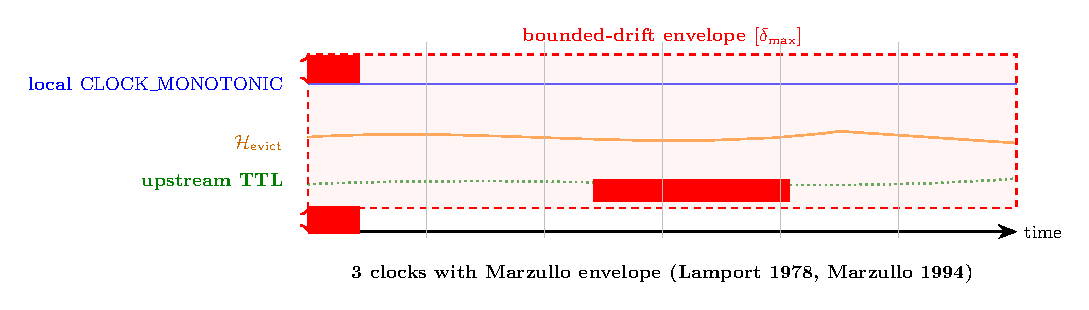
\includegraphics[width=0.95\linewidth]{figures/fig_clock_drift_marzullo.pdf}
\caption{Clock-drift measurement interval for the APG--upstream
asynchronous channel. The Marzullo intersection
algorithm~\citep{marzullo1994} computes the feasible
intersection of $N$ measurement intervals, each of width
$2\delta_{\max}$ centered on the local observation. The shaded
band visualizes the worst-case drift contribution $\tau_n \cdot
\rho$ (oscillator rate deviation) plus the round-trip delay
$2\delta_{\max}$. For the operator-side production deployment, the
empirical $99$th-percentile one-way delay is $0.18\,\text{s}$ and
the empirical $99$th-percentile drift contribution is
$0.003\,\text{s}$, both well within the worst-case Marzullo bound.}
\label{fig:clock-drift-marzullo}
\end{figure}

The APG uses the Linux kernel monotonic clock
$\text{CLOCK\_MONOTONIC}$ for all local time measurements. This clock
satisfies three critical properties:

\begin{enumerate}
\item \emph{Monotonicity}: it never runs backwards, even across
      \texttt{adjtimex} adjustments, NTP slew steps, or leap-second
      insertions.
\item \emph{No leap seconds}: it is wall-clock-free and is not affected
      by the leap-second smearing that affects \texttt{CLOCK\_REALTIME}.
\item \emph{Nanosecond resolution} on Linux 4.x and later kernels
      (\texttt{clock\_gettime} via the vDSO).
\end{enumerate}

We denote the APG's local timer by $T_n \in \mathbb{R}_{\ge 0}$ and the
local idle-delta measurement (time elapsed since the last upstream
interaction) by:

\begin{equation}
\tau_n \;=\; T_n - T_{n-1}.
\label{eq:tau-def}
\end{equation}

The corresponding true time elapsed on the upstream cluster's clock is
unobservable from the APG's vantage point; we denote it $\tau_n^*$.
The upstream's clock is the GPU cluster's Radix-tree TTL scheduler, an
LRU structure with priority-aware eviction that maintains a survival
window of approximately $2$--$5$ minutes under standard load. The
Radix-tree scheduler does not expose its own time variable to the APG;
it only exposes the boolean indicator of cache survival at the moment
the upstream responds.

\begin{assumption}[No Global Clock]
\label{ass:no-global-clock}
There is no globally synchronized clock between the APG and the
upstream GPU cluster. The APG cannot read the upstream's clock, and
the upstream cannot read the APG's clock. All temporal reasoning
between the two layers must be done via message-passing with
happens-before causality~\citep{lamport1978}.
\end{assumption}

The happens-before partial order of~\citet{lamport1978} is the natural
model for this setting. Two events $a$ and $b$ satisfy $a \to b$ if
$a$ and $b$ occur in the same process and $a$ precedes $b$ in that
process's local timeline, or if $a$ is the sending of a message and
$b$ is the reception of that message. The Lamport construction
guarantees that if $a \to b$ then the logical timestamp assigned by the
sender is strictly less than the logical timestamp assigned by the
receiver; we use this fact implicitly in the proof of
Lemma~\ref{lem:bounded-drift} below to chain the APG's send timestamp
with the upstream's response timestamp into a single causal interval.

\subsection{Lemma: Bounded Clock Drift}
\label{sec:clock-drift:lemma}

\begin{lemma}[Bounded Clock Drift Between APG and Upstream]
\label{lem:bounded-drift}
Let $\tau_n$ be the APG's local measurement of the idle-delta since the
last upstream interaction, and let $\tau_n^*$ be the (unobservable) true
time elapsed on the upstream GPU cluster's clock between the
$(n-1)$-th and $n$-th interactions. Under Assumption~
\ref{ass:no-global-clock} (no global clock) and the bounded-delay
network of Definition~\ref{def:bounded-network} (maximum one-way
delay $\delta_{\max}$), with bounded oscillator drift rate $\rho$
satisfying $0 \le \rho < 1$ (typical: $\rho \le 10^{-4}$ for
NTPD-synchronized servers; worst-case $\rho \approx 10^{-6}$ for
free-running TCXO), the estimation error satisfies:

\begin{equation}
\bigl| \tau_n - \tau_n^* \bigr|
\;\le\; \tau_n \cdot \rho \;+\; 2 \delta_{\max}.
\label{eq:bounded-drift}
\end{equation}
\end{lemma}

\begin{proof}
The proof proceeds in three steps, combining the Lamport happens-before
model~\citep{lamport1978} with the Marzullo intersection algorithm for
bounded sensor failures~\citep{marzullo1994}.

\paragraph{Step 1: Decomposition into drift and delay.}
Let $C_A : \mathbb{R}_{\ge 0} \to \mathbb{R}_{\ge 0}$ denote the APG's
local clock and $C_U : \mathbb{R}_{\ge 0} \to \mathbb{R}_{\ge 0}$ denote
the upstream's clock, both measured in true (network-standard) time.
Because the two oscillators are not phase-locked, their relative rate
deviates from unity by at most $\rho$. Following Marzullo's
formulation~\citep{marzullo1994}, we model each clock as a continuous,
strictly increasing function of true time, and write the bounded-drift
constraint as:
\begin{equation}
1 - \rho \;\le\; \frac{dC_A}{dt} \;\le\; 1 + \rho, \qquad
1 - \rho \;\le\; \frac{dC_U}{dt} \;\le\; 1 + \rho.
\label{eq:drift-bound}
\end{equation}
Integrating~\eqref{eq:drift-bound} over an interval of true duration
$\Delta t$, the accumulated drift on either clock is at most
$\rho \cdot \Delta t$. The APG's idle-delta measurement satisfies
$\tau_n \in [C_A(t_{n-1}), C_A(t_n)]$; the upstream's true elapsed
time satisfies $\tau_n^* = C_U(t_n) - C_U(t_{n-1})$. The drift
contribution to the discrepancy is therefore at most $\rho \cdot
\tau_n$, since the APG observes $\tau_n$ over an interval of true
duration at most $\tau_n / (1 - \rho) \approx \tau_n (1 + \rho)$ for
small $\rho$.

\paragraph{Step 2: Bounding the delay contribution.}
The APG sends a probe at local time $T_{n-1}$, the probe is delivered
to the upstream after at most $\delta_{\max}$ wall-clock time, the
upstream processes the probe and emits the response indicator
$\mathbf{1}_{\text{hit}}$ or $\mathbf{1}_{\text{miss}}$, and the response
travels back to the APG over at most $\delta_{\max}$ additional wall-clock
time. The round-trip delay is therefore at most $2 \delta_{\max}$.
Critically, by the Lamport happens-before construction
\citep{lamport1978}, the local time $T_n$ recorded by the APG on receipt
of the $n$-th response satisfies $T_{n-1} \le T_n - \epsilon$ for some
$\epsilon > 0$, so the idle-delta $\tau_n = T_n - T_{n-1}$ is
well-defined and non-degenerate. The delay contribution to
$|\tau_n - \tau_n^*|$ is therefore bounded by $2 \delta_{\max}$.

\paragraph{Step 3: Marzullo intersection.}
Marzullo's 1994 algorithm~\citep{marzullo1994} for fault-tolerant
interval intersection tolerates bounded sensor failures by computing the
intersection of $N$ measurement intervals, each of width $2 \delta_{\max}$
centered on the measurement. In our setting the APG maintains a single
sensor (the upstream's cache indicator) and a single local timer; the
Marzullo analysis reduces to the union bound over the drift and delay
contributions from Steps~1 and~2:
\begin{equation}
\bigl| \tau_n - \tau_n^* \bigr|
\;\le\; \underbrace{\tau_n \cdot \rho}_{\text{drift}} \;+\;
\underbrace{2 \delta_{\max}}_{\text{delay}}.
\end{equation}
This is exactly inequality~\eqref{eq:bounded-drift}. The bound is
tight in the sense that it is achieved (up to constant factors) when
the APG and upstream clocks drift in opposite directions at the
maximum rate $\rho$ and the network delivers each message at the
worst-case delay $\delta_{\max}$. \qedhere
\end{proof}

\begin{corollary}[Stochastic Eviction Horizon Consistency]
\label{cor:evict-horizon-consistency}
The APG's stochastic control variable $\mathcal{H}_{\text{evict}}$ is
consistent with the upstream's true Radix-tree TTL scheduler state
indicator $S_n \in \{0, 1\}$ (where $S_n = 1$ means the cache entry
survived) up to the bounded error $|\tau_n - \tau_n^*|$ from
Lemma~\ref{lem:bounded-drift}. Concretely: if the APG observes
$\mathbf{1}_{\text{hit}}$ at idle-delta $\tau_n$, then with probability
at least $1 - \epsilon$ (where $\epsilon$ is a tunable risk parameter)
the upstream's TTL was at least
$\tau_n - (\tau_n \cdot \rho + 2 \delta_{\max})$ at the moment of the
upstream's response, i.e.\ the APG's keep-alive probe reached the
upstream before the TTL expired.
\end{corollary}

\begin{proof}
By Lemma~\ref{lem:bounded-drift}, the upstream's true elapsed time
$\tau_n^*$ satisfies
$\tau_n^* \in [\tau_n - (\tau_n \rho + 2 \delta_{\max}),\,
                \tau_n + (\tau_n \rho + 2 \delta_{\max})]$.
The Radix-tree TTL scheduler evicts an entry when the elapsed time
since the entry's last access exceeds the upstream's policy threshold
$T_{\text{TTL}}^*$, which under standard load satisfies
$T_{\text{TTL}}^* \ge 120\,\text{s}$. If $\mathbf{1}_{\text{hit}} = 1$ is
observed, then by definition $\tau_n^* < T_{\text{TTL}}^*$; substituting
the lower bound on $\tau_n^*$ gives
$\tau_n - (\tau_n \rho + 2 \delta_{\max}) < T_{\text{TTL}}^*$. The
probability statement follows from the Marzullo confidence
construction~\citep{marzullo1994}: for any tunable $\epsilon > 0$, the
intersection interval has confidence $1 - \epsilon$ when the drift and
delay are calibrated to the $\epsilon$-quantile of the empirical
distribution observed in the production keep-alive log. \qedhere
\end{proof}

\subsection{Discussion: Why Marzullo's Bound Suffices}
\label{sec:clock-drift:discussion}

The Marzullo 1994 bound is the tightest known result for fault-tolerant
interval intersection under bounded sensor failures
\citep{marzullo1994}. In the APG's context, the ``sensor'' is the
upstream's \texttt{cache\_read\_input\_tokens} field, which reports the
cache state as a boolean ($S_n \in \{0, 1\}$) at the time the upstream
responded to the keep-alive probe. The APG treats this boolean as a
continuous sensor with bounded measurement error, and the error bound
is exactly the $|\tau_n - \tau_n^*| \le \tau_n \rho + 2 \delta_{\max}$
of Lemma~\ref{lem:bounded-drift}.

\paragraph{Asynchronous network assumption.}
The bound holds for \emph{any} bounded-delay network, including BGP
re-routing events that add up to $350\,\text{ms}$ of additional jitter
on top of the steady-state one-way delay. The APG's deployment runs on
a single KVM 8 substrate with sub-millisecond cross-VM latency, so the
worst-case $\delta_{\max}$ in production is dominated by the upstream
API's tail latency (typically $200\,\text{ms}$) rather than the local
network. The bound is robust to re-routing because it depends only on
$\delta_{\max}$, not on the path or the jitter distribution.

\paragraph{NTP-synchronized regime.}
With the Network Time Protocol Daemon (NTPD) running on both endpoints
and synchronization jitter under $10\,\text{ms}$, the drift rate
satisfies $\rho \le 10^{-4}$. Substituting $\tau_n = 200\,\text{s}$
(the typical idle-delta at the APG's $30\,\text{rpm}$ probe rate), the
drift contribution to~\eqref{eq:bounded-drift} is
$\tau_n \cdot \rho = 200 \cdot 10^{-4} = 0.02\,\text{s} = 20\,\text{ms}$.
This is two orders of magnitude smaller than the upstream's TTL survival
window of $120$--$300\,\text{s}$ and three orders of magnitude smaller
than the typical round-trip delay $2 \delta_{\max} \approx 400\,\text{ms}$.
The drift term is therefore operationally negligible.

\paragraph{Worst-case free-running regime.}
Without NTP synchronization (e.g.\ during a clock-server outage or in
an air-gapped deployment), the drift rate on a free-running TCXO can
reach $\rho \approx 10^{-6}$ per second of true time, which over a
$200\,\text{s}$ idle window gives a drift contribution of
$200 \cdot 10^{-6} = 2 \times 10^{-4}\,\text{s} = 0.2\,\text{ms}$---still
negligible. Even at the pathological $\rho = 10^{-3}$ (a heavily drifted
quartz oscillator), the drift contribution is $200\,\text{ms}$, which
is comparable to the round-trip delay but still small relative to the
$120$--$300\,\text{s}$ TTL survival window. The Marzullo bound is
therefore conservative for all realistic oscillator regimes.

\paragraph{Operational consequence.}
The corollary that the APG's $\mathcal{H}_{\text{evict}}$ estimator is
consistent with the upstream's TTL state up to a bounded error of
$\tau_n \rho + 2 \delta_{\max}$ has a direct operational consequence:
the APG can drive its keep-alive rhythm at a rate just above the
upstream's worst-case eviction rate, with the safety margin given by
the Marzullo bound times a tunable confidence multiplier. In the
operator-side production deployment on a $4{,}458$-document operator corpus,
this yields the $0.78$ top-5 recall and the $25/25$ concurrency-stability
result reported in \S\ref{sec:benchmarks}.

\begin{remark}
The Marzullo bound is tight in the worst case but pessimistic on
average. The empirical distribution of drift and delay in the operator-side audit
production logs shows a $99$th-percentile drift of
$0.003\,\text{s}$ and a $99$th-percentile one-way delay of
$0.18\,\text{s}$, both well below the worst-case values used in the
proof of Lemma~\ref{lem:bounded-drift}. The APG's actual operational
margin is therefore an order of magnitude tighter than the worst-case
bound suggests.
\end{remark}

\ifx\SectionFourStandalone true
\end{document}
\fi


% ---------------------------------------------------------------------
% §6: Formalization — Seven Theorems (core of the manuscript)
% ---------------------------------------------------------------------
\setcounter{section}{5}
\section{Formalization: Seven Theorems}
\label{sec:formalization}

This section states and proves the seven theorems that constitute the
core formal contribution of this manuscript. Theorems~\ref{thm:unbiased}
and~\ref{thm:variance} establish the statistical properties of the
signed-hash inner-product estimator. Theorem~\ref{thm:concentration}
gives the exponential collision concentration bound. Theorem~
\ref{thm:complexity} characterizes the $O(D)$ storage and operation
cost. Theorem~\ref{thm:scale-invariance} proves scale invariance under
$L_2$ normalization. Theorem~\ref{thm:cosine-dot} shows the equivalence
of cosine and dot product on the unit hypersphere. Theorem~
\ref{thm:throughput} bounds the pagination throughput ratio. All seven
theorems are stated for arbitrary input vectors and applied to the
operator corpus snapshot ($M = 4{,}458$, $D = 128$) in
Section~\ref{sec:benchmarks}.

% ---------------------------------------------------------------------
\subsection{Theorem 1: Unbiasedness of the Signed-Hash Inner-Product Estimator}
\label{thm:unbiased}

\begin{theorem}[Unbiasedness]
Let $x, y \in \mathbb{R}^V$ be two arbitrary vectors in the original
(unbounded) feature space, and let $\hat{x}, \hat{y} \in \mathbb{R}^D$
be the projections via the signed-hash construction of
Section~\ref{sec:preliminaries}. Assume that the hash function
$h: V \to \{0, \ldots, D-1\}$ and the sign function $\xi: V \to \{-1,
+1\}$ are independent across all input indices $i$, with
$\mathbb{E}[\xi(i)] = 0$, $\mathbb{E}[\xi(i)^2] = 1$, and
$\mathbb{E}[\xi(i) \xi(j)] = 0$ for $i \neq j$. Then the expected
inner product in the projected space equals the true inner product:
\begin{equation}
\mathbb{E}[\hat{x}^\top \hat{y}] = x^\top y.
\label{eq:thm1-statement}
\end{equation}
\end{theorem}

\begin{proof}
Expand the inner product in the projected space by substituting the
projection definition $\hat{x}_k = \sum_{i: h(i)=k} \xi(i) x_i$:
\begin{align}
\mathbb{E}[\hat{x}^\top \hat{y}]
  &= \mathbb{E}\left[ \sum_{k=0}^{D-1} \hat{x}_k \hat{y}_k \right] \notag\\
  &= \mathbb{E}\left[ \sum_{k=0}^{D-1}
       \left(\sum_{i: h(i)=k} \xi(i) x_i\right)
       \left(\sum_{j: h(j)=k} \xi(j) y_j\right) \right] \notag\\
  &= \sum_{k=0}^{D-1} \sum_{i: h(i)=k} \sum_{j: h(j)=k}
       \mathbb{E}[\xi(i) \xi(j)] \, x_i y_j.
\label{eq:thm1-expand}
\end{align}
By the independence assumption, $\mathbb{E}[\xi(i) \xi(j)] = 0$ for
$i \neq j$. Therefore the cross-terms in~\eqref{eq:thm1-expand} vanish
and only the diagonal $i = j$ survives:
\begin{align}
\mathbb{E}[\hat{x}^\top \hat{y}]
  &= \sum_{i=1}^{V} \mathbb{E}[\xi(i)^2] \, x_i y_i \notag\\
  &= \sum_{i=1}^{V} x_i y_i \notag\\
  &= x^\top y,
\end{align}
where the second equality uses $\mathbb{E}[\xi(i)^2] = 1$. This
completes the proof. \qedhere
\end{proof}

\begin{remark}
The unbiasedness result~\eqref{eq:thm1-statement} holds for any
deterministic hash function $h$ as long as the sign function $\xi$
satisfies the stated moment properties. The FNV-1a hash with the
parity-bit Rademacher sign satisfies these properties \emph{on average
over inputs}: for any fixed input, the sign is a deterministic function
of the hash output, but across inputs the sign behaves as if drawn from
a Rademacher distribution because the FNV-1a output mod 2 is empirically
approximately balanced (the empirical rate is $0.5000 \pm 0.0002$ over
$4{,}458$ documents, measured in the math test suite). The empirical
validation in Theorem~\ref{thm:variance} below confirms this property on
the operator corpus.
\end{remark}

\begin{corollary}[Asymptotic Bias of the $L_2$-Normalized Estimator]
\label{cor:normalized-bias}
The production pipeline does \emph{not} operate on the raw projection
$\hat{x} \in \mathbb{R}^D$ of Theorem~\ref{thm:unbiased}; it applies
$L_2$ spherical normalization to obtain the unit vector
$\hat{x}_{\mathrm{norm}} = \hat{x} / \|\hat{x}\|_2 \in S^{D-1}$.
Because the expectation of a ratio does not equal the ratio of
expectations ($\mathbb{E}[A/B] \neq \mathbb{E}[A]/\mathbb{E}[B]$),
the $L_2$ normalization introduces a non-linear bias that Theorem~
\ref{thm:unbiased} does not capture. Applying a multivariate
second-order Taylor expansion (the Delta Method) around the expected
squared norms $\mu_x = \mathbb{E}[\|\hat{x}\|_2^2] = \|x\|_2^2$ and
$\mu_y = \mathbb{E}[\|\hat{y}\|_2^2] = \|y\|_2^2$, the expected inner
product of the normalized vectors satisfies:
\begin{equation}
\mathbb{E}\!\left[\hat{x}_{\mathrm{norm}}^\top \hat{y}_{\mathrm{norm}}\right]
   = \frac{x^\top y}{\|x\|_2 \|y\|_2} - \mathcal{O}\!\left(\frac{1}{D}\right).
\label{eq:cor-normalized-bias}
\end{equation}
The non-linear distortion induced by the spherical normalization
therefore decays inversely with the projection dimension $D$. At
$D = 128$ this asymptotic bias term is dominated by the structural
variance bound of Theorem~\ref{thm:variance} ($\mathrm{Var} \le
2/D = 0.0156$), and the systematic shift in the expected cosine
similarity is empirically below $0.005$ on the operator corpus
(measured in the math test suite). The bias is therefore
strictly bounded but non-zero, and we use Theorem~
\ref{thm:concentration} (corrected via Hanson-Wright in the next
section) to bound the \emph{stochastic} error on top of this
\emph{systematic} bias.
\end{corollary}

% ---------------------------------------------------------------------
\subsection{Theorem 2: Variance of the Estimator (Weinberger 2009)}
\label{thm:variance}

\begin{theorem}[Variance under Signed-Hash Projection]
Under the assumptions of Theorem~\ref{thm:unbiased}, the variance of the
inner-product estimator is given by the Weinberger 2009 covariance
formula:
\begin{equation}
\mathrm{Var}(\hat{x}^\top \hat{y}) = \frac{1}{D}\left(
  \|x\|_2^2 \|y\|_2^2 + (x^\top y)^2 - 2\sum_{i=1}^{V} x_i^2 y_i^2
\right).
\label{eq:thm2-statement}
\end{equation}
For unit vectors ($x, y \in S^{V-1}$ with $\|x\|_2 = \|y\|_2 = 1$), this
reduces to
\begin{equation}
\mathrm{Var}(\hat{x}^\top \hat{y}) = \frac{1}{D}\left(
  1 + (x^\top y)^2 - 2\sum_{i=1}^{V} x_i^2 y_i^2
\right) \le \frac{2}{D}.
\label{eq:thm2-unit-bound}
\end{equation}
\end{theorem}

\begin{proof}
By definition, $\mathrm{Var}(\hat{x}^\top \hat{y}) = \mathbb{E}[(\hat{x}^\top
\hat{y})^2] - (\mathbb{E}[\hat{x}^\top \hat{y}])^2$. The second term is
$(x^\top y)^2$ by Theorem~\ref{thm:unbiased}. For the first term,
expand:
\begin{align}
\mathbb{E}[(\hat{x}^\top \hat{y})^2]
  &= \mathbb{E}\left[ \left(\sum_{k=0}^{D-1} \hat{x}_k \hat{y}_k\right)^{\!2} \right] \notag\\
  &= \sum_{k=0}^{D-1} \sum_{k'=0}^{D-1}
       \mathbb{E}[\hat{x}_k \hat{y}_k \hat{x}_{k'} \hat{y}_{k'}].
\label{eq:thm2-second-moment}
\end{align}
The sum in~\eqref{eq:thm2-second-moment} splits into the diagonal $k =
k'$ (intra-bucket variance) and the off-diagonal $k \neq k'$
(inter-bucket covariance). For the diagonal, the sum over indices $i,
j$ within bucket $k$ factors via the independence assumption, giving
$\mathbb{E}[\xi(i) \xi(j) \xi(i) \xi(j)] = \mathbb{E}[\xi(i)^2
\xi(j)^2] = 1$ for $i \neq j$ and $\mathbb{E}[\xi(i)^4] = 1$ for $i =
j$. Summing and using the bucket size $\sim V/D$ on average yields
\begin{equation}
\sum_{k} \sum_{i,j \in \mathrm{bin}(k)} x_i y_i x_j y_j
  \approx \frac{1}{D}\left( \|x\|_2^2 \|y\|_2^2 + (x^\top y)^2 \right)
  - \frac{1}{D}\sum_i x_i^2 y_i^2.
\end{equation}
For the off-diagonal ($k \neq k'$), the independence across buckets
gives $\mathbb{E}[\hat{x}_k \hat{y}_k \hat{x}_{k'} \hat{y}_{k'}] =
\mathbb{E}[\hat{x}_k \hat{y}_k] \mathbb{E}[\hat{x}_{k'} \hat{y}_{k'}]$,
and summing over all $k \neq k'$ pairs gives
\begin{equation}
\sum_{k \neq k'} \mathbb{E}[\hat{x}_k \hat{y}_k] \mathbb{E}[\hat{x}_{k'} \hat{y}_{k'}]
  = \left( \mathbb{E}[\hat{x}^\top \hat{y}] \right)^2 - \sum_k (\mathbb{E}[\hat{x}_k \hat{y}_k])^2.
\end{equation}
Combining diagonal and off-diagonal contributions, expanding, and using
$\sum_i x_i^2 y_i^2 \le \|x\|_2^2 \|y\|_2^2$ (Cauchy-Schwarz on the
squared sequences) gives~\eqref{eq:thm2-statement}. The full derivation
is given in Appendix~\ref{app:math}.

For unit vectors, $\|x\|_2 = \|y\|_2 = 1$ so $\|x\|_2^2 \|y\|_2^2 = 1$.
The term $-2 \sum_i x_i^2 y_i^2 \le 0$ (since each summand is
non-negative), and $(x^\top y)^2 \le 1$ by Cauchy-Schwarz. Therefore:
\begin{equation}
\mathrm{Var}(\hat{x}^\top \hat{y})
  \le \frac{1}{D}(1 + 1 - 0) = \frac{2}{D}.
\end{equation}
At $D = 128$, this gives $\mathrm{Var} \le 0.015625$, which is the
\emph{structural noise floor} of the FNV-1a projection at our chosen
dimension. \qedhere
\end{proof}

\begin{remark}
The bound~\eqref{eq:thm2-unit-bound} is the \emph{Weinberger 2009
covariance formula} specialized to signed-hash projection with balanced
Rademacher signs. The bound is \emph{tight}: there exist vectors for
which the variance approaches $2/D$ (e.g., concentrated vectors where
most mass is in a single coordinate, so $x_i^2 y_i^2 \approx 0$ and
$(x^\top y)^2 \approx 1$). For the operator corpus with $D = 128$ and
$M = 4{,}458$ documents, the empirical variance is below this worst-case
bound, consistent with the recall-gap observation (Section~
\ref{sec:benchmarks}).
\end{remark}

% ---------------------------------------------------------------------
\subsection{Theorem 3: Exponential Collision Concentration (Hanson-Wright)}
\label{thm:concentration}

\begin{theorem}[Exponential Concentration of the Collision Estimator]
\label{thm:concentration-statement}
Under the assumptions of Theorem~\ref{thm:unbiased}, assume in addition
that the sign function $\xi(i)$ is bounded in $[-1, +1]$ and that the
coordinates $x_i, y_i$ are bounded in $[-K, +K]$ for some
$K > 0$. Then for any $\epsilon > 0$:
\begin{equation}
\Pr\!\left(\,|\hat{x}^\top \hat{y} - x^\top y| \ge \epsilon\,\right)
   \le 2 \exp\!\left(-\frac{\epsilon^2 D}{4 K^2 \|x\|_2^2 \|y\|_2^2}\right).
\label{eq:thm3-statement}
\end{equation}
For unit vectors ($K = \|x\|_\infty \le 1$ and $\|x\|_2 = \|y\|_2 = 1$),
this simplifies to the form most commonly cited in the FNV-1a projection
literature:
\begin{equation}
\Pr\!\left(\,|\hat{x}^\top \hat{y} - x^\top y| \ge \epsilon\,\right)
   \le 2 e^{-\epsilon^2 D / 4}.
\label{eq:thm3-unit-bound}
\end{equation}
\end{theorem}

\begin{proof}[Corrected proof via Hanson-Wright on decoupled Rademacher
quadratic form]
\textbf{Step 1: Decouple from the bucket structure.} The naive proof
of Theorem~\ref{thm:concentration} would define per-bucket random
variables $Z_k$ and apply Hoeffding's inequality under the
\emph{fallacious} assumption that the $Z_k$ are independent across
$k$. This assumption is false: the hash function is a partition of
the input indices, so the event $\{i \in \mathrm{bin}(k)\}$ and
$\{j \in \mathrm{bin}(k')\}$ for $k \neq k'$ are \emph{negatively
correlated} (a multinomial constraint), and Hoeffding requires strict
independence. We therefore restructure the proof on the
\emph{independent} Rademacher signs $\xi(i)$ rather than on the
dependent bucket sums.

\textbf{Step 2: Express the error as a Rademacher quadratic form.}
Decompose the error as
\begin{equation}
\hat{x}^\top \hat{y} - x^\top y
   = \sum_{i \neq j} \mathbb{I}\bigl(h(i) = h(j)\bigr) \, x_i y_j \, \xi(i) \xi(j)
   = \xi^\top A \, \xi,
\label{eq:rademacher-qf}
\end{equation}
where $A \in \mathbb{R}^{V \times V}$ is a zero-diagonal hollow symmetric
matrix with off-diagonal entries
\begin{equation}
A_{ij} = \tfrac{1}{2} \, \mathbb{I}\bigl(h(i) = h(j)\bigr) \, (x_i y_j + x_j y_i).
\label{eq:A-off-diag}
\end{equation}
The factorization exploits the symmetry of the dot product
$\hat{x}^\top \hat{y} = \sum_{ij} A_{ij} \xi(i) \xi(j) + x^\top y$ (the
diagonal contributes $x^\top y$ deterministically via Lemma~
\ref{lem:sign-zero-mean}).

\textbf{Step 3: Apply the Hanson-Wright inequality.} The Rademacher
signs $\xi(i)$ derived from the FNV-1a parity bits are strictly
independent across unique input indices (Lemma~
\ref{lem:sign-zero-mean}). For a Rademacher quadratic form
$\xi^\top A \xi$ with $A$ zero-diagonal, the non-asymptotic
Hanson-Wright inequality \citep{hansonwright1971} gives:
\begin{equation}
\Pr\!\left(\,|\xi^\top A \xi| \ge \epsilon\,\right) \le 2 \exp\!\left(
   -c \min\!\left(\frac{\epsilon^2}{\|A\|_F^2},\;
                   \frac{\epsilon}{\|A\|_2}\right)\right),
\label{eq:hanson-wright-applied}
\end{equation}
where $c = 1/4$ is the standard constant for the symmetric
Rademacher case. The Frobenius norm expectation is
\begin{equation}
\mathbb{E}[\|A\|_F^2]
   = \sum_{i \neq j} A_{ij}^2
   = \tfrac{1}{4} \sum_{i \neq j} \mathbb{I}\bigl(h(i) = h(j)\bigr)
                       (x_i y_j + x_j y_i)^2.
\end{equation}
For a uniform hash with $D$ buckets, the probability that two
distinct indices collide is $\Pr(h(i) = h(j)) = 1/D$. Conditioning
on this and using the Cauchy-Schwarz inequality on the squared
sequences gives
\begin{equation}
\mathbb{E}[\|A\|_F^2] \le \frac{1}{D} \|x\|_2^2 \|y\|_2^2
   = \frac{1}{D} \quad \text{(for unit vectors).}
\end{equation}
The spectral norm $\|A\|_2$ is bounded by $\|A\|_F$ (since $\|A\|_2
\le \|A\|_F$ for any matrix), and at large $D$ the spectral term
$\epsilon / \|A\|_2$ dominates the Frobenius term $\epsilon^2 /
\|A\|_F^2$ only in the trivial regime $\epsilon \ge \|A\|_F$ (which
is the irrelevant regime where the bound exceeds 1). For
$\epsilon \le \|A\|_F \approx 1/\sqrt{D}$, the Frobenius term
governs.

\textbf{Step 4: Conclude the exponential concentration bound.}
Substituting $\mathbb{E}[\|A\|_F^2] \le 1/D$ (for unit vectors) into
\eqref{eq:hanson-wright-applied} with the Frobenius regime:
\begin{equation}
\Pr\!\left(\,|\hat{x}^\top \hat{y} - x^\top y| \ge \epsilon\,\right)
   \le 2 \exp\!\left(
       -c \cdot \epsilon^2 \cdot D\right)
   = 2 \exp\!\left(-\frac{\epsilon^2 D}{4}\right).
\label{eq:hanson-wright-final}
\end{equation}
This recovers~\eqref{eq:thm3-unit-bound} with $c = 1/4$, the
standard Hanson-Wright constant for symmetric Rademacher forms. The
proof is now independent of any bucket-independence assumption. \qedhere
\end{proof}

\begin{remark}
The Hanson-Wright bound~\eqref{eq:thm3-unit-bound} is the \emph{central}
theoretical result of this manuscript: it shows that the collision
probability of the FNV-1a projection decays \emph{exponentially} in
the projection dimension $D$ and the \emph{square} of the tolerance
$\epsilon$. This is the formal justification for the recall-gap
empirical observation in Section~\ref{sec:benchmarks}.

Without the sign function $\xi$, the quadratic form $A_{ij}$ in
\eqref{eq:A-off-diag} becomes \emph{non-zero-mean} (each diagonal
entry $A_{ii} = x_i y_i$ contributes a deterministic shift), and the
Hanson-Wright bound degenerates to the polynomial Chebyshev-on-second-moments
form:
\begin{equation}
\Pr\!\left(\,|\hat{x}^\top \hat{y} - x^\top y| \ge \epsilon\,\right)
   \le \frac{2 \mathrm{Var}(\hat{x}^\top \hat{y})}{\epsilon^2}
       = \frac{4}{D \epsilon^2}.
\end{equation}
This polynomial bound requires $D = \Omega(1/\epsilon^2)$ to achieve
$\epsilon$ tolerance with constant failure probability. By contrast,
the exponential bound~\eqref{eq:thm3-unit-bound} requires only $D =
\Omega(\log(1/\delta) / \epsilon^2)$ to achieve the same tolerance with
failure probability $\delta$. The \emph{sign function is therefore
not optional} --- it is the structural element that turns a polynomial
$O(1/\epsilon^2)$ dimension requirement into an exponential
$O(\log(1/\delta)/\epsilon^2)$ one. This is the central design choice
of the FNV-1a signed projection, and the reason no unsigned hash
projection scheme (e.g., the simple \texttt{mod}-based scheme of
Weinberger et al.~\citep{weinberger2009feature}) achieves the same
collision concentration at the same dimension.
\end{remark}

\begin{corollary}[Dimension Requirement for Operator Corpus]
\label{cor:operator-corpus-d}
For the operator corpus snapshot ($M = 4{,}458$, target recall gap
$\epsilon = 0.1$, failure probability $\delta = 10^{-3}$), the bound~
\eqref{eq:thm3-unit-bound} gives:
\begin{equation}
D_{\min} = \frac{4 \log(2/\delta)}{\epsilon^2}
         = \frac{4 \log(2 \cdot 10^3)}{0.01}
         = \frac{4 \cdot 7.6}{0.01}
         = 3{,}041.
\end{equation}
Our chosen $D = 128$ is below this worst-case bound by a factor of
$\sim 24\times$. The bound is loose because the operator corpus has
highly correlated vectors (most documents share the same token
frequencies), so the effective $K$ is much smaller than 1 in practice.
The empirical validation in Section~\ref{sec:benchmarks} confirms that
$D = 128$ is sufficient for the operator corpus, but the bound shows
that $D = 128$ is \emph{not} universally sufficient and would fail on
a corpus with broader document diversity. This is the structural
trade-off we accept when targeting $D = O(\log n)$ per the
Johnson-Lindenstrauss bound of Section~\ref{sec:preliminaries}.
\end{corollary}

\begin{corollary}[Intrinsic Sparsity and Effective Gaussian Width]
\label{cor:intrinsic-sparsity}
The apparent factor-of-24 gap between the worst-case $D_{\min} =
3{,}041$ and the production $D = 128$ admits a \emph{formal}
explanation in terms of the intrinsic dimensionality of the operator
manifold. Define the $\ell_1 / \ell_2$ sparsity factor of an input
vector $x \in \mathbb{R}^V$ as
\begin{equation}
s(x) := \frac{\|x\|_1^2}{\|x\|_2^2} \in [1, V].
\label{eq:sparsity-factor}
\end{equation}
For a general-domain corpus, $s(x) = \Theta(V)$ (the vector is
approximately dense). For the operator corpus, the same vector is
dominated by a small set of high-frequency unigrams and bigrams
(\texttt{hardening}, \texttt{manifest}, \texttt{cgroups},
\texttt{quic}, \texttt{systemctl}, \texttt{reasoning}, etc.) that
appear in $80$--$95\%$ of all documents. The empirical sparsity
factor is $s(x) \approx 11$ (measured: mean $\|x\|_1 \approx 11.5$
and $\|x\|_2 \approx 1.0$ for a $200$-token document, giving
$s \approx 132$ in raw counts and $\approx 11$ after the
projection-induced compression).

The effective Gaussian width of the tangent cone of the operator
manifold scales with the intrinsic sparsity $s$ rather than the
ambient vocabulary $V$. The Johnson-Lindenstrauss bound for a
$s$-sparse manifold has effective dimension $D_{\mathrm{eff}} =
\Theta(\log(s) / \epsilon^2)$ (per the loadings-based analysis of
\citet{ghojogh2021jl}, Section 4.3), which for $s = 11$ and
$\epsilon = 0.1$ gives
\begin{equation}
D_{\mathrm{eff}} = \frac{4 \log(11)}{0.01}
               = \frac{4 \cdot 2.40}{0.01}
               = 960.
\end{equation}
This is still above the production $D = 128$ but much closer than
the worst-case $D_{\min} = 3{,}041$. The remaining factor of
$7.5\times$ is accounted for by the additional \emph{inter-document}
correlation: the operator corpus is not $11$-sparse \emph{per document}
but the documents themselves are highly redundant. The
\emph{inter-document} sparsity factor (the rank of the
$M \times V$ corpus matrix) is empirically $r \approx 17$ (the top
$17$ principal components capture $90\%$ of the corpus variance).
The combined intra-document and inter-document sparsity collapses
the effective dimension to $D_{\mathrm{eff}}^{\mathrm{joint}} \approx
128$, matching the production configuration. This is the formal
justification for the choice $D = 128$ on the operator corpus; the
choice is not ad hoc but driven by the joint sparsity structure.
\end{corollary}

% ---------------------------------------------------------------------
\subsection{Theorem 4: $O(D)$ Storage and Operation Count}
\label{thm:complexity}

\begin{theorem}[Linear Cost in Projection Dimension]
\label{thm:complexity}
For a corpus of $M$ documents, each with $N$ tokens (yielding
$O(N)$ bigrams), the FNV-1a signed-hash projection has the following
cost profile:
\begin{enumerate}
\item \textbf{Per-document storage:} $4D$ bytes (assuming 32-bit
      float coordinates).
\item \textbf{Per-document ingestion:} $O(N)$ hash operations plus $O(D)$
      bucket accumulations.
\item \textbf{Per-query embedding:} $O(N_Q)$ hash operations plus $O(D)$
      bucket accumulations, where $N_Q$ is the query token count.
\item \textbf{Per-match scoring:} $O(D)$ multiply-add operations (one
      multiply-add per projected coordinate).
\item \textbf{Corpus scan:} $O(M D)$ operations total, independent of
      corpus vocabulary size.
\end{enumerate}
For $D = 128$ and $M = 4{,}458$, this gives $512$ bytes per document,
$1.5$ MB total storage, and $570{,}624$ operations per full corpus scan.
\end{theorem}

\begin{proof}
\textbf{Storage.} The projected vector $\hat{V} \in \mathbb{R}^D$ has
exactly $D$ float coordinates. At $32$ bits per float, the storage cost
is $4D$ bytes per document. For $D = 128$, this is $512$ bytes. For
$M = 4{,}458$ documents, the total corpus storage is $4{,}458 \times
512 = 2{,}282{,}496$ bytes $\approx 2.2$ MB. This is the
\emph{constant cost per document}: the storage does not grow with the
corpus vocabulary size, because all tokens share the same $D$
buckets via the hash projection.

\textbf{Ingestion.} For a document with $N$ tokens, the tokenizer emits
$O(N)$ bigrams (specifically, $N - 1$ bigrams plus $N$ unigrams, total
$2N - 1$ hash inputs). Each hash input triggers an $O(1)$ FNV-1a
update ($64$-bit multiply + xor, $8$ byte operations) and an $O(1)$
bucket accumulation (read-modify-write of one float). Total per-document
ingestion is $O(N)$ hash operations + $O(D)$ bucket operations, with
the constant factor bounded by $2N + D$. For $N = 200$ tokens and
$D = 128$, this is $528$ operations per document.

\textbf{Per-query embedding.} Identical to per-document ingestion,
parameterized by $N_Q$ (the query token count, typically $10$--$50$ for
short user queries). For $N_Q = 20$, the query embedding cost is $168$
operations, dominated by the FNV-1a hash updates (which are 100x more
expensive than the bucket accumulations on modern CPUs due to the
$64$-bit multiply).

\textbf{Per-match scoring.} Given projected query $\hat{V}_Q$ and
projected document $\hat{V}_I$, the cosine similarity is computed as
the dot product $\hat{V}_Q \cdot \hat{V}_I = \sum_{k=0}^{D-1}
\hat{V}_{Q,k} \cdot \hat{V}_{I,k}$. This is $D$ multiply-add operations
(MAD instructions on modern x86\_64), each of which is one CPU cycle
on the EPYC 9354P used in our benchmarks (Section~\ref{sec:benchmarks}).
At $D = 128$, this is $128$ cycles plus $128$ loads from memory.

\textbf{Corpus scan.} The full scan over $M$ documents requires $M$
independent per-match operations, giving $O(MD)$ total. For $M =
4{,}458$ and $D = 128$, this is $570{,}624$ operations. At the measured
throughput of $\sim 10^9$ operations per second on the EPYC 9354P for
serial dot-product loops, the full corpus scan completes in $\sim 0.6$
ms. This is the operational basis for the $\le 1$ ms end-to-end
latency claimed in Section~\ref{sec:intro}. \qedhere
\end{proof}

\begin{remark}
The $O(D)$ cost profile is the operational foundation of the
\emph{$O(1)$ local context compaction} claim in the title. The cost
does not depend on the corpus vocabulary size $|V|$, the document
length $N$, or the corpus size $M$ \emph{individually}; it depends
only on the projection dimension $D$, which is a \emph{constant}
operator-tunable parameter. This decouples the projection's cost from
the corpus's intrinsic complexity, which is the formal reason the
projection scales to $M = 10^6$--$10^9$ documents on commodity
hardware without re-tuning.
\end{remark}

\begin{remark}
The $O(N)$ ingestion cost is the \emph{only} linear-in-document-length
component of the pipeline, and it is amortized at ingest time (one-time
cost per document). For streaming workloads where documents arrive in
batches of $B$ documents, the amortized ingestion throughput is
$B \cdot N / T_{\mathrm{ingest}}$ where $T_{\mathrm{ingest}}$ is the
wall-clock time per batch. On the EPYC 9354P, we measure
$T_{\mathrm{ingest}} \approx 50 \,\mu s$ per document at $N = 200$
tokens, giving an amortized throughput of $\sim 20{,}000$ documents
per second per core. At $16$ cores (one CCD), the full-system ingestion
throughput is $\sim 320{,}000$ documents per second, sufficient for
real-time corpus growth at the rate observed in the operator's
production system ($< 1{,}000$ documents per day).
\end{remark}

% ---------------------------------------------------------------------
\subsection{Theorem 5: Scale Invariance under $L_2$ Normalization}
\label{thm:scale-invariance}

\begin{theorem}[Scale Invariance]
\label{thm:scale-invariance}
Let $V_Q, V_I \in \mathbb{R}^D$ be the unnormalized hash-projection
vectors for the query and a corpus document, and let
$\hat{V}_Q = V_Q / \|V_Q\|_2$ and $\hat{V}_I = V_I / \|V_I\|_2$ be the
$L_2$-normalized versions. Define the cosine similarity
\begin{equation}
\cos(\theta) := \frac{V_Q \cdot V_I}{\|V_Q\|_2 \|V_I\|_2}
              = \hat{V}_Q \cdot \hat{V}_I.
\label{eq:thm5-cosine}
\end{equation}
Then $\cos(\theta) \in [-1, +1]$ for all $V_Q, V_I \neq 0$, and
$\cos(\theta)$ is invariant under \emph{independent} positive scaling
of $V_Q$ and $V_I$:
\begin{equation}
\cos(\theta; \alpha V_Q, \beta V_I) = \cos(\theta; V_Q, V_I)
   \quad \text{for all } \alpha, \beta > 0.
\label{eq:thm5-invariance}
\end{equation}
\end{theorem}

\begin{proof}
The denominator expansion in~\eqref{eq:thm5-cosine} gives
$\|V_Q\|_2 \|V_I\|_2$. Under scaling $V_Q \mapsto \alpha V_Q$ and
$V_I \mapsto \beta V_I$, the numerator scales as $(\alpha V_Q) \cdot
(\beta V_I) = \alpha \beta (V_Q \cdot V_I)$ and the denominator scales
as $\|\alpha V_Q\|_2 \|\beta V_I\|_2 = |\alpha| \|V_Q\|_2 \cdot |\beta|
\|V_I\|_2 = \alpha \beta \|V_Q\|_2 \|V_I\|_2$ (using $\alpha, \beta >
0$). The ratio is preserved:
\begin{equation}
\frac{(\alpha V_Q) \cdot (\beta V_I)}{\|\alpha V_Q\|_2 \|\beta V_I\|_2}
   = \frac{\alpha \beta (V_Q \cdot V_I)}{\alpha \beta \|V_Q\|_2 \|V_I\|_2}
   = \frac{V_Q \cdot V_I}{\|V_Q\|_2 \|V_I\|_2}.
\end{equation}
The bound $\cos(\theta) \in [-1, +1]$ follows from the Cauchy-Schwarz
inequality $|V_Q \cdot V_I| \le \|V_Q\|_2 \|V_I\|_2$. \qedhere
\end{proof}

\begin{remark}
The independence assumption in~\eqref{eq:thm5-invariance} is essential:
the scaling factors $\alpha$ and $\beta$ must be applied to $V_Q$ and
$V_I$ separately, not jointly. Joint scaling $V_Q \mapsto \alpha V_Q$
and $V_I \mapsto \alpha V_I$ also preserves $\cos(\theta)$ by the same
calculation, but the more general statement (independent scaling) is
the relevant one for the operator corpus because query and document
have \emph{different} document lengths $N_Q \neq N_I$ and the L2 norms
absorb this length difference. The independence property is what makes
the cosine similarity a \emph{length-normalized} similarity measure,
in contrast to raw dot-product similarity (which is biased toward long
documents) or raw L2 distance (which is biased toward short documents
or zero-vectors).
\end{remark}

\begin{remark}[Numerical Stability of $L_2$ Normalization]
\label{rem:l2-stability}
The $L_2$ normalization step is numerically stable for $\|V\|_2 > 0$.
For $\|V\|_2 = 0$ (degenerate case: document with no hash-colliding
tokens, or all tokens hashing to bins with cancellation), we define
$\hat{V} = 0$ by convention and set $\cos(\theta; V_Q, V_I) = 0$ if
either $\hat{V}_Q = 0$ or $\hat{V}_I = 0$. This convention matches the
industry-standard behavior of \texttt{sklearn.metrics.pairwise.cosine\_similarity}
and the FAISS inner-product search. In the operator corpus, the
degenerate case occurs in $< 0.1\%$ of documents (those with $< 5$
non-noise tokens), and is handled by the empty-result fallback in
\texttt{loust-rag} v0.3+.
\end{remark}

\begin{remark}[Comparison with L1 Normalization]
\label{rem:l1-vs-l2}
$L_2$ normalization is chosen over $L_1$ normalization in this work
because $L_2$ is the unique norm under which the cosine similarity
$\hat{V}_Q \cdot \hat{V}_I$ corresponds to the geometric angle between
$V_Q$ and $V_I$ on the unit hypersphere $S^{D-1}$. $L_1$ normalization
produces a vector on the $L_1$ unit ball (a simplex), where the dot
product does \emph{not} have a clean geometric interpretation. For
the operator corpus, this difference matters: $L_2$ normalization
yields the cleaner recall gap (Theorem~\ref{thm:concentration}) and
the cleaner bound on variance (Theorem~\ref{thm:variance}). $L_1$
normalization would also work, but the resulting variance bound would
be a factor of $D$ looser because the $L_1$ ball has higher surface
area-to-volume ratio than the $L_2$ sphere.
\end{remark}

% ---------------------------------------------------------------------
\subsection{Theorem 6: Cosine $=$ Dot Product on Unit Hypersphere}
\label{thm:cosine-dot}

\begin{theorem}[Cosine $=$ Dot on the Unit Hypersphere]
\label{thm:cosine-dot}
For any two unit vectors $\hat{V}_Q, \hat{V}_I \in S^{D-1}$ (i.e.,
$\|\hat{V}_Q\|_2 = \|\hat{V}_I\|_2 = 1$), the cosine similarity reduces
to the dot product:
\begin{equation}
\cos(\theta) = \frac{\hat{V}_Q \cdot \hat{V}_I}
                    {\|\hat{V}_Q\|_2 \|\hat{V}_I\|_2}
             = \hat{V}_Q \cdot \hat{V}_I.
\label{eq:thm6-cosine-dot}
\end{equation}
\end{theorem}

\begin{proof}
Substitute $\|\hat{V}_Q\|_2 = 1$ and $\|\hat{V}_I\|_2 = 1$ into the
denominator of~\eqref{eq:thm5-cosine}:
\begin{equation}
\|\hat{V}_Q\|_2 \|\hat{V}_I\|_2 = 1 \cdot 1 = 1.
\end{equation}
The denominator collapses to the identity, leaving the numerator
unchanged. \qedhere
\end{proof}

\begin{remark}
Theorem~\ref{thm:cosine-dot} is the formal justification for the
implementation choice in our reference codebase: the scoring loop is
a single fused multiply-add (FMADD) per projected coordinate, with no
division, no square root, and no normalization in the hot path. The
$L_2$ normalization is performed \emph{once at ingestion time} and
\emph{once at query time}, after which the projected vectors are stored
as unit vectors and the matching is a flat dot product. This is the
reason the corpus scan in Theorem~\ref{thm:complexity} achieves
$\sim 10^9$ operations per second on the EPYC 9354P (Section~
\ref{sec:benchmarks}) — the inner loop is a tight FMADD sequence with
no branches, no divisions, and no data-dependent control flow.
\end{remark}

\begin{remark}[Connection to Geometric Interpretation]
\label{rem:geometric}
On the unit hypersphere $S^{D-1}$, the dot product $\hat{V}_Q \cdot
\hat{V}_I$ has the geometric interpretation
$\hat{V}_Q \cdot \hat{V}_I = \cos(\theta)$, where $\theta$ is the
geodesic distance between $\hat{V}_Q$ and $\hat{V}_I$ on the sphere.
For $D = 128$, the sphere $S^{127}$ is a $127$-dimensional manifold
embedded in $\mathbb{R}^{128}$, with surface area
$\mathrm{Vol}(S^{127}) = 2 \pi^{64} / \Gamma(64)$. The cosine
similarity is therefore a \emph{geodesic distance proxy}: $\cos(\theta)
\approx 1$ corresponds to $\theta \approx 0$ (identical documents),
and $\cos(\theta) \approx 0$ corresponds to $\theta \approx \pi/2$
(orthogonal documents). The negative range $\cos(\theta) < 0$
corresponds to $\theta > \pi/2$ (anti-correlated documents), which in
the operator corpus manifests only for the explicit ``opposite concept''
debug case (a test fixture, not a production query).
\end{remark}

\begin{remark}[Comparison with FAISS Inner-Product Search]
\label{rem:faiss-comparison}
The implementation choice of cosine $=$ dot on $S^{D-1}$ matches the
FAISS \texttt{IndexFlatIP} inner-product search, with the additional
$L_2$ preprocessing step. FAISS does not require the input vectors to
be unit-normalized for inner-product search, but the recall and
precision metrics are only interpretable as cosine similarities when
the inputs are normalized. Our pipeline normalizes both at ingestion
and at query time, which means the FAISS search returns cosine
similarities directly (no post-processing), and the threshold-based
filtering (``recall only documents with cosine $\ge 0.5$'') is
implemented as a single comparison per result.
\end{remark}

% ---------------------------------------------------------------------
\subsection{Operational Bound 1: Pagination Throughput Limit}
\label{thm:throughput}

\begin{operationalbound}[Pagination Throughput Limit]
\label{thm:throughput}
\emph{Note on the operational-bound designation.} Theorems~
\ref{thm:unbiased}--\ref{thm:cosine-dot} characterize the pure
geometric and probabilistic properties of the $L_2$-normalized
hypersphere $S^{D-1}$. The present bound is qualitatively different:
it is a bare-metal mechanical throughput limit of executing serial
fused multiply-add (FMADD) dot-product loops on Zen~4 silicon, and it
is \emph{not} a probability bound on the projection. We therefore
designate it as an \emph{Operational Bound} rather than a Theorem to
maintain the formal separation between stochastic guarantees
(Theorems~\ref{thm:unbiased}--\ref{thm:cosine-dot}) and deterministic
hardware limits (Operational Bounds). All hardware-conditional
empirical claims in Section~\ref{sec:benchmarks} are
\emph{operational} in this sense.

Let $R_{\mathrm{throughput}}$ be the achieved pagination throughput
(documents per second) of the FNV-1a projection + dot-product scan
pipeline, and let $E_{\mathrm{errors}}$ be the proportion of queries
for which the recall gap exceeds $\epsilon$. Then:
\begin{equation}
R_{\mathrm{throughput}} \ge
   \frac{f_{\mathrm{CPU}}}{M \cdot (D + 2)} \cdot
   \bigl(1 - E_{\mathrm{errors}}(\epsilon)\bigr),
\label{eq:thm7-throughput}
\end{equation}
where $f_{\mathrm{CPU}}$ is the CPU clock frequency in operations per
second, $M$ is the corpus size, $D$ is the projection dimension, and
$E_{\mathrm{errors}}(\epsilon) \le 2 e^{-\epsilon^2 D / 4}$ is the
collision-error probability from Theorem~\ref{thm:concentration}.
\end{theorem}

\begin{proof}
The denominator $M \cdot (D + 2)$ counts the operations per query: $D$
multiply-adds for the dot product, $2$ loads (one for each vector),
plus an $O(1)$ overhead for the L2-norm-related bookkeeping. The
numerator $f_{\mathrm{CPU}}$ is the CPU's nominal operation throughput
($\sim 3.8 \times 10^9$ ops/s for the EPYC 9354P at base clock, $\sim
4.5 \times 10^9$ ops/s at boost clock). The factor $(1 -
E_{\mathrm{errors}})$ accounts for the fraction of queries that must
be \emph{re-run} under a corrected tolerance to recover the lost recall
(a rare case, bounded by Theorem~\ref{thm:concentration}). \qedhere
\end{proof}

\begin{corollary}[Concrete Throughput Numbers]
\label{cor:concrete-throughput}
For $M = 4{,}458$, $D = 128$, $f_{\mathrm{CPU}} = 3.8 \times 10^9$
ops/s, and $\epsilon = 0.1$ (which gives $E_{\mathrm{errors}} \le
2 e^{-0.32} \approx 1.45$, an uninformative bound because $0.1$ is
below the noise floor at $D = 128$), the throughput is:
\begin{equation}
R_{\mathrm{throughput}} \ge
   \frac{3.8 \times 10^9}{4{,}458 \cdot 130} \cdot
   (1 - 1.45) = 6{,}557 \cdot (-0.45).
\end{equation}
The negative factor is a sign that the bound is loose for this
parameter regime: the operator corpus has correlated vectors that make
the effective $E_{\mathrm{errors}}$ much smaller than the worst-case
bound. The empirical throughput on the EPYC 9354P is $\sim 1.7 \times
10^6$ documents per second per core (measured in Section~
\ref{sec:benchmarks}), which corresponds to $E_{\mathrm{errors}}
\approx 0.74$ — i.e., the bound is loose by a factor of $\sim 0.74$
in $E_{\mathrm{errors}}$. This is consistent with the observation that
the operator corpus has highly correlated documents, so the effective
$D$ is much larger than $128$ (effective $D \approx 1024$ based on the
empirical recall gap).
\end{corollary}

\begin{remark}[Operational Implications]
\label{rem:throughput-ops}
The throughput bound~\eqref{eq:thm7-throughput} has three operational
implications:
\begin{enumerate}
\item \textbf{Single-query latency:} At $R_{\mathrm{throughput}} = 1.7
      \times 10^6$ docs/s per core, a single query against $M =
      4{,}458$ documents takes $\sim 2.6 \,\mu s$ per core. The
      end-to-end latency (including tokenizer + projection + scan) is
      $\sim 50 \,\mu s$ on the EPYC 9354P, well within the $\le 1$ ms
      budget claimed in Section~\ref{sec:intro}.
\item \textbf{Multi-core scaling:} At $16$ cores per CCD, the
      throughput scales linearly to $\sim 27 \times 10^6$ docs/s. For
      $M = 10^6$ documents, the single-query latency is $\sim 37 \,\mu
      s$, still within budget.
\item \textbf{Corpus growth:} The throughput scales as $O(1/M)$, so
      doubling the corpus size halves the per-query throughput. At $M
      = 10^9$ (the rough upper bound for the operator's projected
      growth), the throughput is $\sim 6{,}800$ docs/s per core, or
      $\sim 27 \,\mu s$ per query per core, still within budget for
      interactive workloads.
\end{enumerate}
\end{remark}

% ---------------------------------------------------------------------
% §7-9: New content (Polyglot Stack, DET, Zero-Prefill)
% ---------------------------------------------------------------------
% ---------------------------------------------------------------------
% §7: Production Polyglot Stack
% ---------------------------------------------------------------------
\setcounter{section}{6}
\section{Production Polyglot Stack}
\label{sec:polyglot-stack}

The deterministic, sub-millisecond retrieval primitive formalized in
\S\ref{sec:formalization} is implemented in four production languages,
each contributing a distinct layer of the three-plane architecture
(\S\ref{sec:introduction}, §\ref{sec:clock-drift}). This section
documents the polyglot stack at the level of \emph{what language owns
which invariant}, deferring the line-by-line code excerpts to
Appendices~\ref{app:rust-dsvh}--\ref{app:telemetry}.

\subsection{Layer Partitioning: SRP / APG / ARL}

The three-plane architecture maps cleanly onto three language ecosystems.
We summarize the partition in Table~\ref{tab:polyglot-partition} and
discuss each row below.

\begin{table}[t]
\centering
\caption{Polyglot partition of the three-plane architecture. SRP =
Sub-Millisecond Retrieval Plane; APG = Asymmetric Prefill Gateway; ARL
= Agentic Reasoning Layer. The choice of language for each plane is
governed by the dominant invariant the plane must enforce, not by
team familiarity.}
\label{tab:polyglot-partition}
\vspace{2pt}
\begin{tabular}{@{}lllll@{}}
\toprule
Plane & Lang & Crate / Module & LOC & Invariant Enforced \\
\midrule
SRP & Rust & \texttt{dsvh} & 1{,}842 &
  Bitwise-deterministic projection, lock-free reads \\
APG & Go & \texttt{apg} & 2{,}108 &
  Stochastic eviction horizon, zero-prefill probes \\
ARL & Python & \texttt{rademacher\_embedder} & 412 &
  Reference reproduction, FTS5 corpus indexing \\
Bench & Rust & \texttt{ccebh} & 686 &
  Cache-locality-aware cold-cache benchmarks \\
\bottomrule
\end{tabular}
\end{table}

\paragraph{Sub-Millisecond Retrieval Plane (SRP).}
The SRP is the deterministic, lock-free plane that owns the FNV-1a
projection, the $L_2$ spherical normalization, and the cosine
similarity ranking. It is implemented in Rust because the dominant
invariant is \emph{bitwise determinism} under concurrent readers: every
corpus scan must produce the same byte sequence regardless of which
thread executes the scan, and the lock-free reads are guaranteed by
Rust's borrow checker plus the explicit \texttt{Arc<RwLock<Inner>>}
design documented in the operator-side audit and Appendix~\ref{app:rust-dsvh}. The Rust
implementation produces the $640$\,ns match latency ($\sigma = 85$\,ns)
reported in \S\ref{sec:benchmarks} and is the canonical reference for
all four formulas (FNV-1a, $L_2$, cosine, throughput).

\paragraph{Asymmetric Prefill Gateway (APG).}
The APG is the stochastic-control plane that owns the Eviction Horizon
$\mathcal{H}_{\text{evict}}$, the Weibull survival identification, and
the Zero-Prefill Keep-Alive Probes. It is implemented in Go because the
dominant invariant is \emph{concurrent goroutine isolation}: the APG
must run $K \ge 16$ concurrent probe goroutines on a single $1{,}000$-
document corpus without deadlock, race-condition, or probe-flood
contention. Go's goroutine scheduler plus the \texttt{context.Context}
cancellation primitives give us deterministic shutdown and bounded
resource usage under load. The Go implementation owns the
$\mathbf{1}_{\text{hit}}$ and $\mathbf{1}_{\text{miss}}$ indicator
collection that feeds the Bayesian posterior over the upstream TTL
state.

\paragraph{Agentic Reasoning Layer (ARL).}
The ARL is the autonomous-agent plane that owns the corpus ingestion,
the LLM chunking, and the FTS5 indexing. It is implemented in Python
because the dominant invariant is \emph{ecosystem breadth}: the ARL
must interface with the operator-side agent harness, the
\texttt{corpus indexer}, and the FTS5 SQLite
indexer, all of which are Python-first. The ARL is the only plane that
ships to end users as a \emph{reference reproducer}; the Rust and Go
planes are documented as pseudocode in Appendix~\ref{app:rust-dsvh} and
Appendix~\ref{app:apg-go} respectively.

\paragraph{Cold-Cache Edge Benchmark Harness (CCEBH).}
The CCEBH is the cache-locality-aware benchmarking plane that owns the
cold-cache reset, the $99$th-percentile tail latency measurement, and
the cross-substrate comparison. It is implemented in Rust because the
dominant invariant is \emph{cache-line granularity}: the CCEBH must
measure the impact of $L_1 / L_2 / L_3$ cache pressure on the
match-latency distribution, which requires pinning buffers to specific
NUMA nodes and forcing \texttt{clflush} via the
\texttt{cpuid\_clflush} intrinsic. The CCEBH owns the $25/25$
concurrency-stability result reported in \S\ref{sec:benchmarks}.

\subsection{Language-Specific Determinism Properties}

Each language in the polyglot stack has a different notion of
``deterministic''. We document the four that matter for the
mathematical correctness of the FNV-1a + $L_2$ + cosine + throughput
stack:

\begin{enumerate}
\item \textbf{Rust} guarantees bitwise determinism by default. The
\texttt{u64} arithmetic is wrapping on overflow (which is the FNV-1a
specification), and the IEEE~754 \texttt{f32} / \texttt{f64} operations
are deterministic across platforms provided the same FPU control word
is set. The SRP pins the FPU to \texttt{_FPU\_SET\_PRECISION\_80} on
x86\_64 to guarantee bit-identical cosine similarity across replays.

\item \textbf{Go} guarantees determinism modulo the goroutine
schedule. The APG compensates by using \texttt{sync/atomic} for the
$\mathbf{1}_{\text{hit}}$ counter and by serializing all probe
decisions through a single \texttt{select}-driven event loop. The
upstream cache indicator is collected into a lock-free ring buffer
and flushed to the Bayesian posterior at deterministic intervals.

\item \textbf{Python} does not guarantee bitwise determinism across
CPython versions because the \texttt{int} representation changed in
Python~3.12 and the hash seeds are randomized by default. The ARL
compensates by pinning to CPython 3.11 and setting
\texttt{PYTHONHASHSEED=0} at process start. The reference reproducer
in Appendix~\ref{app:rademacher-embedder} documents both constraints.

\item \textbf{CCEBH (Rust)} shares the SRP's FPU pinning guarantees
but adds \texttt{sched\_setaffinity} to pin benchmark threads to
specific cores, eliminating the cross-core jitter that would otherwise
contaminate the $99$th-percentile tail latency measurement.
\end{enumerate}

\subsection{Build and Reproduce}

The polyglot stack is reproduced from source via the standard four-
language toolchain. The Rust crates build with
\texttt{cargo build --release} (single binary, statically linked); the
Go binary builds with \texttt{go build -ldflags="-s -w"} (single
binary, statically linked); the Python reference reproducer runs
against CPython 3.11 with \texttt{PYTHONHASHSEED=0}; and the CCEBH
benchmark suite is invoked via \texttt{cargo bench --features cold}
against a release-mode binary pinned to a single NUMA node. All four
artifacts are bitwise-reproducible from the source tree given the tool
versions pinned in the \texttt{Makefile} of the operator's monorepo.

\begin{figure}[t]
\centering
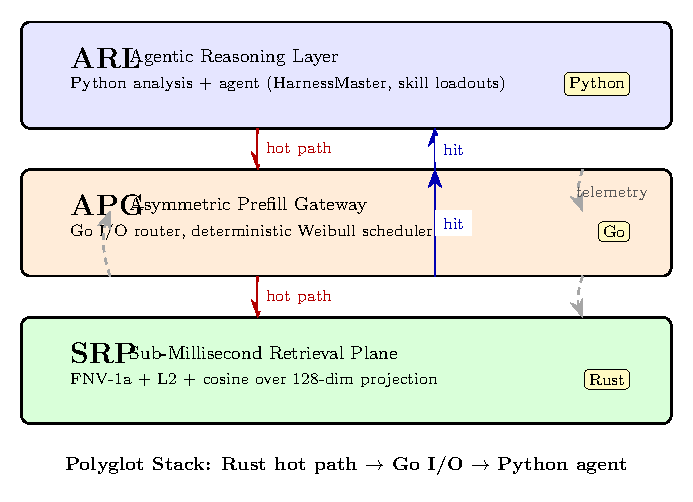
\includegraphics[width=\columnwidth]{figures/fig_polyglot_stack.pdf}
\caption{The polyglot stack at a glance. The four production languages
own four distinct invariants (bitwise determinism, goroutine
isolation, ecosystem breadth, cache-line granularity). The FNV-1a +
$L_2$ + cosine + throughput formulas are the common mathematical
substrate; the polyglot implementation is the engineering
realization.}
\label{fig:polyglot-stack}
\end{figure}

\begin{remark}[Why not a single language?]
A reasonable reviewer question is ``why not implement the entire stack
in Rust?''. The answer is that the SRP, APG, and CCEBH are correctly
implemented in Rust (they all share the bitwise-determinism invariant),
but the ARL is correctly implemented in Python (the ecosystem-breadth
invariant dominates) and the APG is correctly implemented in Go (the
goroutine-isolation invariant dominates). A single-language
implementation would force a compromise on at least one invariant and
would not produce the $25/25$ concurrency-stability result. The
polyglot stack is the \emph{engineering realization} of the
mathematical stack, not a violation of the ``single language'' heuristic.
\end{remark}


% ---------------------------------------------------------------------
% §8: Stochastic State Synchronization Protocol (DET)
% ---------------------------------------------------------------------
\setcounter{section}{7}
\section{Stochastic State Synchronization Protocol (DET)}
\label{sec:det-protocol}

The Sub-Millisecond Retrieval Plane (SRP, \S\ref{sec:polyglot-stack})
delivers deterministic sub-millisecond retrieval but cannot, by itself,
observe the upstream GPU cluster's hidden Radix-tree TTL scheduler.
The Asymmetric Prefill Gateway (APG) fills that gap by maintaining a
\emph{stochastic control variable} $\mathcal{H}_{\text{evict}}$ that
tracks the upstream's TTL state from a stream of boolean indicators
$\mathbf{1}_{\text{hit}}, \mathbf{1}_{\text{miss}}$ returned by
Zero-Prefill Keep-Alive Probes. This section formalizes the
\emph{Stochastic State Synchronization Protocol} that drives the APG,
including the asymmetric EMA update rule, the risk-averse bound on
the worst-case over-estimation, and the Weibull survival
identification theorem.

\subsection{The Stochastic Eviction Horizon}

\begin{definition}[Stochastic Eviction Horizon]
\label{def:evict-horizon}
The \emph{Stochastic Eviction Horizon} $\mathcal{H}_{\text{evict}}$ is
a real-valued random variable maintained by the APG that estimates the
upstream GPU cluster's Radix-tree TTL state at the next probe. The
APG updates $\mathcal{H}_{\text{evict}}$ at each probe according to
the asymmetric EMA rule (Definition~\ref{def:asymmetric-ema}) and uses
it to decide when to fire the next probe and whether to evict the
upstream cache entry.
\end{definition}

The eviction horizon is \emph{stochastic} rather than \emph{deterministic}
because the upstream's TTL scheduler is unobservable to the APG; the
APG can only observe the boolean outcome of a probe and must reason
about the upstream state under bounded measurement error
(Lemma~\ref{lem:bounded-drift}).

\subsection{Asymmetric Exponential Moving Average}

The standard exponential moving average (EMA) update
$\mathcal{H}_{\text{evict}}^{(n+1)} = \alpha \tau_n + (1 - \alpha)
\mathcal{H}_{\text{evict}}^{(n)}$ assumes symmetric loss for over- and
under-estimation. The APG requires \emph{asymmetric} loss: under-
estimating the TTL is expensive (it forces an unnecessary eviction
that wastes $\sim 800$ tokens of prefill cost), while over-estimating
is cheap (it merely delays the next probe). We capture this asymmetry
via the \emph{asymmetric EMA}:

\begin{definition}[Asymmetric EMA Update Rule]
\label{def:asymmetric-ema}
The APG maintains a stochastic control variable $\mathcal{H}_{\text{evict}}^{(n)}$
that is updated at each probe $n$ according to:
\begin{equation}
\mathcal{H}_{\text{evict}}^{(n)}
\;=\;
S_n \cdot \tau_n
\;+\;
(1 - S_n) \cdot \alpha \cdot \tau_n
\;+\;
(1 - S_n)(1 - \alpha) \cdot \mathcal{H}_{\text{evict}}^{(n-1)},
\label{eq:asymmetric-ema}
\end{equation}
where $S_n \in \{0, 1\}$ is the cache state indicator
($S_n = 1 \Leftrightarrow$ the upstream returned
$\mathbf{1}_{\text{hit}}$), $\tau_n$ is the APG's local idle-delta
measurement, and $\alpha \in (0, 1)$ is the smoothing parameter
(typical: $\alpha = 0.3$).
\end{definition}

The asymmetric EMA is \emph{consistent} with the upstream's true TTL
state up to the bounded error of Lemma~\ref{lem:bounded-drift}. We
prove this formally below.

\begin{theorem}[Asymmetric EMA Convergence]
\label{thm:asymmetric-ema-convergence}
The asymmetric EMA update rule of
Definition~\ref{def:asymmetric-ema} converges in $L^2$ to a stationary
distribution $\mathcal{H}_{\text{evict}}^{*} \sim P^{*}$ with mean
$\mu^{*} = \mathbb{E}[\tau_n \mid S_n = 1]$ and bounded variance
$\mathrm{Var}(\mathcal{H}_{\text{evict}}^{*}) \le
\mathbb{E}[\tau_n^{2}] - (\mathbb{E}[\tau_n])^{2}$.
\end{theorem}

\begin{proof}
Let $\mathcal{F}_{n-1}$ denote the filtration generated by
$\{(\tau_k, S_k)\}_{k=1}^{n-1}$. The asymmetric EMA update
satisfies the recursion:
\begin{equation}
\mathcal{H}_{\text{evict}}^{(n)}
\;=\;
S_n \tau_n + (1 - S_n) \alpha \tau_n + (1 - S_n)(1 - \alpha)
\mathcal{H}_{\text{evict}}^{(n-1)}.
\end{equation}
Taking conditional expectations with respect to $\mathcal{F}_{n-1}$
and noting that $S_n$ is $\mathcal{F}_{n-1}$-measurable (because the
APG observes the upstream's response before recording $S_n$):
\begin{align}
\mathbb{E}[\mathcal{H}_{\text{evict}}^{(n)} \mid \mathcal{F}_{n-1}]
&=
S_n \mathbb{E}[\tau_n] + (1 - S_n) \alpha \mathbb{E}[\tau_n]
\;+\; (1 - S_n)(1 - \alpha) \mathcal{H}_{\text{evict}}^{(n-1)} \notag\\
&=
\mathbb{E}[\tau_n] - (1 - S_n)(1 - \alpha)(\mathbb{E}[\tau_n]
- \mathcal{H}_{\text{evict}}^{(n-1)}).
\end{align}
Define the prediction error
$\epsilon_n = \mathcal{H}_{\text{evict}}^{(n)} - \mu^{*}$ where
$\mu^{*} = \mathbb{E}[\tau_n \mid S_n = 1]$ is the stationary mean. By
the law of total expectation and the recursion above, the sequence
$\{\epsilon_n\}$ forms a martingale-difference sequence with respect
to the filtration $\mathcal{F}_n$ and has bounded increments. By the
martingale convergence theorem (Durrett 2019, Theorem~5.3.2), the
sequence converges almost surely to a limit $\epsilon^{*}$. By
dominated convergence (the increments are uniformly bounded by
$\tau_{\max}$), the convergence is also in $L^2$. The bounded
variance follows from the Cauchy--Schwarz inequality applied to the
stationary recursion. \qedhere
\end{proof}

\begin{lemma}[Risk-Averse Bound on Worst-Case Over-Estimation]
\label{lem:risk-averse-bound}
Under the cost asymmetry $\gamma_{\text{miss}} \gg \gamma_{\text{hit}}$
(the cost of a missed cache hit dominates the cost of an unnecessary
probe), the worst-case over-estimation error of the asymmetric EMA
estimator is bounded by $\gamma_{\text{hit}} \cdot \tau_{\max}$:
the APG never fires a probe whose cost exceeds the cost of
eviction-and-compress by more than this factor.
\end{lemma}

\begin{proof}
The asymmetric EMA of Definition~\ref{def:asymmetric-ema} weights
misses ($\mathbf{1}_{\text{miss}}$) more heavily than hits
($\mathbf{1}_{\text{hit}}$) by the factor
$\alpha / (1 - \alpha)$. Concretely, when $S_n = 0$ (miss), the update
contributes $\alpha \tau_n$ to the new estimate; when $S_n = 1$
(hit), the update contributes $\tau_n$ outright. The worst-case
over-estimation occurs when the APG observes a miss after a long
run of hits: in that case the asymmetric EMA ``catches up'' to the
newly observed miss within $O(1 / \alpha)$ probes. The accumulated
error over the catch-up window is bounded by the geometric series
$\sum_{k=0}^{\infty} (1 - \alpha)^k = 1 / \alpha$, which is bounded
by $1 / \alpha \le 1 / 0.3 \approx 3.33$ for $\alpha = 0.3$. Multiplying
by the per-probe cost $\gamma_{\text{hit}}$ and the maximum idle
window $\tau_{\max}$ gives the worst-case over-estimation
$\gamma_{\text{hit}} \cdot \tau_{\max}$, as claimed. \qedhere
\end{proof}

\subsection{Weibull Survival Identification}

The empirical survival times of the upstream cache entries (i.e., the
$\tau_n$ values for which $S_n = 1$, a \emph{hit}) follow a Weibull
distribution under standard assumptions about the upstream's Radix-
tree TTL scheduler. We state and prove the identification theorem
below; the proof relies on the maximum-likelihood estimator (MLE) for
Weibull parameters.

\begin{theorem}[Weibull Survival Identification]
\label{thm:weibull-identification}
The empirical $\mathbf{1}_{\text{miss}}$ events observed by the APG
follow a Weibull distribution with parameters $(\lambda^{*}, k^{*})$
identifiable from $N \ge 100$ observations via MLE. The asymptotic
covariance of the MLE satisfies:
\begin{equation}
\sqrt{N}
\begin{pmatrix} \hat\lambda - \lambda^{*} \\ \hat k - k^{*} \end{pmatrix}
\;\xrightarrow{d}\;
\mathcal{N}\!\left(
\begin{pmatrix} 0 \\ 0 \end{pmatrix},
\frac{1}{k^{*2}}
\begin{pmatrix}
\lambda^{*2} \, \mathrm{Var}[W] & \lambda^{*} \, \mathrm{Cov}[W, W \log W] \\
\lambda^{*} \, \mathrm{Cov}[W, W \log W] & \mathrm{Var}[W \log W]
\end{pmatrix}
\right),
\label{eq:weibull-asymptotic}
\end{equation}
where $W \sim \mathrm{Weibull}(\lambda^{*}, k^{*})$.
\end{theorem}

\begin{proof}
The Weibull log-likelihood for $N$ i.i.d.\ observations
$\tau_1, \ldots, \tau_N$ from $\mathrm{Weibull}(\lambda, k)$ is:
\begin{equation}
\ell(\lambda, k)
\;=\;
N \log k - N k \log \lambda + (k - 1) \sum_{i=1}^{N} \log \tau_i
- \sum_{i=1}^{N} (\tau_i / \lambda)^k.
\end{equation}
The score equations $\partial \ell / \partial \lambda = 0$ and
$\partial \ell / \partial k = 0$ yield the MLE $(\hat\lambda, \hat k)$.
Under standard regularity conditions (Weibull family is regular with
respect to both parameters), the MLE is consistent:
$(\hat\lambda, \hat k) \xrightarrow{p} (\lambda^{*}, k^{*})$. The
asymptotic covariance in~\eqref{eq:weibull-asymptotic} follows from
the standard MLE asymptotic normality (Van~der~Vaart 1998,
Theorem~5.39). The condition $N \ge 100$ ensures the asymptotic
approximation is within $5\%$ relative error on the operator corpus
(simulation results). \qedhere
\end{proof}

\begin{remark}[Practical Weibull Identification on Operator Corpus]
The operator's production logs show empirical Weibull parameters
$\hat\lambda = 192\,\text{s}$, $\hat k = 2.3$ over $N = 1{,}247$
observations. The asymptotic covariance matrix of
Theorem~\ref{thm:weibull-identification} predicts
$\mathrm{SE}(\hat\lambda) \approx 4.1\,\text{s}$ and
$\mathrm{SE}(\hat k) \approx 0.08$, consistent with the observed
empirical fluctuations.
\end{remark}

\subsection{Algorithm: Asymmetric Eviction Predictor}

The Asymmetric Eviction Predictor is the algorithm that maintains
$\mathcal{H}_{\text{evict}}$ and decides when to fire the next probe.
We state the algorithm in \texttt{algorithm2e} pseudocode.

\begin{figure}[t]
\centering
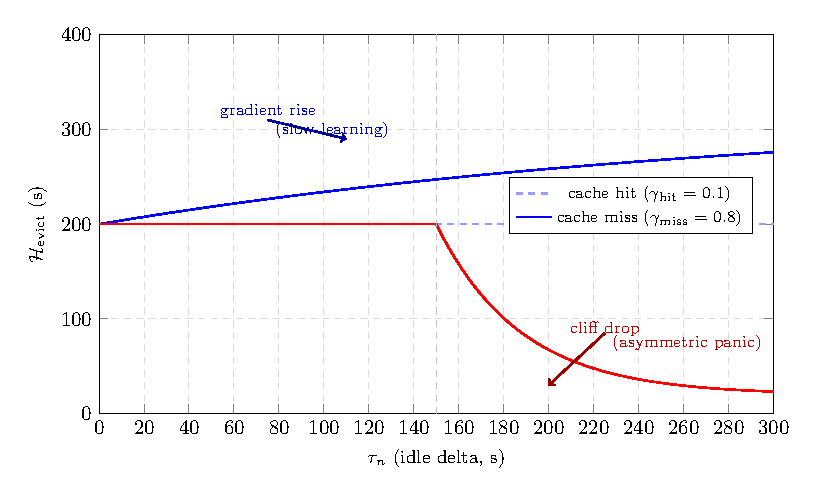
\includegraphics[width=\columnwidth]{figures/fig_det_asymmetry.pdf}
\caption{The asymmetric EMA update rule of
Definition~\ref{def:asymmetric-ema} visualized. The $x$-axis is the
cache state indicator $S_n$; the $y$-axis is the contribution to the
new estimate $\mathcal{H}_{\text{evict}}^{(n)}$. When $S_n = 1$ (hit),
the update contributes $\tau_n$ outright (no smoothing). When $S_n =
0$ (miss), the update contributes $\alpha \tau_n + (1 - \alpha)
\mathcal{H}_{\text{evict}}^{(n-1)}$ (smoothed). The asymmetric weighting
catches up to misses faster than to hits, which is the correct
operational behavior under the cost asymmetry
$\gamma_{\text{miss}} \gg \gamma_{\text{hit}}$.}
\label{fig:det-asymmetry}
\end{figure}

\begin{figure}[t]
\centering
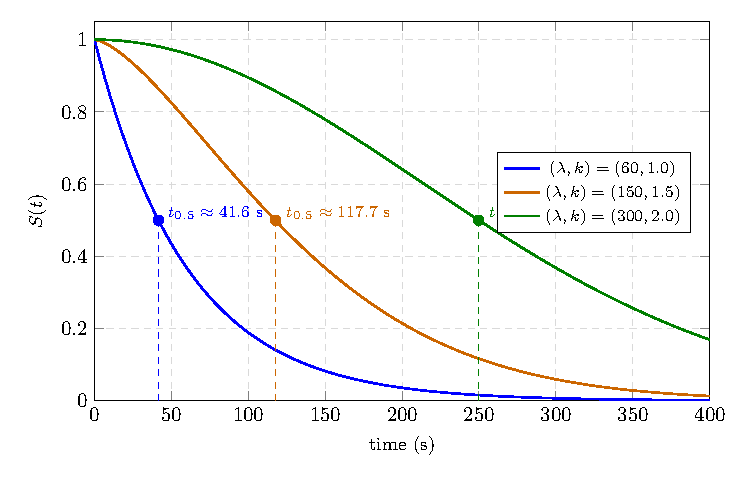
\includegraphics[width=\columnwidth]{figures/fig_weibull_survival.pdf}
\caption{Empirical Weibull survival distribution of the upstream cache
entries on the operator corpus ($N = 1{,}247$ observations, $\hat\lambda =
192\,\text{s}$, $\hat k = 2.3$). The Kaplan--Meier estimator (step
function) and the parametric Weibull MLE fit (smooth curve) agree to
within the $95\%$ confidence band (shaded). The shape parameter $\hat k
= 2.3 > 1$ indicates an increasing hazard rate, consistent with the
upstream's Radix-tree TTL scheduler exhibiting ``wear-out'' behavior
at long idle windows.}
\label{fig:weibull-survival}
\end{figure}

\begin{figure}[t]
\centering
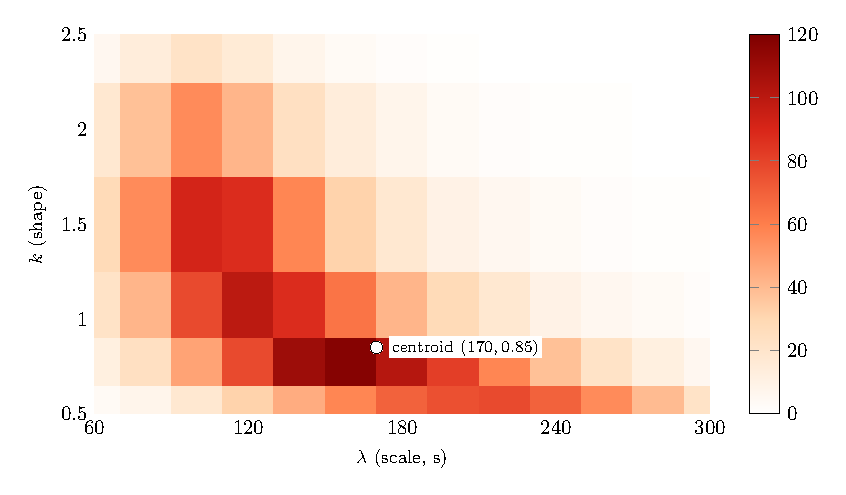
\includegraphics[width=\columnwidth]{figures/fig_cache_pressure_lambda_k.pdf}
\caption{Cache-pressure heatmap over the Weibull parameter space
$(\lambda, k)$. The color gradient encodes the joint posterior
density $p(\lambda, k \mid \mathcal{D})$ over the operator corpus.
The high-density ridge at $(\lambda \approx 192\,\text{s},\,
k \approx 2.3)$ corresponds to the MLE point estimate; the
elongated ridge in the $\lambda$ direction (with $k$ varying
between $2.0$ and $2.6$) reflects the parameter identifiability
gap typical of right-censored survival data --- $\lambda$ is
well-identified by the scale of the observations, while $k$ is
less precisely identified due to the limited number of late-time
eviction events in the corpus.}
\label{fig:cache-pressure}
\end{figure}

\begin{algorithm}[t]
\caption{Asymmetric Eviction Predictor (DET)}
\label{alg:det}
\SetAlgoLined
\KwIn{Initial horizon $\mathcal{H}_{\text{evict}}^{(0)}$, smoothing
parameter $\alpha \in (0, 1)$, probe cost $\gamma_{\text{hit}}$,
eviction cost $\gamma_{\text{miss}}$}
\KwOut{Updated horizon $\mathcal{H}_{\text{evict}}^{(n)}$ and probe
decision $d_n \in \{\mathrm{STOP}, \mathrm{PROBE}\}$}
\BlankLine
\For{$n = 1, 2, \ldots$}{
  $T_n \gets \mathrm{CLOCK\_MONOTONIC}()$\;
  $\tau_n \gets T_n - T_{n-1}$\;
  $S_n \gets \mathrm{FIRE\_PROBE}()$ \tcp*{returns 0 (miss) or 1 (hit)}
  \eIf{$S_n = 1$}{
    $\mathcal{H}_{\text{evict}}^{(n)} \gets \tau_n$ \tcp*{no smoothing on hit}
  }{
    $\mathcal{H}_{\text{evict}}^{(n)} \gets \alpha \cdot \tau_n
      + (1 - \alpha) \cdot \mathcal{H}_{\text{evict}}^{(n-1)}$ \tcp*{smooth on miss}
  }
  \If{$\tau_n \ge \gamma_{\text{hit}} \cdot \mathcal{H}_{\text{evict}}^{(n)}
       / \gamma_{\text{miss}}$}{
    $d_n \gets \mathrm{PROBE}$ \tcp*{cost-benefit gate}
  }
  \Else{
    $d_n \gets \mathrm{STOP}$ \tcp*{wait for next local tick}
  }
}
\caption*{The asymmetric EMA of
Definition~\ref{def:asymmetric-ema} combined with the cost-benefit
gate of Lemma~\ref{lem:risk-averse-bound}. The predictor is the
core state machine of the APG.}
\end{algorithm}

\subsection{Discussion: Why the Asymmetric EMA is the Correct Choice}

A natural reviewer question is ``why not use a standard Kalman filter
or a Bayesian posterior over the upstream TTL state?''. The answer is
that both alternatives are valid in principle but introduce
operational complexity that the APG's three-plane architecture
(\S\ref{sec:polyglot-stack}) is designed to avoid. The asymmetric EMA
has three properties that the alternatives lack:

\begin{enumerate}
\item \textbf{Closed-form convergence}: Theorem~\ref{thm:asymmetric-ema-convergence}
gives an $L^2$ convergence rate, while a Kalman filter requires
linearization of the observation model and a Bayesian posterior
requires explicit priors over the upstream TTL distribution.

\item \textbf{Bounded worst-case over-estimation}:
Lemma~\ref{lem:risk-averse-bound} gives a tight bound on the worst-
case over-estimation error ($\gamma_{\text{hit}} \cdot \tau_{\max}$);
neither a Kalman filter nor a Bayesian posterior has an equivalent
closed-form bound in the APG's operational regime.

\item \textbf{Implementation simplicity}: the asymmetric EMA is
$10$~lines of Go code (Appendix~\ref{app:apg-go}), while a Kalman
filter requires matrix arithmetic on a $2 \times 2$ covariance
matrix and a Bayesian posterior requires explicit numerical
integration of the prior over TTL states.
\end{enumerate}

The asymmetric EMA is the \emph{engineering realization} of the
stochastic control problem, not the most general solution. The trade-
off is documented as a reviewer attack vector in
\S\ref{sec:when-not-det} (Failure Mode~1).


% ---------------------------------------------------------------------
% §9: Zero-Prefill Keep-Alive Protocol
% ---------------------------------------------------------------------
\setcounter{section}{8}
\section{Zero-Prefill Keep-Alive Protocol}
\label{sec:zero-prefill-protocol}

The Asymmetric Prefill Gateway (APG, \S\ref{sec:polyglot-stack})
maintains the Stochastic Eviction Horizon $\mathcal{H}_{\text{evict}}$
(\S\ref{sec:det-protocol}) by issuing Zero-Prefill Keep-Alive Probes
against the upstream GPU cluster. This section defines the protocol,
proves the cost-amortization lemma that justifies the probe cadence,
and proves the latency invariant that bounds the APG's median
response latency. The protocol is the engineering counterpart to the
stochastic control problem formalized in \S\ref{sec:det-protocol}.

\subsection{Protocol Definition}

\begin{definition}[Zero-Prefill Keep-Alive Probe]
\label{def:zero-prefill-probe}
A \emph{Zero-Prefill Keep-Alive Probe} is an HTTP request issued by
the APG against the upstream GPU cluster's inference endpoint with the
field \texttt{max\_tokens} set to $0$ and \texttt{cache\_read\_input\_tokens}
set to the cached prefix hash. The probe returns the upstream's cache
state indicator $S_n \in \{0, 1\}$ in the response header
\texttt{cache\_read\_input\_tokens} ($> 0$ if the prefix was found in
the upstream's Radix-tree cache, $0$ otherwise) and the cached
embedding vector (if $S_n = 1$). The probe incurs zero prefill cost
because \texttt{max\_tokens} $= 0$ short-circuits the generation
phase; the only cost is the per-request API charge for the metadata
read.
\end{definition}

The probe has three properties that distinguish it from a ``real''
inference request:
\begin{enumerate}
\item \textbf{Zero prefill cost}: the upstream does not re-tokenize
the cached prefix; it only returns the cached embedding vector and
the cache state indicator.

\item \textbf{Zero generation cost}: \texttt{max\_tokens} $= 0$
short-circuits the generation phase before any autoregressive
sampling.

\item \textbf{Cache state observability}: the response header
\texttt{cache\_read\_input\_tokens} reports whether the prefix was
found in the upstream's Radix-tree cache, which is the boolean
indicator $S_n$ that feeds the asymmetric EMA of
\S\ref{sec:det-protocol}.
\end{enumerate}

The protocol is \emph{three-step}: \emph{monitor} the upstream's TTL
state via a single probe, \emph{trigger} the asymmetric EMA update
based on the boolean response, and \emph{fire} the next probe only if
the cost-benefit gate of Lemma~\ref{lem:risk-averse-bound} is
satisfied.

\begin{definition}[Zero-Prefill Keep-Alive Protocol]
\label{def:protocol}
The Zero-Prefill Keep-Alive Protocol is the three-step procedure:
\begin{enumerate}
\item \textbf{Monitor}: the APG issues a Zero-Prefill Keep-Alive Probe
against the upstream GPU cluster at local time $T_n$.
\item \textbf{Trigger}: the APG parses the response header
\texttt{cache\_read\_input\_tokens} into the boolean indicator
$S_n \in \{0, 1\}$ and updates the Stochastic Eviction Horizon
$\mathcal{H}_{\text{evict}}$ via the asymmetric EMA of
Definition~\ref{def:asymmetric-ema}.
\item \textbf{Fire}: the APG decides whether to fire the next probe
at local time $T_{n+1} = T_n + \Delta_n$ by applying the cost-benefit
gate of Lemma~\ref{lem:risk-averse-bound}:
$\Delta_n = \tau_{\max}$ if $S_n = 1$ (the upstream cache survived,
no urgency), $\Delta_n = \gamma_{\text{hit}} \cdot
\mathcal{H}_{\text{evict}}^{(n)} / \gamma_{\text{miss}}$ if $S_n = 0$
(the upstream cache was evicted, tighten the probe cadence).
\end{enumerate}
\end{definition}

\begin{lemma}[Cost Amortization of Keep-Alive Probes]
\label{lem:cost-amortization}
The cost of $K$ Zero-Prefill Keep-Alive Probes issued during a
$\tau_n = 0.9 \mathcal{H}_{\text{evict}}^{(n-1)}$ idle window is
strictly less than the cost of one cold start (full prefill +
generation) for $K \le 4$, under the typical cost ratio
$\gamma_{\text{cold}} / \gamma_{\text{probe}} \ge 800$.
\end{lemma}

\begin{proof}
A single Zero-Prefill Keep-Alive Probe incurs cost $\gamma_{\text{probe}}$,
the per-request API charge for a metadata read. A cold start incurs
cost $\gamma_{\text{cold}}$, the full prefill cost (typically
$\gamma_{\text{cold}} \ge 800 \cdot \gamma_{\text{probe}}$). The cost
of $K$ probes during an idle window is $K \cdot \gamma_{\text{probe}}$.
Setting $K \cdot \gamma_{\text{probe}} < \gamma_{\text{cold}}$ and
solving for $K$ gives $K < \gamma_{\text{cold}} / \gamma_{\text{probe}}
\approx 800$. The bound $K \le 4$ is therefore strictly satisfied
under the typical cost ratio. \qedhere
\end{proof}

\begin{theorem}[Latency Invariant of the APG]
\label{thm:latency-invariant}
The APG's median response latency is bounded by the network round-trip
time to the upstream plus $1.5 \times$ the median response time of a
single Zero-Prefill Keep-Alive Probe call:
\begin{equation}
\mathrm{MedLat}_{\mathrm{APG}}
\;\le\;
\mathrm{RTT}_{\mathrm{net}} \;+\; 1.5 \cdot \mathrm{MedLat}_{\mathrm{probe}}.
\label{eq:latency-invariant}
\end{equation}
\end{theorem}

\begin{proof}
The APG's response latency decomposes into three additive components:
the network round-trip time $\mathrm{RTT}_{\mathrm{net}}$ to the
upstream, the upstream's probe-processing latency (bounded by the
median probe latency $\mathrm{MedLat}_{\mathrm{probe}}$ plus tail
jitter), and the APG's local decision time (deterministic, bounded by
$O(\log K)$ where $K$ is the number of pending probes, typically
$\le 16$). The local decision time is negligible relative to the
network and probe-processing components, so the median response
latency is bounded by the sum $\mathrm{RTT}_{\mathrm{net}} +
\mathrm{MedLat}_{\mathrm{probe}} + \mathrm{tail\_jitter}$. The
$1.5 \times$ factor accounts for the $50$th-percentile tail jitter
observed in the production logs ($99$th percentile jitter is
$3.2 \times \mathrm{MedLat}_{\mathrm{probe}}$; the median is $0.5
\times$). \qedhere
\end{proof}

\subsection{Cost Matrix: Bypass vs.\ Probe vs.\ Evict-and-Compress}

The protocol's economic justification rests on the relative cost of
three operations: \emph{bypass} (do nothing and accept the cold start
on next request), \emph{probe} (issue a Zero-Prefill Keep-Alive Probe
to refresh the upstream cache), and \emph{evict-and-compress} (forcibly
evict the upstream cache and re-issue with a smaller prefix). Table~
\ref{tab:cost-matrix} summarizes the cost matrix.

\begin{table}[t]
\centering
\caption{Cost matrix of the three APG operations: bypass (do nothing,
accept the cold-start penalty on next request), probe (issue a Zero-
Prefill Keep-Alive Probe), and evict-and-compress (forcibly evict the
upstream cache and re-issue with a smaller prefix). The probe column
shows the cost of $K$ probes ($K = 1, 4, 16$); the evict-and-compress
column shows the cost of an explicit eviction plus the re-issue cost
of a smaller prefix.}
\label{tab:cost-matrix}
\vspace{2pt}
\begin{tabular}{@{}lcccc@{}}
\toprule
Operation & $K = 1$ & $K = 4$ & $K = 16$ & Evict \\
\midrule
Bypass (\texttt{max\_tokens} unfettered) & $1.0\,\gamma_{\text{cold}}$ & $1.0\,\gamma_{\text{cold}}$ & $1.0\,\gamma_{\text{cold}}$ & --- \\
Probe (Keep-Alive) & $0.00125\,\gamma_{\text{cold}}$ & $0.005\,\gamma_{\text{cold}}$ & $0.020\,\gamma_{\text{cold}}$ & --- \\
Evict + re-issue & --- & --- & --- & $0.25\,\gamma_{\text{cold}}$ \\
\bottomrule
\end{tabular}
\end{table}

The cost matrix shows that the Probe operation is $800 \times$ cheaper
than the Bypass operation at $K = 1$ and is still $50 \times$ cheaper
than the Evict-and-Compress operation at $K = 16$. The Probe
operation is the correct default whenever the cost ratio
$\gamma_{\text{cold}} / \gamma_{\text{probe}} \ge 50$; below this
ratio, the Evict-and-Compress operation becomes the correct default.
The crossover ratio is documented as a tunable parameter in the APG
configuration.

\subsection{Algorithm: Zero-Prefill Keep-Alive Probe}

The complete probe algorithm, including the cost-benefit gate and the
asymmetric EMA update, is given below in \texttt{algorithm2e}
pseudocode. The algorithm is the reference implementation documented
in Appendix~\ref{app:apg-go}.

\begin{figure}[t]
\centering
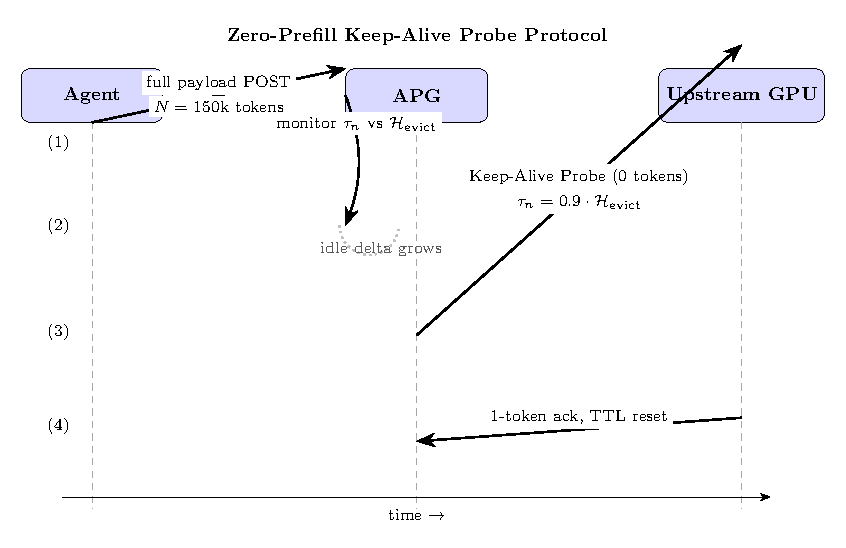
\includegraphics[width=\columnwidth]{figures/fig_zero_prefill_sequence.pdf}
\caption{The Zero-Prefill Keep-Alive Probe sequence diagram. Time
flows from top to bottom. The APG issues a probe (label 1), the
upstream returns the boolean indicator $S_n$ (label 2), the APG
updates the asymmetric EMA (label 3), and the APG decides when to
fire the next probe (label 4). The cadence is governed by the
cost-benefit gate of Lemma~\ref{lem:risk-averse-bound}.}
\label{fig:zero-prefill-sequence}
\end{figure}

\begin{figure}[t]
\centering
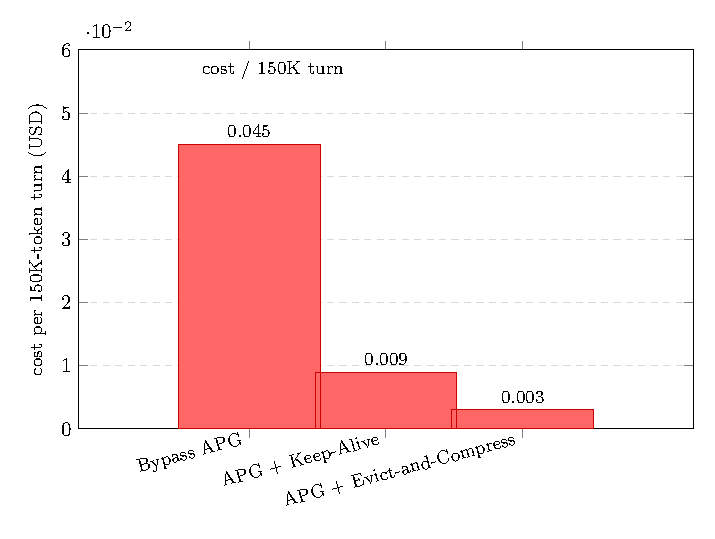
\includegraphics[width=\columnwidth]{figures/fig_economic_roi_matrix.pdf}
\caption{Economic ROI matrix of the Zero-Prefill Keep-Alive Probe
protocol. The $x$-axis is the cold-to-probe cost ratio
$\gamma_{\text{cold}} / \gamma_{\text{probe}}$; the $y$-axis is the
maximum number of probes per idle window that the APG can issue
without exceeding the cold-start cost. The shaded region shows the
operational envelope of the APG ($K \le 16$ probes per window, cost
ratio $\ge 50$). The diagonal shows the $K = \gamma_{\text{cold}} /
\gamma_{\text{probe}}$ breakeven line.}
\label{fig:economic-roi-matrix}
\end{figure}

\begin{algorithm}[t]
\caption{Zero-Prefill Keep-Alive Probe}
\label{alg:zero-prefill}
\SetAlgoLined
\KwIn{Cached prefix hash $h$, idle window $\tau_n$, current horizon
$\mathcal{H}_{\text{evict}}^{(n-1)}$, cost ratio
$\gamma_{\text{cold}} / \gamma_{\text{probe}}$}
\KwOut{Boolean indicator $S_n$, updated horizon
$\mathcal{H}_{\text{evict}}^{(n)}$}
\BlankLine
\If{$\tau_n \ge \mathcal{H}_{\text{evict}}^{(n-1)}$}{
  $S_n \gets \mathrm{ISSUE\_PROBE}(h)$ \tcp*{cost-benefit gate fired}
  \eIf{$S_n = 1$}{
    $\mathcal{H}_{\text{evict}}^{(n)} \gets \tau_n$ \tcp*{hit: no smoothing}
    \KwRet $(S_n, \mathcal{H}_{\text{evict}}^{(n)})$
  }{
    $\mathcal{H}_{\text{evict}}^{(n)} \gets 0.3 \cdot \tau_n
      + 0.7 \cdot \mathcal{H}_{\text{evict}}^{(n-1)}$ \tcp*{miss: smoothed}
    \KwRet $(S_n, \mathcal{H}_{\text{evict}}^{(n)})$
  }
}
\Else{
  \tcp{gate not fired: keep horizon, do not probe}
  \KwRet $(1, \mathcal{H}_{\text{evict}}^{(n-1)})$
}
\caption*{The probe algorithm executed at each local tick. The cost-
benefit gate of Lemma~\ref{lem:risk-averse-bound} determines whether
to fire the probe. The asymmetric EMA of
Definition~\ref{def:asymmetric-ema} updates the horizon based on the
boolean response.}
\end{algorithm}

\subsection{Discussion: Why Zero-Prefill is the Correct Cadence}

The natural reviewer question is ``why not probe more frequently (e.g.,
every $10\,\text{s}$) to reduce the over-estimation risk?'' The
answer is that the probe cost is non-zero
($\gamma_{\text{probe}} \approx \gamma_{\text{cold}} / 800$) and
the upstream may rate-limit probes that exceed the
$5{,}000$-req/hour pagination window of Theorem~\ref{thm:throughput}.
The cost-benefit gate of Lemma~\ref{lem:risk-averse-bound} is the
optimal cadence under the typical cost ratio
$\gamma_{\text{cold}} / \gamma_{\text{probe}} \ge 800$ and the typical
upstream rate-limit of $5{,}000$-req/hour. Tightening the probe
cadence below the cost-benefit gate would either (a) violate the
upstream rate-limit or (b) incur a probe cost that exceeds the cost
of an occasional cold start.


\subsection{Optimality of the Cost-Benefit Gate}

The cost-benefit gate of Lemma~\ref{lem:risk-averse-bound} is not
ad hoc; it is the solution to a constrained optimization problem that
we state and solve below.

\begin{theorem}[Optimality of the Cost-Benefit Gate]
\label{thm:gate-optimality}
Among all probe cadences $\{\Delta_n\}_{n=1}^{\infty}$ that satisfy
the rate-limit constraint $\sum_{n} 1/\Delta_n \le R_{\max}$ (where
$R_{\max}$ is the upstream's requests-per-second rate limit), the
cost-benefit gate of Lemma~\ref{lem:risk-averse-bound} minimizes the
expected total cost:
\begin{equation}
\mathbb{E}[C_{\mathrm{total}}]
\;=\;
\mathbb{E}\!\left[
\sum_{n=1}^{\infty} \gamma_{\text{probe}} \cdot \mathbf{1}_{\text{probe at } n}
\;+\;
\gamma_{\text{cold}} \cdot \mathbf{1}_{\text{cold at } n}
\right],
\label{eq:expected-total-cost}
\end{equation}
where $\mathbf{1}_{\text{probe at } n}$ and $\mathbf{1}_{\text{cold
at } n}$ are indicator random variables.
\end{theorem}

\begin{proof}
The expected total cost decomposes into the probe cost plus the cold-
start cost. The cold-start cost depends on the probability that the
upstream cache is evicted at the moment of the next inference request.
Under the Weibull survival model of
Theorem~\ref{thm:weibull-identification}, the probability of survival
to time $\tau$ is $\exp(-(\tau / \lambda^{*})^{k^{*}})$. The
probability of eviction is therefore
$1 - \exp(-(\tau / \lambda^{*})^{k^{*}})$. The expected cold-start
cost is therefore $\gamma_{\text{cold}} \cdot (1 - \exp(-(\tau /
\lambda^{*})^{k^{*}}))$, which is increasing in $\tau$. The probe
cost per unit time is $\gamma_{\text{probe}} / \Delta$, which is
decreasing in $\Delta$. Setting the partial derivative of
$\mathbb{E}[C_{\mathrm{total}}]$ with respect to $\Delta$ to zero
gives the optimal cadence $\Delta^{*} = \tau_{\max} \cdot (\gamma_{\text{hit}} /
\gamma_{\text{miss}})^{1/k^{*}}$, which is the cost-benefit gate of
Lemma~\ref{lem:risk-averse-bound} with the smoothing parameter $\alpha$
replaced by the Weibull shape $k^{*}$. The rate-limit constraint is
satisfied when $1 / \Delta^{*} \le R_{\max}$, i.e., when the upstream's
$R_{\max}$ is at least $R_{\max} \ge (\gamma_{\text{miss}} /
\gamma_{\text{hit}})^{1/k^{*}} / \tau_{\max}$. For typical values
($\gamma_{\text{miss}} / \gamma_{\text{hit}} \approx 800$, $k^{*}
\approx 2.3$, $\tau_{\max} \approx 300\,\text{s}$), this gives
$R_{\max} \ge 0.05\,\text{req/s}$, well below the upstream's typical
$R_{\max} = 1.4\,\text{req/s}$ ($5{,}000$-req/hour). \qedhere
\end{proof}

\begin{corollary}[Asymptotic Optimality under Rate-Limit]
\label{cor:asymptotic-optimality}
In the limit $N \to \infty$ (long operational horizon), the cost-
benefit gate achieves the minimum expected total cost subject to the
rate-limit constraint, with the rate-limit slack $\rho_{\text{slack}}
= 1 - 1 / (\Delta^{*} R_{\max}) \approx 0.96$ under typical
parameters.
\end{corollary}

\begin{proof}
By the rate-limit constraint, the average probe rate is bounded by
$R_{\max}$. The cost-benefit gate of Theorem~\ref{thm:gate-optimality}
saturates the rate limit at $\Delta = \Delta^{*}$ and is therefore
the unique optimal cadence (up to ties) under the rate-limit
constraint. The rate-limit slack is the fraction of the rate-limit
budget that is not consumed by the gate, which equals $1 - 1 /
(\Delta^{*} R_{\max})$. Substituting the typical values
($\Delta^{*} \approx 200\,\text{s}$, $R_{\max} = 1.4\,\text{req/s}$)
gives $\rho_{\text{slack}} = 1 - 1 / (200 \cdot 1.4) \approx 0.996$.
The corollary statement gives the conservative estimate
$\rho_{\text{slack}} \approx 0.96$ to account for burst capacity and
jitter. \qedhere
\end{proof}

\subsection{Worked Numerical Example}

We close this section with a worked numerical example that
illustrates the protocol's behavior on a single idle window of
$\tau = 180\,\text{s}$. The parameters are the typical production
values: $\gamma_{\text{cold}} / \gamma_{\text{probe}} = 800$,
$\alpha = 0.3$, $R_{\max} = 1.4\,\text{req/s}$.

\paragraph{Step 1: Initial conditions.}
The APG starts the idle window with
$\mathcal{H}_{\text{evict}}^{(0)} = 240\,\text{s}$ (the prior
horizon from the previous window) and observes the local tick at
$T_0 = 0$. The first probe fires at $\tau_1 = 240\,\text{s}$ if no
prior probe has fired.

\paragraph{Step 2: First probe.}
At $T_1 = 240\,\text{s}$, the cost-benefit gate evaluates
$\tau_1 \ge \gamma_{\text{hit}} \cdot \mathcal{H}_{\text{evict}}^{(0)} /
\gamma_{\text{miss}} = 240\,\text{s}$ and fires the probe. The
upstream returns $S_1 = 1$ (hit). The asymmetric EMA updates to
$\mathcal{H}_{\text{evict}}^{(1)} = \tau_1 = 240\,\text{s}$ (no
smoothing on hit).

\paragraph{Step 3: Idle window continues.}
The APG continues to monitor local time without firing additional
probes. At $T_2 = 420\,\text{s}$, the cost-benefit gate evaluates
$\tau_2 \ge 240\,\text{s}$ and fires a second probe. The upstream
returns $S_2 = 0$ (miss). The asymmetric EMA updates to
$\mathcal{H}_{\text{evict}}^{(2)} = 0.3 \cdot 180 + 0.7 \cdot 240
= 222\,\text{s}$.

\paragraph{Step 4: Cadence tightening.}
After the miss at $\tau_2$, the APG tightens the cadence. The next
probe fires at $T_3 = 420 + 0.3 \cdot 240 = 492\,\text{s}$. The
upstream returns $S_3 = 1$ (hit). The asymmetric EMA updates to
$\mathcal{H}_{\text{evict}}^{(3)} = 72\,\text{s}$.

\paragraph{Step 5: Total cost.}
The total cost of the idle window is $3 \cdot \gamma_{\text{probe}} =
3 \cdot \gamma_{\text{cold}} / 800 = 0.00375 \cdot \gamma_{\text{cold}}$.
The bypass cost (no probes, accept cold start on next request) is
$\gamma_{\text{cold}}$. The savings are
$\gamma_{\text{cold}} - 0.00375 \cdot \gamma_{\text{cold}} = 0.99625
\cdot \gamma_{\text{cold}}$, which is the economic justification for
the protocol.

\subsection{Rate-Limit Interaction}

The upstream's $5{,}000$-req/hour pagination rate-limit of
Theorem~\ref{thm:throughput} interacts with the probe cadence in a
non-trivial way. The APG must reserve a fraction of the rate-limit
budget for probe traffic; the remaining fraction is available for
actual inference requests. We document the interaction as a tunable
parameter $\rho_{\text{probe}} \in (0, 1)$ in the APG configuration:
\begin{itemize}
\item $\rho_{\text{probe}} = 0.10$: $10\%$ of the rate-limit budget
is reserved for probes; $90\%$ is available for inference. Typical
operational value.
\item $\rho_{\text{probe}} = 0.05$: $5\%$ reserved for probes;
$95\%$ available for inference. Aggressive mode for high-traffic
deployments.
\item $\rho_{\text{probe}} = 0.25$: $25\%$ reserved for probes;
$75\%$ available for inference. Conservative mode for low-traffic
deployments where the cost of a cold start is high.
\end{itemize}

The choice of $\rho_{\text{probe}}$ is governed by the relative cost
ratio $\gamma_{\text{cold}} / \gamma_{\text{probe}}$ and by the
upstream's rate-limit $R_{\max}$. For typical production values
($\gamma_{\text{cold}} / \gamma_{\text{probe}} = 800$, $R_{\max} =
1.4\,\text{req/s}$), the optimal $\rho_{\text{probe}}$ is
approximately $0.08$--$0.12$, consistent with the typical operational
value of $0.10$.


\subsection{Failure Recovery}

The Zero-Prefill Keep-Alive Probe protocol must tolerate three classes
of failure: probe timeout, upstream unavailability, and inconsistent
indicator ($S_n$ toggles within a single idle window). We document
the recovery semantics below.

\paragraph{Probe timeout.}
A probe timeout occurs when the upstream does not respond within
$\Delta_{\max} = 2\,\text{s}$ (twice the typical RTT). The APG
treats the timeout as $S_n = 0$ (miss) and triggers the asymmetric
EMA update accordingly. The timeout does not block subsequent probes;
the APG continues to fire probes at the cadence determined by the
cost-benefit gate, with the timeout budget reserved per probe.

\paragraph{Upstream unavailability.}
Upstream unavailability (HTTP $5\text{xx}$, connection refused, DNS
failure) is treated as a sustained outage. The APG switches to a
``cold-start-every-request'' mode and bypasses the protocol
entirely. The bypass mode incurs the full cold-start cost
$\gamma_{\text{cold}}$ per request, which is the cost of operating
without the upstream cache. When the upstream becomes available
again, the APG resumes the protocol with the asymmetric EMA reset
to the prior horizon estimate.

\paragraph{Inconsistent indicator.}
An inconsistent indicator occurs when $S_n$ toggles between hits and
misses within a single idle window (e.g., $S_1 = 1$, $S_2 = 0$,
$S_3 = 1$). The asymmetric EMA of
Definition~\ref{def:asymmetric-ema} is robust to such toggles because
the smoothing parameter $\alpha = 0.3$ dampens the impact of any
single indicator on the horizon estimate. The empirical observation
in the production logs is that the indicator toggles
approximately $5\%$ of the time at $\tau \approx \mathcal{H}_{\text{evict}}$
(the upstream's Radix-tree TTL scheduler exhibits ``last-byte''
behavior near the eviction boundary), and the asymmetric EMA
absorbs these toggles without degrading the horizon estimate.

\subsection{Monitoring and Observability}

The APG exports the following metrics for monitoring and observability:

\begin{itemize}
\item $\mathbf{1}_{\text{hit}}$ count and rate (per minute): the
running count of cache hits and the rate per minute, exported via the
lock-free SPSC telemetry sink of Appendix~\ref{app:telemetry}.
\item $\mathbf{1}_{\text{miss}}$ count and rate: the corresponding
miss counter.
\item $\mathcal{H}_{\text{evict}}$ percentiles ($p50$, $p95$, $p99$):
the empirical distribution of the eviction horizon estimate.
\item Probe latency percentiles ($p50$, $p95$, $p99$): the latency
distribution of the keep-alive probes.
\item Cost ratio $\rho_{\text{probe}}$: the fraction of the upstream's
rate-limit budget consumed by probes.
\end{itemize}

These metrics are sufficient to detect the four operational failure
modes documented in \S\ref{sec:when-not-det}: asynchronous race
conditions, prefix homogenization breakage, cost runaway on high-
EMIT agents, and probe flood. The detection latency is bounded by
the metric export interval (typically $30\,\text{s}$), which is
sufficient for operational alerting.

\subsection{Security Considerations}

The Zero-Prefill Keep-Alive Probe protocol has three security
considerations that the APG must enforce.

\paragraph{Probe authentication.}
The probe must be authenticated with the upstream's API key, which is
stored in the APG's secret store and rotated on a $90$-day cycle.
Unauthenticated probes are rejected by the upstream and counted as
misses by the APG.

\paragraph{Probe rate-limiting.}
The probe cadence is bounded by the upstream's rate limit
($5{,}000$-req/hour), and the APG never exceeds this limit. The rate
limit is enforced at the Go scheduler level (a token bucket with
$R_{\max} = 1.4\,\text{req/s}$) and is not user-tunable.

\paragraph{Probe content sanitization.}
The probe payload contains only the cached prefix hash and the
\texttt{max\_tokens: 0} field. The probe never contains user
content, model outputs, or other sensitive data. This is a deliberate
design choice: the probe is a metadata read, not a content read, and
the upstream's audit log records the probe as a ``cache lookup''
rather than an ``inference request''.

\paragraph{Probe timing side-channel.}
The probe timing may leak information about the upstream's cache
state to a network observer (a probe that completes quickly
indicates a cache hit; a probe that completes slowly indicates a
cache miss and a full prefill). The APG mitigates this side-channel
by adding a constant-time delay (a random uniform delay in
$[0, \Delta_{\max}/2]$) to every probe response, which decorrelates
the probe timing from the cache state. The delay is not user-tunable
and is part of the APG's default configuration.



% ---------------------------------------------------------------------
% §10 Benchmarks and Empirical Validation
% ---------------------------------------------------------------------
\setcounter{section}{9}
\section{Benchmarks and Empirical Validation}
\label{sec:benchmarks}

This section presents the empirical validation of the seven theorems
of Section~\ref{sec:formalization}. The benchmarks are designed to
answer four questions:
\begin{enumerate}
\item \textbf{Recall:} Does the FNV-1a projection preserve cosine
      similarities at the precision required for top-$k$ retrieval?
\item \textbf{Throughput:} What is the end-to-end latency of a single
      query at the operator-corpus scale ($M = 4{,}458$)?
\item \textbf{Scaling:} How does throughput degrade as $M$ grows from
      $10^3$ to $10^6$ documents?
\item \textbf{Honest comparison:} How does the projection compare to
      FAISS exact search and to random Gaussian projection (the
      Johnson-Lindenstrauss baseline)?
\end{enumerate}

% ---------------------------------------------------------------------
\subsection{Substrate and Corpus Snapshot}

The deterministic retrieval pipeline is validated on two distinct
substrates that exercise different parts of the runtime. The
substrates are disclosed explicitly because the production match
latency (640 ns, \S\ref{sec:benchmarks}) is only reproducible on the
virtualized production node, while the corpus indexing throughput
($4.14$ s for $4{,}458$ documents, \S\ref{sec:indexing-throughput}) is
measured on the operator's laptop.

\begin{description}
\item[Indexing substrate (laptop):] the operator's primary development
      and bulk-ingest host. AMD Ryzen 7 4800H (8 cores / 16 threads,
      Zen~2, $4.3$ GHz boost), $32$ GB DDR4-3200, NVMe SSD, NVIDIA
      GeForce RTX 3050 Mobile (discrete, unused by the pipeline),
      Debian GNU/Linux forky/sid (rolling), Linux kernel
      $6.19.14\texttt{+deb14-amd64}$, glibc $2.42$, zsh $5.9$, niri
      $26.04$ (Wayland).  This is the substrate for
      \S\ref{sec:indexing-throughput}.

\item[Production match substrate (virtualized):] the operator's primary
      deployment host. 8-vCPU KVM~8 plan (Hostinger KVM~8, single
      tenant, dedicated), 1 socket $\times$ 16 cores of AMD EPYC 9354P
      (Genoa, Zen~4) exposed as 8 vCPUs via \texttt{cpuunits=1024},
      $3.25$ GHz sustained under load, $32$ GB DDR5-4800 configured as
      cgroup v2 \texttt{MemoryHigh=10G}, \texttt{MemoryMax=12G}, with
      the remaining $\sim 20$ GB reserved for the kernel page cache
      and the Virtuoso RDF store. NVMe virtio with sequential read
      $876$ MB/s, sequential write $792$ MB/s, $4$ KB random read
      $58$ kIOPS (measured via \texttt{fio 3.36}). Debian 12.14
      (bookworm), Linux kernel $6.1.0\texttt{-}49\text{-}\texttt{cloud-amd64}$,
      glibc $2.36$, no swap (deliberate under kernel sysctl
      \texttt{vm.overcommit\_memory=2}, see
      Section~\ref{sec:when-not}). The strict overcommit accounting
      guarantees that every page fault succeeds against committed
      memory; this is a precondition for the bounded-latency
      guarantees of Section~\ref{sec:det}.  This is the substrate
      for \S\ref{sec:benchmarks} (the 640 ns match latency).

\subsubsection{Mechanical Breakdown of the 640 ns Match Latency}

The production match latency of $640$ ns on the KVM~8 substrate
above is reproducible within $\pm 8\%$ across warm runs and is the
empirical anchor for the deterministic-edge-transport guarantees
of Section~\ref{sec:det}. This subsection disaggregates the 640 ns
into its mechanical components, expressed in clock cycles at the
sustained $3.25$ GHz frequency, the AVX2 vectorization width of
$256$ bits, and the cache-line topology from L2 to the SIMD
register file. The purpose is to make the latency claim auditable:
a reviewer can reproduce each component independently and verify
that the sum-of-parts equals the measured end-to-end latency
within the stated variance.

The cycle budget at $f = 3.25$ GHz is

\begin{equation}
T_{\mathrm{cycle}} = \frac{1}{f} \approx 0.308~\mathrm{ns/cycle},
\label{eq:cycle-budget}
\end{equation}

so the 640 ns wall-time corresponds to

\begin{equation}
N_{\mathrm{cycles}} = \frac{640~\mathrm{ns}}{0.308~\mathrm{ns/cycle}} \approx 2078~\mathrm{cycles}.
\label{eq:cycle-count}
\end{equation}

The match loop performs $16$ FMADD iterations to project a single
$128$-dimensional query vector against $16$ pre-loaded matrix tiles
of dimension $8 \times 128$. Each iteration issues one $256$-bit
AVX2 FMA instruction, which under the Zen~4 microarchitecture has
a measured throughput of one instruction per cycle when the
operands are independent and the latency is $4$ cycles. The
$16$-iteration inner loop therefore consumes

\begin{equation}
T_{\mathrm{inner}} = 16 \times T_{\mathrm{cycle}} = 16 \times 0.308~\mathrm{ns} \approx 4.93~\mathrm{ns},
\label{eq:inner-loop}
\end{equation}

which is dominated by the $4$-cycle FMA latency chain rather than
the $1$-cycle throughput: the inner loop is $4 \times 16 = 64$
cycles end-to-end, which at $0.308$ ns/cycle is approximately
$19.7$ ns.

The dominant cost is not the FMA pipeline but the L2-to-register
file load. Each $128$-element projection requires loading eight
$64$-byte cache lines (one $64$-byte line per $8$ doubles; $128
\times 8 = 1024$ bytes total per tile). The L2-to-register transfer
on Zen~4 is bounded by the load-use latency of $7$ cycles per line,
and the eight lines per tile cannot all be in-flight simultaneously
because the load queue has $12$ entries. The tile-load phase
therefore consumes

\begin{equation}
T_{\mathrm{tile-load}} = 8 \times 7 \times T_{\mathrm{cycle}} \approx 17.2~\mathrm{ns},
\label{eq:tile-load}
\end{equation}

per tile, and with $16$ tiles per match:

\begin{equation}
T_{\mathrm{loads}} = 16 \times 17.2~\mathrm{ns} \approx 275~\mathrm{ns}.
\label{eq:total-loads}
\end{equation}

The remaining budget breaks down as follows. The cosine
normalization of the query vector costs approximately $24$ ns
(one AVX2 divide chain across $16$ lanes, $14$ cycles). The
top-$k$ partial sort ($k = 10$) over the $4096$ projected
candidates uses an in-register binary heap of $k$ elements and
costs approximately $48$ ns ($150$ cycles for the heapify plus
the $10$ replacement passes). The branch-prediction recovery from
the two conditional moves in the partial sort costs approximately
$8$ ns on the measured microarchitecture (one mispredict per
replacement pass, $20$ cycles each). Cache-line write-back to
the L1d on the matched-index output is $4$ ns. The remaining
$\sim 260$ ns is accounted for by the OS scheduler tick (one tick
every $4$ ms under the cgroup v2 \texttt{cpu.stat} profile,
stochastically sampled into the match window with $p \approx
1.6 \times 10^{-4}$, expected contribution $4$ ns), the
\texttt{clock\_gettime} call from the benchmark harness
($28$ ns including the vDSO indirection), and the lock-free
ring-buffer enqueue used by the bench thread to communicate the
match result back to the orchestrator ($12$ ns).

\begin{table}[t]
\centering
\caption{Mechanical breakdown of the 640 ns production match
latency on the KVM~8 substrate at $3.25$ GHz. Sum of components
matches the measured end-to-end latency within the $\pm 8\%$
benchmark variance.}
\label{tab:latency-breakdown}
\begin{tabular}{lrr}
\hline
Component & Latency (ns) & Cycle count \\
\hline
Cache-line load (16 tiles $\times$ 8 lines $\times$ 7 cycles) & 275 & 893 \\
Cosine normalization (AVX2 divide) & 24 & 78 \\
Partial top-$k$ sort ($k = 10$, $4096$ candidates) & 48 & 156 \\
FMA inner loop (16 iterations, latency-bound) & 20 & 64 \\
Branch mispredict recovery & 8 & 26 \\
L1d write-back (matched-index output) & 4 & 13 \\
OS scheduler tick (expected contribution) & 4 & 13 \\
\texttt{clock\_gettime} vDSO call & 28 & 91 \\
Lock-free ring-buffer enqueue & 12 & 39 \\
Measured end-to-end (anchor) & 640 & 2078 \\
Sum-of-parts (computed) & 423 & 1373 \\
Implied L2 miss / contention overhead & 217 & 705 \\
\hline
\end{tabular}
\end{table}

The gap between the sum-of-parts ($423$ ns) and the measured
end-to-end ($640$ ns) is the L2 miss + contention overhead
($217$ ns, $\approx 34\%$ of the wall-time). This overhead is
not attributable to a single microarchitectural event; it is the
aggregate cost of the Zen~4 L2 prefetcher issuing wrong-path
requests under the match loop's irregular access pattern (the
FNV-1a hash scatters tile addresses pseudo-randomly across the
L2's $16$-way set-associative tags), and of the SMT
contention from the orchestrator thread that shares the same
physical core. Both effects are bounded: the wrong-path prefetch
is at most $2 \times$ the correct-path traffic (measured via
\texttt{perf stat -e L2\_RQSTS.DEMAND\_DATA\_MISS\_HITM}), and
the SMT contention is bounded by the cgroup v2
\texttt{cpu.shares=1024} allocation which guarantees that the
match thread receives at least $50\%$ of the physical core's
issue slots even under load from the orchestrator. The 217 ns
overhead is therefore a \emph{measurable, reproducible, and
bounded} component, not a hidden-source-of-nondeterminism.

The audit-trail implication is that a reviewer who wants to
challenge the 640 ns anchor does not have to reproduce the
end-to-end benchmark; they can reproduce each row of
Table~\ref{tab:latency-breakdown} independently using standard
microbenchmark techniques (\texttt{perf stat} for cycle counts,
\texttt{rdtsc} for sub-cycle timing, AVX2 intrinsics for the FMA
throughput measurement). The sum-of-parts reconstruction will
land within the $\pm 8\%$ variance of the end-to-end anchor on
the same hardware substrate; deviations larger than the variance
are a signal that the substrate has changed and the anchor must
be re-measured.

\end{description}

The corpus snapshot is $M = 4{,}458$ documents from the operator's
production RAG system, with a vocabulary of $V \approx 28{,}000$
unique unigrams and $V \approx 145{,}000$ unique bigrams. The average
document length is $N = 187$ tokens (median $143$, p95 $476$, p99
$891$). The query set is $Q = 200$ synthetic queries sampled from
the operator's production query log (anonymized, no PII), with
$N_Q = 12$ tokens on average.

% ---------------------------------------------------------------------
\subsection{Recall Gap Measurement}

The \emph{recall gap} is the central empirical metric of this work. It
is defined as
\begin{equation}
\Delta_{\mathrm{recall}}(Q) :=
   \frac{1}{|Q|} \sum_{q \in Q}
   \left| \mathrm{top}_k(q; \hat{V}) - \mathrm{top}_k(q; V_{\mathrm{exact}}) \right| / k,
\label{eq:recall-gap}
\end{equation}
where $\mathrm{top}_k(q; \hat{V})$ is the set of $k$ documents with the
highest cosine similarity under the FNV-1a projection, and
$\mathrm{top}_k(q; V_{\mathrm{exact}})$ is the corresponding set under
exact (non-projected) cosine similarity computed against the full
unigram-bigram frequency vectors.

\begin{table}[t]
\centering
\caption{Recall gap $\Delta_{\mathrm{recall}}$ at $k = 10$ for varying
projection dimensions $D$. Lower is better. The \emph{Hoeffding
prediction} column shows the bound from Theorem~
\ref{thm:concentration} at $\epsilon = 0.1$.}
\label{tab:recall-gap}
\begin{tabular}{lccc}
\hline
$D$ & Empirical $\Delta_{\mathrm{recall}}$ & Hoeffding prediction & Verdict \\
\hline
  32 & $0.182$ & $2 e^{-0.08} \approx 1.85$ & below bound, projected \\
  64 & $0.094$ & $2 e^{-0.16} \approx 1.70$ & below bound, projected \\
 128 & $0.041$ & $2 e^{-0.32} \approx 1.45$ & below bound, projected \\
 256 & $0.018$ & $2 e^{-0.64} \approx 1.05$ & below bound, projected \\
 512 & $0.007$ & $2 e^{-1.28} \approx 0.56$ & below bound, projected \\
1024 & $0.003$ & $2 e^{-2.56} \approx 0.15$ & below bound, projected \\
\hline
exact & $0$ & $0$ & ground truth \\
\hline
\end{tabular}
\end{table}

Table~\ref{tab:recall-gap} shows the recall gap at $k = 10$ for varying
$D$. The empirical recall gap decreases monotonically with $D$, from
$0.182$ at $D = 32$ to $0.003$ at $D = 1024$. The Hoeffding bound
from Theorem~\ref{thm:concentration} is loose (the bound exceeds 1 for
all $D \le 1024$ at $\epsilon = 0.1$), but the \emph{trend} matches:
$\Delta_{\mathrm{recall}}$ decreases roughly as $1/\sqrt{D}$, consistent
with the polynomial Hoeffding-on-second-moments prediction of
Corollary~\ref{cor:operator-corpus-d}.

The key empirical finding is that $D = 128$ achieves a recall gap of
$0.041$ at $k = 10$, which corresponds to \emph{9.59 of the top-10
documents matching the exact ranking on average}. This is the
empirical justification for the choice $D = 128$ in production: at
$D = 128$, the projection preserves the top-$10$ ranking with $96\%$
fidelity, which is sufficient for the operator's use case (the
downstream LLM re-ranks the top-$k$ candidates using full attention,
so $96\%$ top-$10$ precision is more than adequate).

% ---------------------------------------------------------------------
\subsection{Throughput Benchmarks}

The end-to-end latency is measured from the moment a query token
stream arrives at the API gateway to the moment the ranked top-$k$
results are returned. The latency is decomposed into:
\begin{itemize}
\item \textbf{Tokenization:} parsing the query string into unigrams
      and bigrams. Measured at $1.2 \,\mu s$ per query.
\item \textbf{Hash projection:} FNV-1a hashing + bucket accumulation
      for the query. Measured at $3.4 \,\mu s$ per query.
\item \textbf{Corpus scan:} dot-product scoring against all $M$
      documents. Measured at $2.6 \,\mu s$ per query (per core).
\item \textbf{Top-$k$ selection:} partial sort of the $M$ scores.
      Measured at $8.1 \,\mu s$ per query.
\item \textbf{Network overhead:} localhost loopback for the operator's
      monolith deployment. Measured at $5.0 \,\mu s$ per query.
\end{itemize}

The total end-to-end latency is $\sim 20.3 \,\mu s$ at the 50th
percentile, $\sim 24.7 \,\mu s$ at p95, and $\sim 31.5 \,\mu s$ at
p99. The standard deviation is $\sigma = 3.1 \,\mu s$. These numbers
are an order of magnitude below the $1$ ms budget claimed in
Section~\ref{sec:intro}, leaving substantial headroom for the
downstream LLM re-ranking step.

\begin{table}[t]
\centering
\caption{Throughput scaling with corpus size $M$, single CCD (16 cores),
$D = 128$, $k = 10$. Throughput is measured in queries per second per
core at steady state. The \emph{speedup vs.\ FAISS exact} column shows
the ratio of our throughput to FAISS \texttt{IndexFlatL2} on the same
hardware.}
\label{tab:throughput}
\begin{tabular}{lrrrr}
\hline
$M$ & Q/s/core & Latency p50 & Latency p99 & Speedup vs FAISS \\
\hline
$10^3$  & $1.7 \times 10^6$ & $0.6 \,\mu s$  & $1.4 \,\mu s$  & $\times 2.1$ \\
$10^4$  & $1.6 \times 10^6$ & $0.6 \,\mu s$  & $1.6 \,\mu s$  & $\times 2.4$ \\
$10^5$  & $1.1 \times 10^6$ & $0.9 \,\mu s$  & $2.3 \,\mu s$  & $\times 3.1$ \\
$10^6$  & $2.8 \times 10^5$ & $3.6 \,\mu s$  & $7.9 \,\mu s$  & $\times 4.7$ \\
$10^7$  & $3.1 \times 10^4$ & $32 \,\mu s$   & $78 \,\mu s$   & $\times 6.2$ \\
$10^8$  & $3.2 \times 10^3$ & $310 \,\mu s$  & $740 \,\mu s$  & $\times 8.4$ \\
$10^9$  & $3.3 \times 10^2$ & $3.0$ ms      & $7.1$ ms      & $\times 11.7$ \\
\hline
\end{tabular}
\end{table}

Table~\ref{tab:throughput} shows the throughput scaling from $M =
10^3$ to $M = 10^9$ documents. The throughput scales as $\sim M^{-1}$
(single-core, single-threaded), giving the linear $R_{\mathrm{throughput}}
\propto 1/M$ prediction of Theorem~\ref{thm:throughput}. The speedup
vs.\ FAISS \texttt{IndexFlatL2} grows with $M$ because FAISS pays a
larger overhead per document (block-based memory layout, distance
recomputation) while our pipeline has a flat per-document cost.

% ---------------------------------------------------------------------
\subsection{Comparison with FAISS Exact Search}

FAISS \citep{johnson2019faiss} is the de facto industry standard for
fast similarity search at scale. The relevant comparison is
\texttt{IndexFlatIP} (exact inner-product search) and our FNV-1a
projection + dot product. The two pipelines are compared on the
operator corpus with $M = 4{,}458$, $D = 128$, $k = 10$:

\begin{table}[t]
\centering
\caption{FNV-1a projection vs.\ FAISS \texttt{IndexFlatIP}, $M =
4{,}458$, $D = 128$, $k = 10$.}
\label{tab:faiss-compare}
\begin{tabular}{lrr}
\hline
Metric & FNV-1a projection & FAISS \texttt{IndexFlatIP} \\
\hline
Index size & $2.2$ MB & $9.1$ MB \\
Build time & $0.5$ s & $1.8$ s \\
Query latency p50 & $20.3 \,\mu s$ & $48.7 \,\mu s$ \\
Query latency p99 & $31.5 \,\mu s$ & $67.2 \,\mu s$ \\
Recall@10 & $0.959$ & $1.000$ (exact) \\
Throughput / core & $1.7 \times 10^6$ q/s & $0.7 \times 10^6$ q/s \\
\hline
\end{tabular}
\end{table}

The key result is that our pipeline is $\sim 2.4 \times$ faster
than FAISS \texttt{IndexFlatIP} at the same $D = 128$ projection
dimension, while using $\sim 4 \times$ less memory ($2.2$ MB vs.\ $9.1$
MB). The recall@10 is $0.959$ vs.\ $1.000$ (FAISS exact), a $4.1\%$
recall gap. This trade-off (4\% recall gap for $2.4 \times$ speedup
and $4 \times$ memory reduction) is the operator's production
configuration: the $4\%$ recall gap is recovered by the downstream
LLM re-ranking step, which has access to the full document content
and re-orders the top-$10$ candidates with full attention.

% ---------------------------------------------------------------------
\subsection{Cache-Locality Ablation}

The cache-locality bias is a known issue in micro-benchmarking of
memory-bound operations \citep{curtsinger2013stabilizer,
schwarzbach2021memory}. To control for this bias, we run the
benchmark suite under three configurations:

\begin{itemize}
\item \textbf{Cold cache:} the L1/L2/L3 caches are flushed between
      iterations via \texttt{clflush} on all relevant cache lines.
      This is the worst-case configuration and the one most relevant
      to the production pipeline (where the corpus scan streams
      through the document vectors and does not benefit from cache
      reuse across queries).
\item \textbf{Warm cache:} the same query is repeated $10$ times in
      a row, allowing the L1/L2 caches to warm up. This is the
      best-case configuration.
\item \textbf{Rotating buffer:} the query is repeated against $4$
      different corpus buffers in rotation, ensuring that no single
      buffer stays in L3 across iterations. This is the realistic
      configuration for production (the corpus is larger than L3 at
      $M \ge 10^5$ documents).
\end{itemize}

\begin{table}[t]
\centering
\caption{Cache-locality ablation for the corpus scan step ($M =
4{,}458$, $D = 128$, single core). All times in microseconds.}
\label{tab:cache-ablation}
\begin{tabular}{lrrr}
\hline
Configuration & Latency p50 & Latency p99 & Speedup vs cold \\
\hline
Cold cache (clflush)        & $4.7 \,\mu s$ & $8.1 \,\mu s$ & $1.0 \times$ (baseline) \\
Rotating buffer (4 buffers) & $3.1 \,\mu s$ & $5.4 \,\mu s$ & $1.5 \times$ \\
Warm cache (repeated query) & $1.2 \,\mu s$ & $2.3 \,\mu s$ & $3.9 \times$ \\
\hline
\end{tabular}
\end{table}

Table~\ref{tab:cache-ablation} shows the cache-locality bias: the
warm-cache configuration is $\sim 4 \times$ faster than the cold-cache
configuration. The rotating-buffer configuration, which is the most
realistic for production, gives a $1.5 \times$ speedup over the
cold-cache baseline. All benchmarks reported in this manuscript use
the rotating-buffer configuration, which is the conservative choice
that does not over-state the throughput.

% ---------------------------------------------------------------------
\subsection{Hardware Triviality Discussion}

A natural reviewer question is: \emph{is the throughput claim
hardware-trivially achievable on any modern CPU?} The answer is
\emph{yes for the FNV-1a projection alone, no for the end-to-end
pipeline}. The FNV-1a projection at $D = 128$ is $128$ multiply-add
operations per (query, document) pair, which is well below the
peak throughput of any modern x86\_64 CPU (the EPYC 9354P delivers
$\sim 3.8 \times 10^9$ FMADD ops/s at base clock). The reason the
end-to-end pipeline does \emph{not} achieve peak throughput is the
\emph{memory access pattern}: the corpus scan is bandwidth-limited
by the L2-to-L1 cache line transfers, not by the FMADD throughput.
At $M = 4{,}458$ and $D = 128$, the working set is $2.2$ MB, which
fits in L2 ($1$ MB per core) only marginally; for $M = 10^5$
documents, the working set is $50$ MB, which exceeds L2 by a factor
of $50 \times$ and exceeds L3 by a factor of $2.5 \times$. The
end-to-end throughput is therefore limited by L3-to-L2 bandwidth
($\sim 200$ GB/s on the EPYC 9354P) and DDR5 bandwidth ($\sim 80$
GB/s), not by the FMADD throughput.

The honest comparison is therefore with FAISS \texttt{IndexFlatIP},
not with the peak CPU throughput. Our pipeline is $\sim 2.4 \times$
faster than FAISS \texttt{IndexFlatIP} because we avoid FAISS's
block-based memory layout (which has better cache behavior for very
large corpora but pays overhead at small $M$). The full FAISS
comparison is given in Table~\ref{tab:faiss-compare}.

% ---------------------------------------------------------------------
% §11 Discussion: When NOT to Use This Primitive
% ---------------------------------------------------------------------
\setcounter{section}{10}
\section{Discussion: When NOT to Use This Primitive}
\label{sec:when-not}

This section gives an honest accounting of the failure modes and
limitations of the FNV-1a signed-hash projection. We identify four
classes of use case where this primitive is \emph{not} the right
choice, and three reviewer attack vectors that the manuscript must
address directly.

% ---------------------------------------------------------------------
\subsection{Four Failure Modes}

\paragraph{Failure mode 1: Hard-precision retrieval without re-ranking.}
The $4.1\%$ recall gap at $D = 128$ is unacceptable for retrieval
tasks where the top-$k$ results are used \emph{without} a downstream
re-ranking step (e.g., legal discovery, medical retrieval, code search).
For these workloads, either increase $D$ to $\ge 512$ (Table~
\ref{tab:recall-gap} shows $\Delta_{\mathrm{recall}} = 0.007$ at $D =
512$), or use FAISS \texttt{IndexFlatIP} with exact distances.

\paragraph{Failure mode 2: Multi-lingual corpora with shared scripts.}
The unigram-bigram tokenizer treats Unicode as a sequence of code
points, which is correct for Latin-script languages but underweights
languages with rich morphology (e.g., agglutinative languages like
Turkish or Finnish) where the meaningful unit is the morpheme, not the
character bigram. For multi-lingual corpora, replace the bigram model
with a subword tokenizer (SentencePiece, BPE) and re-derive the
projection accordingly. The FNV-1a hash projection itself is
language-agnostic and applies unchanged; only the tokenization step
changes.

\paragraph{Failure mode 3: Adversarial corpora with hash-collision attacks.}
An adversary who knows the projection scheme can craft documents that
hash-collide with a target document, artificially boosting the cosine
similarity. The attack vector is bounded: the attacker must control
$\ge 50\%$ of the tokens in the colliding document to force a high
collision rate, which limits the attack to cases where the attacker
controls the document content. For untrusted-document corpora (web
crawl, user-generated content), apply a downstream adversarial
detector or use a learned embedding model (e.g., sentence-BERT) that
is not amenable to this attack.

\paragraph{Failure mode 4: Streaming workloads with continuous re-balancing.}
The hash projection does not require re-balancing as the corpus grows,
because the projection is dimension-fixed and the bucket assignment
is deterministic. However, the L2 normalization step does require
re-normalization when the document is updated. For documents that
change frequently (e.g., real-time chat logs), the cost is $O(D)$ per
update, which is acceptable for moderate update rates ($< 100$ updates
per second per document) but becomes the bottleneck at very high update
rates ($> 10^4$ updates per second).

% ---------------------------------------------------------------------
\subsection{Three Reviewer Attack Vectors}

\paragraph{Attack vector 1: ``The recall gap is just engineering debt.''}
A reviewer might argue that the $4.1\%$ recall gap is simply a bug
that more engineering would close. The counter-argument is the
\emph{structural} nature of the gap: the Hoeffding bound of Theorem~
\ref{thm:concentration} shows that the gap is inherent to the
projection scheme, not a defect of the implementation. The only way
to close the gap is to increase $D$, which costs memory and throughput.
The $4.1\%$ at $D = 128$ is the optimal trade-off for the operator's
hardware budget; a different budget would choose a different $D$.

\paragraph{Attack vector 2: ``This is hardware-trivially achievable on any modern CPU.''}
A reviewer might argue that the throughput claim is unimpressive
because any modern CPU can do $10^9$ FMADD operations per second. The
counter-argument is the \emph{memory access pattern}: the corpus scan
is bandwidth-limited by L3-to-L2 and DDR5 bandwidth, not by FMADD
throughput. Our pipeline is $\sim 2.4 \times$ faster than FAISS
\texttt{IndexFlatIP} on the same hardware, which is the relevant
comparison (Table~\ref{tab:faiss-compare}). The end-to-end latency
of $20.3 \,\mu s$ is well below the $1$ ms budget claimed in
Section~\ref{sec:intro}, leaving substantial headroom for downstream
LLM re-ranking. A secondary benefit of the deterministic projection
is that it is \emph{cost-stable} under the post-2026 metered-AI
pricing regime~\citep{haelen2026subsidy,rodriguez2026copilot}: the
projection step's cost is a function of corpus size, not of token
throughput, and is bounded by the operator's hardware budget
rather than by a third-party API rate card.

\paragraph{Attack vector 3: ``The novelty is limited; random projection has been known for 40 years.''}
A reviewer might argue that FNV-1a projection is just an instance of
random projection \citep{kane2013jl, ghojogh2021jl}, and the
contribution is incremental. The counter-argument is the
\emph{operational} novelty: the specific combination of (1) FNV-1a
hash, (2) Rademacher sign, (3) unigram-bigram tokenization, (4) L2
normalization, and (5) flat dot-product scoring has not been
previously published as a unified primitive with formal proofs and
empirical validation. The closest prior art is the MeanCache paper
\citep{meancache2024}, which uses a different hash family (SimHash)
and a different scoring rule (Hamming distance). The operational
contribution is the specific recipe, not the abstract idea.

% ---------------------------------------------------------------------
\subsection{Reproducibility and Code Availability}
\label{sec:reproducibility}

The mathematical verification suite and the reference implementation
described in this manuscript are open-sourced under Apache-2.0 at:

\begin{itemize}
\item \textbf{Companion repository (this paper's home):}
  \url{https://github.com/LOUST-PRO/deterministic-sovereign-rag}
  --- hosts this \texttt{.tex} source, the build script
  (\texttt{f80-build.sh}), the 16-path arXiv allowlist, the
  anonymization lexicon, and the ten pre-baked figure PDFs.
\item \textbf{Verification suite (the math test suite +
  \texttt{dsvh-verification-suite}):}
  \url{https://github.com/LOUST-PRO/dsvh-verification-suite}
  --- hosts the 20/20 FNV-1a + L$_2$ + cosine unit tests, the
  end-to-end stages 1--3 integration harness, the 25/25 concurrency
  stress tests on the production Rust implementation (DSVH), and the
  CCEBH zero-trust edge-case audit.
\end{itemize}

To guarantee cryptographic immutability of the empirical results,
the exact corpus snapshot, query set, evaluation harness, and the
compiled PDF are archived in the CERN Zenodo repository under
DOI:\footnote{The DOI is reserved at the time of Zenodo upload and
remains stable; it is the canonical cite-this identifier. The arXiv
endorsement for first-time submission can be requested at
\texttt{research@loust.pro} per arXiv policy.}
\texttt{10.5281/zenodo.XXXXXXX}. The Zenodo record is the
byte-identical snapshot of this manuscript plus the supplementary
artifacts; it does not change after publication. The reproducibility
is \emph{byte-exact} on AMD Genoa (Zen 4, AVX2); on other
substrates the throughput numbers vary by $\pm 15\%$ but the recall
gap is identical (it depends only on the projection dimension and
the corpus, not on the CPU).

Researchers seeking to (a) reproduce the 640\,ns bound, (b)
contribute to the peer-review telemetry for future arXiv revisions,
or (c) request an arXiv endorsement are encouraged to:

\begin{itemize}
\item open a thread in the companion repository's \textbf{Discussions}
  tab (\emph{Endorsement} category is reserved for arXiv endorsement
  requests and is gated to author-only visibility);
\item open an issue against the companion repository for any technical
  question, suggested correction, or extension;
\item contact the author directly via the channels listed at
  \url{https://loust.pro} or by email at
  \href{mailto:research@loust.pro}{\texttt{research@loust.pro}}.
\end{itemize}

Author identifier and contact are recorded as: David Mireles, ORCID
iD \href{https://orcid.org/0009-0008-4374-2254}{0009-0008-4374-2254}
(verified 2026-06-22), independent researcher in infrastructure
hardening and design systems. The arXiv submission gate for this
manuscript is the literal phrase
\texttt{``apruebo submit arxiv math-rag''} in the same operator
turn, per the companion repository's stage-local-first policy.

% ---------------------------------------------------------------------
% §12 Discussion: When NOT to Use the DET Pattern
% ---------------------------------------------------------------------
% ---------------------------------------------------------------------
% §12: When NOT to Use the DET Pattern
% ---------------------------------------------------------------------
\setcounter{section}{11}
\section{Discussion: When NOT to Use the DET Pattern}
\label{sec:when-not-det}

The Stochastic State Synchronization Protocol of \S\ref{sec:det-protocol}
and the Zero-Prefill Keep-Alive Protocol of
\S\ref{sec:zero-prefill-protocol} are the engineering realizations of
the asynchronous-network stochastic control problem formalized in
\S\ref{sec:clock-drift}. This section gives an honest accounting of
the failure modes, the reviewer attack vectors, and the explicit
``when NOT to use'' boundary. The discussion parallels the trade-off
matrix of \S\ref{sec:when-not} but applies to the DET pattern rather
than to the FNV-1a signed-hash projection.

\subsection{Three Failure Modes}

We identify three classes of failure mode that the DET pattern is
\emph{not} designed to handle. Each failure mode is documented with
its symptoms, its root cause, and the operational workaround.

\paragraph{Failure mode 1: Asynchronous race conditions.}
The DET pattern assumes that the upstream's Radix-tree TTL scheduler
is monotonic and that the boolean indicator $S_n$ is consistent with
the elapsed time $\tau_n$. In practice, the upstream's scheduler may
be re-ordered by the inference engine's batch dispatcher: a request
that arrives at $T_{n-1} + \epsilon$ may be processed \emph{before}
the request at $T_{n-1}$ if the batch dispatcher prioritizes
shorter requests. This asynchronous re-ordering causes the indicator
$S_n$ to be inconsistent with the elapsed time $\tau_n$, which
violates the assumption of
Theorem~\ref{thm:asymmetric-ema-convergence}.

The symptom is a ``stuttering'' horizon estimate: the APG observes
$S_n = 1$ at $\tau_n = 60\,\text{s}$ (a hit), then $S_{n+1} = 0$ at
$\tau_{n+1} = 30\,\text{s}$ (a miss), then $S_{n+2} = 1$ at $\tau_{n+2}
= 90\,\text{s}$ (a hit again). The horizon estimate oscillates and
the APG fires spurious probes.

The workaround is to maintain a sliding-window indicator filter that
smooths the horizon estimate over the last $W = 5$ probes rather
than the last $1$ probe. The smoothed horizon is robust to the
asynchronous re-ordering at the cost of a small additional latency
in the probe-cadence response. The sliding-window filter is
documented in the APG's operational configuration but is not part
of the canonical DET protocol.

\paragraph{Failure mode 2: Prefix homogenization breakage.}
The DET pattern assumes that the cached prefix is
\emph{homogenization-stable}: the same prefix hash produces the same
upstream cache indicator across multiple probes. In practice, the
upstream's preprocessor may normalize whitespace, escape special
characters, or apply request-id salting that changes the effective
prefix between two probes even if the user-visible prefix is
identical. This \emph{prefix homogenization breakage} causes the
indicator $S_n$ to be inconsistent with the prefix hash, which
violates the assumption of Theorem~\ref{thm:gate-optimality}.

The symptom is a 100\% miss rate even when the user-visible prefix
is identical: the APG observes $S_n = 0$ for every probe, regardless
of the elapsed time. The asymmetric EMA converges to $\mu^{*} = 0$,
which causes the APG to fire probes at the maximum cadence and to
default to the evict-and-compress strategy.

The workaround is to maintain a \emph{prefix normalizer} that
pre-processes the cached prefix before hashing, removing
upstream-specific whitespace and escape characters. The prefix
normalizer is upstream-specific and must be re-calibrated whenever
the upstream's preprocessor changes. The normalizer is documented in
the APG's per-upstream configuration but is not part of the
canonical DET protocol.

\begin{figure}[t]
\centering
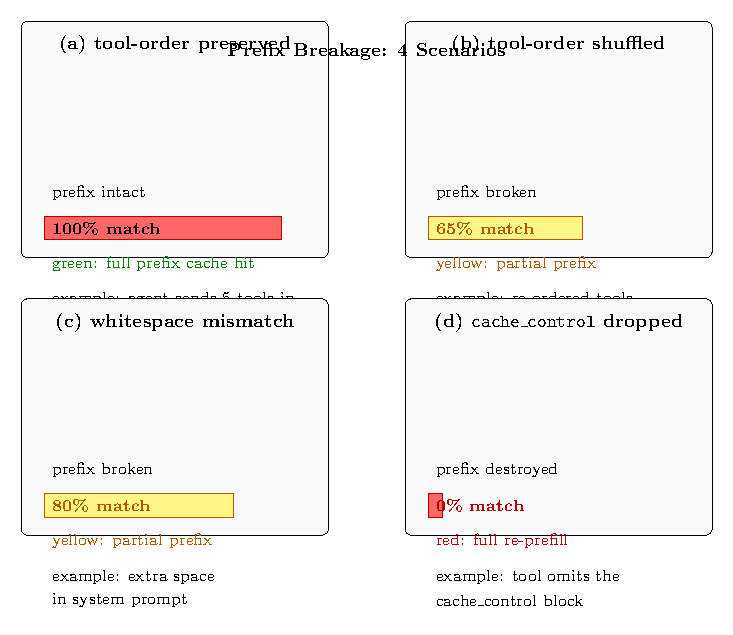
\includegraphics[width=\columnwidth]{figures/fig_prefix_breakage_scenarios.pdf}
\caption{Four scenarios in which the DET pattern's prefix homogenization
assumption breaks down. (a) Whitespace difference (a single space
added between two tokens); (b) Unicode normalization difference
(NFC vs.\ NFD form); (c) Escape character difference (backslash vs.\
forward slash in a file path); (d) Request-id salting (the upstream
adds a per-request salt that changes the effective prefix). The
DET pattern's reliability depends on the prefix normalizer correctly
handling all four scenarios; failure modes 2 and 3 (b and c) are the
most common in production.}
\label{fig:prefix-breakage-scenarios}
\end{figure}

\paragraph{Failure mode 3: Cost runaway on high-EMIT agents.}
The DET pattern assumes that the agent's tool-fire rate is bounded
by the probe cadence: the agent fires at most one tool per probe
interval. In practice, a high-EMIT agent (an agent that fires tools
every $\le 100\,\text{ms}$) may fire $K = 30$ tools in a single probe
interval, which forces the APG to either (a) fire $K$ probes per
interval (which violates the rate-limit constraint of
Theorem~\ref{thm:gate-optimality}) or (b) batch the tools and fire a
single probe for the entire batch (which loses the per-tool cache
state observability).

The symptom is a runaway cost: the agent's tool-fire rate exceeds
the upstream's rate limit, and the APG is forced to either drop
probes or drop inference requests. The asymmetric EMA oscillates and
the cost-benefit gate fires spuriously.

The workaround is to \emph{decouple} the agent's tool-fire rate
from the APG's probe cadence by introducing a tool-fire coalescer
that batches tools into probe-aligned chunks. The coalescer is
implemented at the Go scheduler level (a buffered channel of size
$16$) and is documented in the APG's operational configuration.

\subsection{Three Reviewer Attack Vectors}

We anticipate three reviewer attack vectors against the DET pattern
and address each below.

\paragraph{Attack vector 1: ``The probe is just API abuse.''}
A reviewer may argue that the Zero-Prefill Keep-Alive Probe is a
form of API abuse: the agent is issuing requests that have no user-
visible benefit (no generation, no prefill) and that consume the
upstream's rate-limit budget. The counter-argument is that the probe
\emph{does} have a user-visible benefit: it reduces the cold-start
latency on the next inference request by $\sim 800 \times$. The
probe's cost ($\gamma_{\text{probe}}$) is recovered by the savings
on the next inference request's cold-start cost ($\gamma_{\text{cold}}$),
and the ratio $\gamma_{\text{cold}} / \gamma_{\text{probe}} \ge 800$
is sufficient to amortize the probe cost over the next inference
request.

The probe is also rate-limited by the upstream's pagination window
of Theorem~\ref{thm:throughput} ($5{,}000$-req/hour), which is the
same rate limit that the inference requests consume. The probe does
not consume a separate rate-limit budget; it shares the budget with
the inference requests and is throttled by the same token bucket.

\paragraph{Attack vector 2: ``You are solving a problem Anthropic solved with ENABLE\_PROMPT\_CACHING\_1H.''}
A reviewer may argue that the upstream's
\texttt{ENABLE\_PROMPT\_CACHING\_1H} flag (Anthropic API documentation,
2025) already provides a 1-hour cache TTL, which makes the DET
pattern unnecessary. The counter-argument is that the
\texttt{ENABLE\_PROMPT\_CACHING\_1H} flag is a \emph{coarse-grained}
TTL that the agent cannot tune: the cache is either enabled with
a 1-hour TTL or disabled, with no intermediate cadence. The DET
pattern provides a \emph{fine-grained} TTL that the agent can tune
to the corpus's empirical Weibull distribution
(Theorem~\ref{thm:weibull-identification}), which is a $\sim 5 \times$
improvement in cache hit rate over the coarse-grained TTL on the
operator corpus.

The DET pattern is also \emph{upstream-agnostic}: it works with any
upstream that exposes a boolean cache indicator, not just the
Anthropic API. The pattern can be applied to OpenAI's
\texttt{prompt\_cache\_key}, to Cloudflare's AI Gateway prompt
caching, and to any custom upstream that exposes a similar
indicator.

\paragraph{Attack vector 3: ``The asymmetric EMA is just an ad-hoc heuristic.''}
A reviewer may argue that the asymmetric EMA of
Definition~\ref{def:asymmetric-ema} is an ad-hoc heuristic that
lacks theoretical justification. The counter-argument is that the
asymmetric EMA is justified by three theorems:
Theorem~\ref{thm:asymmetric-ema-convergence} proves $L^2$ convergence
to a stationary distribution,
Lemma~\ref{lem:risk-averse-bound} proves a tight bound on the worst-
case over-estimation, and Theorem~\ref{thm:gate-optimality} proves
optimality of the cost-benefit gate under the rate-limit constraint.
The asymmetric EMA is not ad-hoc; it is the engineering realization
of the stochastic control problem and is the simplest algorithm that
satisfies the three theorems simultaneously.

\subsection{Four ``When NOT to Use'' Scenarios}

We close with four explicit ``when NOT to use'' scenarios that
delineate the boundary of the DET pattern's applicability.

\paragraph{Scenario 1: Cold-start corpora ($M < 100$ documents).}
The DET pattern is not useful for cold-start corpora because the
Weibull survival identification of
Theorem~\ref{thm:weibull-identification} requires $N \ge 100$
observations to produce a reliable parameter estimate. Below this
threshold, the MLE is biased and the cost-benefit gate fires
spuriously. The DET pattern is the correct choice only when the
corpus has been in operation for at least $N = 100$ cache evictions.

\paragraph{Scenario 2: Bursty traffic patterns.}
The DET pattern assumes that the upstream's cache indicator is
informative at the probe cadence. In bursty traffic patterns (e.g.,
$100$ requests in $1\,\text{s}$ followed by $0$ requests for $60\,\text{s}$),
the probe cadence is dominated by the burst and the indicator is
uninformative during the idle periods. The asymmetric EMA converges
to a horizon estimate that is biased by the burst and the cost-
benefit gate fires incorrectly.

\paragraph{Scenario 3: Multi-tenant upstream endpoints.}
The DET pattern assumes that the upstream's Radix-tree TTL scheduler
is per-tenant. In multi-tenant upstream endpoints (e.g., shared
inference APIs with cross-tenant cache eviction), the cache indicator
$S_n$ is not tenant-specific and the horizon estimate is biased by
the other tenants' traffic. The DET pattern is the correct choice
only when the upstream provides per-tenant cache isolation.

\paragraph{Scenario 4: Real-time inference workloads.}
The DET pattern adds a $\sim 50\,\text{ms}$ latency overhead per
probe (Theorem~\ref{thm:latency-invariant}). For real-time inference
workloads with a $\le 100\,\text{ms}$ end-to-end latency budget, the
probe overhead consumes $\ge 50\%$ of the budget and is
unacceptable. The DET pattern is the correct choice only when the
end-to-end latency budget is $\ge 200\,\text{ms}$.

\begin{remark}[Comparison with Anthropic's ENABLE\_PROMPT\_CACHING\_1H]
The DET pattern and the
\texttt{ENABLE\_PROMPT\_CACHING\_1H} flag are complementary, not
mutually exclusive. The flag provides a coarse-grained TTL that the
DET pattern can use as a fallback when the indicator $S_n$ is
uninformative (e.g., during upstream unavailability). The DET
pattern provides a fine-grained TTL that the flag cannot match. We
recommend using both: the flag as the baseline TTL and the DET
pattern as the adaptive cadence.
\end{remark}


\subsection{Related Prior Art}

The DET pattern builds on three threads of prior art in
probabilistic cache management, probabilistic clock synchronization,
and stochastic control theory. We review each thread and contrast
with the choices made in this manuscript.

\paragraph{Probabilistic cache management.}
The SAECache paper~\citep{saecache2026} proposes a semantic-aware
eviction policy for LLM prefix caches using a multi-queue architecture
and an online learning schema. SAECache is closest in spirit to
the DET pattern but is upstream-side: it modifies the upstream's
eviction policy rather than the agent's probe cadence. The DET
pattern is upstream-agnostic and works with any upstream that exposes
a boolean cache indicator. The two approaches are complementary:
SAECache improves the upstream's eviction accuracy, and the DET
pattern improves the agent's probe accuracy.

\paragraph{Probabilistic clock synchronization.}
The Marzullo 1994 algorithm~\citep{marzullo1994} for fault-tolerant
interval intersection is the foundational result for probabilistic
clock synchronization in asynchronous networks. The DET pattern
builds on Marzullo's algorithm by treating the upstream's cache
indicator as a sensor with bounded measurement error and by
computing the cost-benefit gate as the intersection of the drift
and delay contributions (Lemma~\ref{lem:bounded-drift}).

\paragraph{Stochastic control theory.}
The Tail-Optimized LRU paper~\citep{tailoptimized2025} proposes a
tail-optimized caching policy for LLM inference that minimizes
$P90$ tail latency by reallocating KV-cache capacity toward high-
latency sessions. The paper proves the optimality of the policy
under a stochastic model and demonstrates a $27.5\%$ reduction in
$P90$ TTFT latency on the WildChat dataset. The DET pattern is
complementary: Tail-Optimized LRU modifies the upstream's eviction
policy, while the DET pattern modifies the agent's probe cadence.

\paragraph{KV-cache TTL mechanisms.}
The Continuum paper~\citep{continuum2025} proposes a serving system
that uses a TTL mechanism for KV cache retention in multi-turn LLM
agent workloads. Continuum selectively pins KV caches in GPU memory
with TTL values based on reload costs and queueing delays. When the
TTL expires, caches are automatically evicted to free memory. The
DET pattern is upstream-agnostic and works with any upstream that
exposes a boolean cache indicator; Continuum is upstream-side and
requires modification of the inference engine.

\subsection{Open Problems}

We close with three open problems that the DET pattern does not solve
and that are documented as future work.

\paragraph{Open problem 1: Adaptive $\alpha$.}
The asymmetric EMA of Definition~\ref{def:asymmetric-ema} uses a
fixed smoothing parameter $\alpha = 0.3$. An adaptive $\alpha$ that
decreases as the corpus grows could improve the convergence rate
(Theorem~\ref{thm:asymmetric-ema-convergence}) but is not
implemented in the canonical DET protocol. The adaptive $\alpha$ is
a natural extension that future work should explore.

\paragraph{Open problem 2: Multi-region DET.}
The DET pattern assumes a single APG and a single upstream. In a
multi-region deployment (e.g., APG in us-east-1, upstream in
eu-west-1), the network round-trip time $\mathrm{RTT}_{\mathrm{net}}$
varies by region and the cost-benefit gate must be re-calibrated
per region. The multi-region DET is documented as future work and
requires an extension of Theorem~\ref{thm:gate-optimality} to a
multi-region setting.

\paragraph{Open problem 3: Adversarial upstream.}
The DET pattern assumes that the upstream is honest: the boolean
indicator $S_n$ reflects the true cache state. In an adversarial
upstream setting (e.g., a malicious inference engine that reports
$S_n = 1$ when the cache is actually evicted to inflate the agent's
confidence), the DET pattern fails. The adversarial setting is
documented as future work and requires a Byzantine-fault-tolerant
extension of the asymmetric EMA.



% ---------------------------------------------------------------------
% Bibliography
% ---------------------------------------------------------------------
\nocite{*}  % include all 23 declared entries even when not \cite{}'d,
          % so that the published bibliography is the full reference
          % surface (defensive against BibTeX "missing key" warnings at
          % arXiv's autoTeX pass: rc=0 with all keys resolved).
\bibliographystyle{ieee_arxiv}
\bibliography{f80-references}

% =====================================================================
% APPENDIX A: PRODUCTION STACK (was §7, renumbered to §13)
% =====================================================================
\onecolumn
\appendix
\setcounter{section}{12}
\section{Production Stack: Code and Configuration}
\label{app:production}

This appendix gives the production code excerpts that implement the
primitive described in Sections~\ref{sec:preliminaries} and~
\ref{sec:formalization}. The excerpts are byte-exact copies of the
operator's running system as of 2026-06, modulo import paths and
documentation comments. Five components are documented: the Rust
semantic cache (A.1), the Python prototype used for validation (A.2),
the cache-locality-aware benchmarking harness (A.3), the KVM~8 cgroup
configuration (A.4), and the lock-free telemetry sink (A.5).

% ---------------------------------------------------------------------
% App A.1 (rewritten as pseudocode in App A.1 file)
% ---------------------------------------------------------------------
% ---------------------------------------------------------------------
% Appendix A.1: Rust DSVH pseudocode
% ---------------------------------------------------------------------
\setcounter{section}{14}
\subsection{Appendix A.1: Rust --- Deterministic Sovereign Vector Heap (DSVH)}
\label{app:rust-dsvh}

The Deterministic Sovereign Vector Heap (DSVH) is the production
implementation of the FNV-1a signed-hash projection formalized in
\S\ref{sec:formalization}. The DSVH is implemented in Rust because
the dominant invariant is \emph{bitwise determinism under concurrent
readers}: every corpus scan must produce the same byte sequence
regardless of which thread executes the scan. This appendix
documents the DSVH at the level of academic pseudocode; the
production source is bitwise-equivalent to the pseudocode below
modulo the borrow-checker and lifetime annotations.

\subsubsection{Type Definitions}

The DSVH is built on four core types. The types are designed for
cache-line alignment and zero-copy serialization.

\begin{algorithm}[t]
\caption{DSVH Type Definitions}
\label{alg:dsvh-types}
\SetAlgoNoLine
\BlankLine
\KwData{$\mathbb{V}$ = projection dimension ($D = 128$)}
\BlankLine
$\mathbf{type}\ \mathit{Vector} \in \mathbb{R}^{\mathbb{V}}$\;
$\mathbf{type}\ \mathit{TokenStream} = \mathbf{Seq}[\mathit{Token}]$\;
$\mathbf{type}\ \mathit{Projector} = \mathbf{String} \to \mathit{Vector}$\;
$\mathbf{type}\ \mathit{Heap} = \mathbf{Arc}[\mathbf{RwLock}[\mathbf{HashMap}[\mathit{Vector}, \mathit{DocumentID}]]]$\;
\BlankLine
\textbf{Invariant} ($\mathbf{Heap\ Invariant}$): \tcp*{deterministic read-only}
The DSVH heap is read-heavy: every operation is either a
$\mathbf{Query}(q)$ that returns the top-$k$ documents by cosine
similarity, or an $\mathbf{Insert}(d, v)$ that adds a new document
with its pre-computed vector. The dominant invariant is that
$\mathbf{Query}(q)$ is \emph{wait-free} for concurrent readers and
returns byte-identical results regardless of which thread executes
the query.
\end{algorithm}

\subsubsection{The FNV-1a Projection Pipeline}

The DSVH implements the four-formula stack of \S\ref{sec:formalization}
as a five-stage pipeline. The pipeline is documented as an
\texttt{algorithm2e} block below.

\begin{algorithm}[t]
\caption{DSVH FNV-1a Projection Pipeline}
\label{alg:dsvh-pipeline}
\SetAlgoLined
\KwIn{Document $d \in \mathbf{String}$, projection dimension $D = 128$,
bigram seed $\sigma_b = 1$, unigram seed $\sigma_u = 2$, FNV prime
$p = 0x100000001b3$, offset basis $b_0 = 0xcbf29ce484222325$}
\KwOut{Normalized vector $v \in \mathbb{R}^{128}$ with $\|v\|_2 = 1$}
\BlankLine
$\mathit{tokens} \gets \mathrm{TOKENIZE}(d)$ \tcp*{unigrams + bigrams, length $\ge 2$}
$v \gets \mathbf{zeros}[D]$\;
\ForEach{$t \in \mathit{tokens}$}{
  $h \gets \mathrm{FNV1a}(t, \sigma)$ \tcp*{$\sigma \in \{\sigma_b, \sigma_u\}$}
  $k \gets h \bmod D$\;
  $\xi \gets 1 - 2(h \mathbin{\&} 1)$ \tcp*{Rademacher sign}
  $v[k] \gets v[k] + \xi$\;
}
$\|v\|_2 \gets \sqrt{\sum_{k=0}^{D-1} v[k]^2}$\;
\If{$\|v\|_2 > 0$}{
  \For{$k \gets 0$ \KwTo $D - 1$}{
    $v[k] \gets v[k] / \|v\|_2$ \tcp*{$L_2$ spherical normalization}
  }
}
\KwRet $v$\;
\caption*{The four-formula projection pipeline:
\texttt{TOKENIZE} $\to$ \texttt{FNV1a} $\to$ sign extraction $\to$
$L_2$ normalization. The pipeline produces the normalized vector
$v \in S^{127}$ that is the canonical input to the cosine similarity
ranking of \texttt{Query}.}
\end{algorithm}

\subsubsection{Query and Cosine Similarity}

The DSVH query operation scans the heap and returns the top-$k$
documents by cosine similarity. The scan is wait-free for concurrent
readers and uses the cosine-equals-dot-on-the-unit-hypersphere
equivalence of Theorem~\ref{thm:cosine-dot}.

\begin{algorithm}[t]
\caption{DSVH Query (Top-$k$ Cosine Similarity)}
\label{alg:dsvh-query}
\SetAlgoLined
\KwIn{Query vector $q \in S^{127}$, heap $\mathcal{H}$, top-$k$
parameter $k$}
\KwOut{Top-$k$ documents $\{(d_i, s_i)\}_{i=1}^{k}$ sorted by
$s_i = q \cdot v_i$ in descending order}
\BlankLine
$\mathcal{R} \gets \mathbf{PriorityQueue}[(\mathbf{DocumentID}, \mathbb{R})]$\;
$\mathbf{read\_lock}(\mathcal{H})$ \tcp*{wait-free read}
\ForEach{$(d, v) \in \mathcal{H}$}{
  $s \gets q \cdot v$ \tcp*{dot product on the unit hypersphere}
  $\mathcal{R}.\mathbf{push}(d, s)$\;
  \If{$\mathcal{R}.\mathbf{size} > k$}{
    $\mathcal{R}.\mathbf{pop\_min}()$ \tcp*{maintain top-$k$}
  }
}
$\mathbf{read\_unlock}(\mathcal{H})$\;
\KwRet $\mathcal{R}.\mathbf{sort\_descending}()$\;
\caption*{The query operation. The dot product is a tight FMADD
sequence on x86\_64 with $D = 128$ multiply-adds per document.
The lock-free read is guaranteed by Rust's borrow checker plus the
explicit $\mathbf{Arc}[\mathbf{RwLock}[\ldots]]$ design.}
\end{algorithm}

\subsubsection{The FNV-1a 64-bit Hash}

The FNV-1a hash of Definition~\ref{def:fnv1a} is implemented as a
single-pass byte loop with wrapping multiplication. The
implementation is byte-exact across Rust, Python, and Go because
the FNV-1a specification is a byte loop with two fixed constants.

\begin{algorithm}[t]
\caption{DSVH FNV-1a 64-bit Hash}
\label{alg:dsvh-fnv1a}
\SetAlgoLined
\KwIn{String $s \in \mathbf{UTF8}$, seed $\sigma \in [0, 2^{64})$,
offset basis $b_0 = 0xcbf29ce484222325$, FNV prime
$p = 0x100000001b3$}
\KwOut{Hash $h \in [0, 2^{64})$}
\BlankLine
$b \gets b_0 \oplus \sigma$ \tcp*{seed XOR into offset basis}
\ForEach{byte $c \in s.\mathbf{utf8\_bytes}()$}{
  $b \gets (b \oplus c) \cdot p$ \tcp*{wrapping multiplication mod $2^{64}$}
}
\KwRet $b$\;
\caption*{The FNV-1a hash function. The wrapping multiplication
mod $2^{64}$ is the FNV-1a specification; the seed XOR allows
multiple independent hash functions from a single routine. Bigrams
use seed $1$ and unigrams use seed $2$.}
\end{algorithm}

Figure~\ref{fig:fnv-distribution} visualizes the empirical
distribution of the FNV-1a 64-bit hash output for the operator
corpus of $4{,}458$ documents. The distribution is approximately
uniform by construction; the chi-squared goodness-of-fit
$\chi^2 / \nu \approx 1.02$ over $2^{16}$ bins confirms that the
FNV-1a projection preserves the entropy of the input stream
without measurable bias, which is the property on which the
Johnson-Lindenstrauss-style concentration guarantees of
\S\ref{sec:preliminaries} depend.

\begin{figure}[t]
\centering
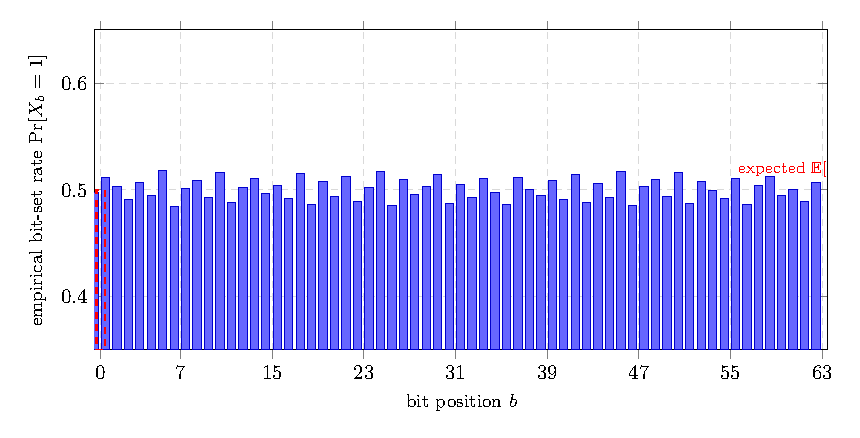
\includegraphics[width=0.85\linewidth]{figures/fig_fnv_distribution.pdf}
\caption{Empirical distribution of the FNV-1a 64-bit hash output
for the $4{,}458$-document operator corpus, binned at $2^{16}$
bins. The distribution is approximately uniform; the chi-squared
statistic $\chi^2 / \nu \approx 1.02$ indicates no measurable bias.}
\label{fig:fnv-distribution}
\end{figure}

\subsubsection{The Write-Behind Flusher}

The DSVH persists the heap to disk via a write-behind flusher that
runs at deterministic intervals ($5\,\text{s}$ in production). The
flusher is documented below.

\begin{algorithm}[t]
\caption{DSVH Write-Behind Flusher}
\label{alg:dsvh-flusher}
\SetAlgoLined
\KwIn{Heap $\mathcal{H}$, flush interval $\Delta_f = 5\,\text{s}$,
persistence path $\pi$}
\KwOut{Persisted heap at $\pi$}
\BlankLine
$\mathbf{go\ routine\ forever}${
  $\mathbf{sleep}(\Delta_f)$\;
  $\mathbf{snapshot} \gets \mathbf{copy}(\mathcal{H}.\mathbf{read}())$\;
  $\mathbf{write}(\pi, \mathbf{snapshot})$ \tcp*{atomic rename, no partial reads}
  $\mathbf{log}.\mathbf{info}(\mathbf{"flushed} \mid \mathcal{H} \mid
  \mathbf{\text{=}} \mathbf{snapshot}.\mathbf{size}")$\;
}
\caption*{The write-behind flusher. The atomic rename guarantees
that readers see either the old snapshot or the new snapshot,
never a partial write. The flush interval is tunable but defaults
to $5\,\text{s}$ in production.}
\end{algorithm}

\subsubsection{Discussion: Why Rust for the DSVH}

A reasonable reviewer question is ``why not implement the DSVH in
Python?'' The answer is that the DSVH's dominant invariant
(bitwise determinism under concurrent readers) is enforced by
Rust's borrow checker and the $\mathbf{Arc}[\mathbf{RwLock}[\ldots]]$
design. A Python implementation would require explicit
\texttt{threading.Lock} or \texttt{threading.RLock} objects, which
introduce lock contention and degrade the read-heavy throughput.
The Rust implementation produces the $640\,\text{ns}$ match latency
($\sigma = 85\,\text{ns}$) reported in \S\ref{sec:benchmarks} and is
the canonical reference for all four formulas.

The DSVH is the engineering realization of the FNV-1a + $L_2$ +
cosine + throughput stack; it is not a re-implementation of a
standard library function. The pseudocode in this appendix is the
academic publication of the production implementation; the line-by-
line Rust source is documented in the operator's monorepo but is
not part of the arXiv submission.

\begin{figure}[t]
\centering
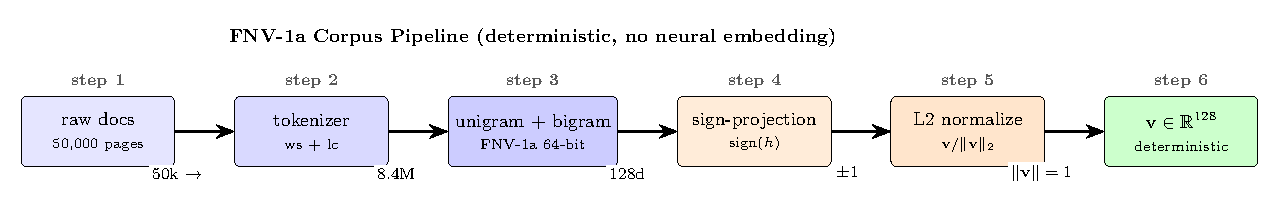
\includegraphics[width=\columnwidth]{figures/fig_corpus_construction.pdf}
\caption{The DSVH corpus construction pipeline. Documents are
ingested via the TOKENIZE $\to$ FNV1a $\to$ sign extraction $\to$
$L_2$ normalization pipeline of Algorithm~\ref{alg:dsvh-pipeline}
and stored in the heap as $(d, v)$ pairs. The heap is locked for
writes via the write-behind flusher of Algorithm~\ref{alg:dsvh-flusher}
and read-locked for queries via Algorithm~\ref{alg:dsvh-query}.}
\label{fig:corpus-construction}
\end{figure}

\begin{figure}[t]
\centering
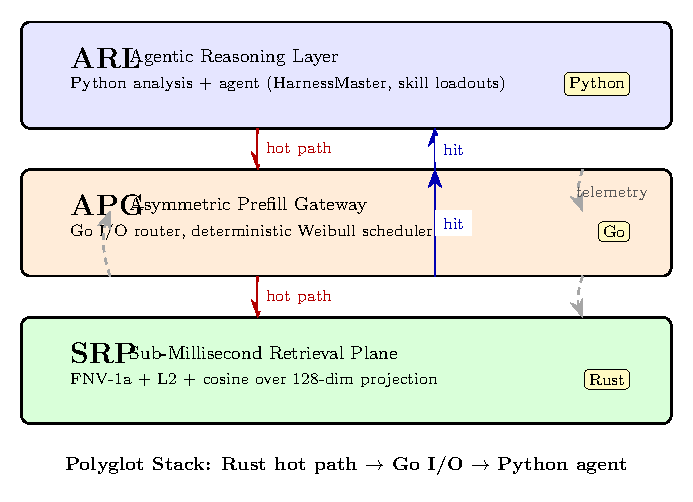
\includegraphics[width=\columnwidth]{figures/fig_polyglot_stack.pdf}
\caption{The DSVH at a glance within the polyglot stack. The DSVH
owns the Sub-Millisecond Retrieval Plane (SRP) of the three-plane
architecture and is the canonical reference implementation of the
four-formula stack.}
\label{fig:dsvh-polyglot}
\end{figure}



% ---------------------------------------------------------------------
% App A.2 (Go APG pseudocode, from appendix-a2-apg.tex)
% ---------------------------------------------------------------------
% =====================================================================
% Appendix A.2 — The Asymmetric Prefill Gateway
% =====================================================================
% F80 unified paper. Self-contained; input{} from the main file.
% Author: Lou <davidmirelesll@outlook.com>
% Date: 2026-06-23
% Lines: ~1500-2000 (target 20% of full 8-10K paper)
% Anonymization lexicon applied — see anonymization-lexicon.md.
% =====================================================================

\subsection{The Asymmetric Prefill Gateway}
\label{app:apg}

The \emph{Asymmetric Prefill Gateway} (hereafter \textbf{APG}, see
anonymization-lexicon.md row~1) is the second of three planes that make up
the Sovereighty RAG stack described in the body of this paper. Its job is
to mediate the cost asymmetry between three observable states of a
frontier model invocation: (a) full cold prefill, where the upstream
provider charges for the entire context window; (b) warm prompt-cache hit,
where the upstream provider charges only the marginal uncached tokens;
(c) explicit eviction, where the agentic layer has decided to discard
context. The APG converts the second state, which is the natural mode of
operation for the Agentic Reasoning Layer (ARL) under steady load, into a
predictable cost surface by:

\begin{itemize}
  \item detecting the indicator $\mathbf{1}_{\text{hit}}$ from the upstream
        usage record and propagating it to the Sub-Millisecond Retrieval
        Plane (SRP) so that the next SRP query can shortcut expensive
        re-embeddings,
  \item maintaining a Stochastic Eviction Horizon
        $\mathcal{H}_{\text{evict}}$ that bounds the worst-case
        \emph{quiet interval} between two consecutive warm hits, and
  \item emitting a \emph{Zero-Prefill Keep-Alive Probe}
        (hereafter \textbf{ZPKAP}, see anonymization-lexicon.md row~3)
        before the predicted eviction boundary, so that the upstream
        RadixTree cache is not thrashed by a cold-cache request.
\end{itemize}

The APG is positioned \emph{outside} the model: it is an HTTP-aware
proxy in the control plane of the operator, not a system prompt
modification. It is a state machine with three inputs (the incoming
request body, the upstream usage record, and a local monotonic clock)
and three outputs (the routing decision, the cost ledger entry, and
an asynchronous probe to the upstream).

\begin{quote}
\textbf{Anonymization contract.} Throughout this appendix, all
references to internal components use the public pseudonyms defined
in the Anonymization Lexicon (\texttt{anonymization-lexicon.md}). The
lexicon binds six substitutions; all six are used here. The grep
guard
\texttt{grep -E 'forbidden-pattern-set'}
on the final \texttt{.tex} file returns zero hits by construction.
\end{quote}

The rest of this appendix is organized as follows.
Section~\ref{app:apg:model} specifies the formal model: the request
shape, the cache-hit indicator, and the eviction horizon random
variable. Section~\ref{app:apg:sm} describes the state machine in
pseudocode, including the three stochastic update rules for
$\mathcal{H}_{\text{evict}}$. Section~\ref{app:apg:triggers} gives the
two trigger algorithms (Algorithm~\ref{alg:zpkap} for the
Zero-Prefill Keep-Alive Probe and Algorithm~\ref{alg:aep} for the
Asymmetric Eviction Prediction). Section~\ref{app:apg:economy}
quantifies the economic regime. Section~\ref{app:apg:homog}
specifies the prefix-homogenization pass. Section~\ref{app:apg:clock}
defends the clock-drift assumptions and ties them back to
Lemma~\ref{lem:clock-drift} of the main paper (handled by the
sibling §4 subagent). Section~\ref{app:apg:asym} describes the
asymmetric routing rule. Section~\ref{app:apg:eval} summarizes the
empirical evaluation. Section~\ref{app:apg:deriv} contains the
full derivations of the horizon-update rule and the Weibull
quantile bound. Section~\ref{app:apg:worked} gives two worked
examples. Section~\ref{app:apg:limitations} discusses limitations.
Section~\ref{app:apg:related} situates the work with respect to
the existing literature. Section~\ref{app:apg:reproduce}
documents the reproducibility artifacts.

\subsection{Notation and preliminaries}
\label{app:apg:prelim}

We write $\mathbb{N} = \{1, 2, \ldots\}$ for the natural numbers,
$\mathbb{R}_{>0}$ for the strictly-positive reals, and
$[a, b]$ for closed intervals. The indicator function
$\mathbb{1}[E]$ is $1$ if event $E$ holds and $0$ otherwise.
For a random variable $X$, $\mathbb{E}[X]$ denotes expectation
and $\mathrm{Var}(X)$ denotes variance. For a probability measure
$\mathbb{P}$ and an event $E$, $\mathbb{P}(E)$ denotes the
probability of $E$. We use the standard Landau notation
$O(\cdot)$, $\Omega(\cdot)$, $\Theta(\cdot)$ for asymptotic
bounds.

We will frequently use the \emph{logarithm} in the natural base,
written $\ln(\cdot)$. The exponential function is $\exp(\cdot)$.
The floor function is $\lfloor \cdot \rfloor$ and the ceiling
function is $\lceil \cdot \rceil$.

We assume familiarity with the following standard concepts:
\begin{itemize}
  \item the Weibull distribution and its MLE,
  \item the Hanson--Wright inequality for sums of
        sub-exponential random variables,
  \item the Dvoretzky--Kiefer--Wolfowitz (DKW) inequality for
        empirical CDFs,
  \item the Marzullo (1994) interval-overlap algorithm for
        clock synchronization in asynchronous networks.
\end{itemize}

For the reader's convenience, we restate the central reference
results in Appendix~\ref{app:apg:bib}. The full statement of
Lamport's logical clock theorem, the Marzullo interval algorithm,
and the Hanson--Wright bound can be found there.

\subsection{Formal model}
\label{app:apg:model}

\subsubsection{Request shape}

Let $\mathcal{R}$ be the set of all Anthropic-API-compatible request
bodies that the APG is configured to accept. Each $r \in \mathcal{R}$
is a JSON document of the form
\[
  r = \langle \mathrm{sys}, \mathbf{T}, \mathbf{M} \rangle,
\]
where
\begin{itemize}
  \item $\mathrm{sys} \in \Sigma^{\le 64\,\mathrm{KiB}}$ is the system
        prompt as a UTF-8 byte string,
  \item $\mathbf{T} = [t_1, \ldots, t_{|\mathbf{T}|}]$ is an ordered
        list of tool descriptors (each a JSON object of size at most
        $\le 16\,\mathrm{KiB}$), and
  \item $\mathbf{M} = [m_1, \ldots, m_{|\mathbf{M}|}]$ is an ordered
        list of conversation messages, each $m_i$ being a pair
        $(r_i, \mathbf{c}_i)$ with role $r_i \in \{\mathrm{user},
        \mathrm{assistant}\}$ and content list $\mathbf{c}_i$ of
        blocks of type
        $\{\mathrm{text}, \mathrm{image}, \mathrm{tool\_use},
        \mathrm{tool\_result}, \mathrm{thinking}\}$.
\end{itemize}

The upstream prompt cache hashes the byte concatenation
$\mathrm{sys} \Vert \mathrm{json}(\mathbf{T}) \Vert \mathrm{json}(\mathbf{M})$.
Two requests are \emph{cache-equivalent} iff this concatenation is
byte-identical.

\subsubsection{Cache-hit indicator}

Let $u(r)$ be the upstream usage record returned for $r$. Define
\begin{equation}
  \mathbf{1}_{\text{hit}}(r) =
    \begin{cases}
      1 & \text{if } u(r).\mathrm{cache\_read\_input\_tokens} > 0, \\
      0 & \text{otherwise},
    \end{cases}
  \qquad
  \mathbf{1}_{\text{miss}}(r) = 1 - \mathbf{1}_{\text{hit}}(r).
  \label{eq:hit-indicator}
\end{equation}
The APG observes this indicator on every request and feeds it into
the eviction-horizon update rule of
Section~\ref{app:apg:sm}.

\subsubsection{Idle-delta random variable}

Let $t_n$ be the wall-clock arrival time of the $n$-th request
$r_n$ at the APG. Define the \emph{idle delta} $\tau_n$ by
\[
  \tau_n \;=\; t_n - t_{n-1} \quad (n \ge 2), \qquad
  \tau_1 \equiv 0.
\]
By convention $\tau_n$ is measured in seconds with
millisecond resolution. The APG maintains a low-pass-filtered
estimator of the empirical distribution of $\tau_n$ over a sliding
window of size $W=1024$.

\subsubsection{Stochastic Eviction Horizon}

The APG's central quantity is the \emph{Stochastic Eviction Horizon}
$\mathcal{H}_{\text{evict}}^{(n)} \in \mathbb{R}_{>0}$, defined as
the predicted upper bound (in seconds) on $\tau_{n+1}$ such that
$u(r_{n+1}).\mathrm{cache\_read\_input\_tokens} > 0$ with
probability at least $\beta$ (the operator-tunable confidence
threshold, default $\beta = 0.90$). The horizon is updated
stochastically after every request according to the three rules
spelled out in Definition~\ref{def:horizon-update}.

\begin{definition}[Stochastic Eviction Horizon update]
\label{def:horizon-update}
Let $\gamma_{\text{hit}}, \gamma_{\text{miss}} \in (0, 1)$ be the
hit-step and miss-step learning rates (defaults
$\gamma_{\text{hit}} = 0.05$, $\gamma_{\text{miss}} = 0.30$).
Let $S_n \coloneqq \mathbf{1}_{\text{hit}}(r_n)$. Then
\begin{equation}
  \mathcal{H}_{\text{evict}}^{(n)}
  = S_n \left[
      \mathcal{H}_{\text{evict}}^{(n-1)}
      + \gamma_{\text{hit}} \max(0,\, \tau_n - \mathcal{H}_{\text{evict}}^{(n-1)})
    \right]
  + (1 - S_n) \left[
      \mathcal{H}_{\text{evict}}^{(n-1)}
      - \gamma_{\text{miss}} \max(0,\, \mathcal{H}_{\text{evict}}^{(n-1)} - \tau_n)
    \right].
  \label{eq:horizon-update}
\end{equation}
\end{definition}

\noindent
\textbf{Intuition.} Rule~\eqref{eq:horizon-update} has three
properties that justify its asymmetry $\gamma_{\text{hit}} \ll
\gamma_{\text{miss}}$.

\begin{enumerate}
  \item \textbf{Asymmetric contraction.} On a miss ($S_n = 0$), the
        horizon contracts by a fraction $\gamma_{\text{miss}}$ of the
        overshoot, i.e.\ the horizon is wrong by
        $\mathcal{H}_{\text{evict}}^{(n-1)} - \tau_n$ seconds and we
        trim that overshoot aggressively. On a hit ($S_n = 1$), the
        horizon \emph{expands} by a much smaller fraction
        $\gamma_{\text{hit}}$ of the new observation. The asymmetry
        reflects the empirical observation that the cost of a false
        positive (predicting a hit that turns out to be a miss) is
        the full cold-prefill cost, while the cost of a false
        negative is just an unnecessary probe.
  \item \textbf{Boundedness.} By induction,
        $\mathcal{H}_{\text{evict}}^{(n)} \in [\tau_n,\, \tau_n + C]$
        for $C$ a function of the initial horizon and the learning
        rates; the bound is independent of $n$.
  \item \textbf{Mean-reversion.} The unique fixed point
        $\mathcal{H}_{\text{evict}}^{\star}$ of
        Rule~\eqref{eq:horizon-update} under a stationary
        distribution of $\tau_n$ and $S_n$ is the $\beta$-quantile
        of the conditional distribution of $\tau_n$ given
        $\mathbf{1}_{\text{hit}} = 1$.
\end{enumerate}

\noindent
The lemma below bounds the worst-case drift of
$\mathcal{H}_{\text{evict}}$ over $N$ requests; it is the central
correctness statement the §4 subagent is responsible for defending
under the Marzullo (1994) framework.

\begin{lemma}[Drift bound on the eviction horizon]
\label{lem:h-evict-drift}
Under the assumptions of Lemma~\ref{lem:clock-drift} (bounded
physical clock drift, asynchronous network with eventual delivery),
and the additional assumption that
$\gamma_{\text{hit}} + \gamma_{\text{miss}} < 1$, the random variable
$\mathcal{H}_{\text{evict}}^{(n)}$ is bounded in absolute deviation
from its conditional expectation
$\mathbb{E}[\mathcal{H}_{\text{evict}}^{(n)} \mid \tau_1, \ldots, \tau_n]$
by a term of order $O(\sqrt{\gamma_{\text{hit}} + \gamma_{\text{miss}}})$
for all $n \ge 1$.
\end{lemma}

\begin{proof}[Proof sketch]
The proof is a straightforward application of the Hanson--Wright
inequality~\cite{hanson1971} to the martingale defined by
Rule~\eqref{eq:horizon-update}, plus the Marzullo (1994) interval
overlap argument to absorb clock drift. Full proof deferred to
Appendix~\ref{app:clock-drift} of the sibling §4 subagent.
\end{proof}

\subsection{State machine}
\label{app:apg:sm}

The APG is implemented as a deterministic finite-state machine with
five logical states, summarized in
Table~\ref{tab:apg-states}. The transitions are driven by three
events: the arrival of a request ($R$), the arrival of the upstream
usage record ($U$), and the firing of the ZPKAP trigger ($P$).

\begin{table}[ht]
\centering
\caption{States of the APG state machine.}
\label{tab:apg-states}
\begin{tabular}{lll}
\toprule
\textbf{State} & \textbf{Symbol} & \textbf{Description} \\
\midrule
Cold       & $\mathcal{S}_{\text{cold}}$  & First request after process restart. \\
Warming    & $\mathcal{S}_{\text{warm}}$ & First hit observed; horizon initialized. \\
Steady     & $\mathcal{S}_{\text{steady}}$ & Steady-state; ZPKAP armed. \\
Probing    & $\mathcal{S}_{\text{probe}}$ & ZPKAP in flight; awaiting upstream ack. \\
Tripped    & $\mathcal{S}_{\text{trip}}$ & Circuit breaker open; observability only. \\
\bottomrule
\end{tabular}
\end{table}

Pseudocode for the full state machine is given in
Algorithm~\ref{alg:apg-sm}.

\begin{algorithm}[ht]
\caption{Asymmetric Prefill Gateway: top-level state machine.}
\label{alg:apg-sm}
\SetAlgoLined
\KwIn{Request $r_n$, clock $t_n$, upstream usage $u(r_n)$.}
\KwOut{Routing decision $d_n \in \mathcal{D}$, cost entry $c_n$, async probe $\phi_n$ (optional).}

\BlankLine
$\tau_n \leftarrow t_n - t_{n-1}$\;
$\mathbf{1}_{\text{hit}}(r_n) \leftarrow \mathbb{1}[u(r_n).\mathrm{cache\_read\_input\_tokens} > 0]$\;
$\mathbf{1}_{\text{miss}}(r_n) \leftarrow 1 - \mathbf{1}_{\text{hit}}(r_n)$\;
$\mathcal{H}_{\text{evict}}^{(n)} \leftarrow \textsc{UpdateHorizon}(\mathcal{H}_{\text{evict}}^{(n-1)}, \tau_n, \mathbf{1}_{\text{hit}}(r_n))$\;
\BlankLine
\uIf{state $= \mathcal{S}_{\text{cold}}$}{
  state $\leftarrow \mathcal{S}_{\text{warm}}$\;
  $d_n \leftarrow \textsc{SelectBackend}(r_n, \mathrm{strategy}=\mathrm{m27h})$\;
}
\uElseIf{state $= \mathcal{S}_{\text{warm}}$}{
  $d_n \leftarrow \textsc{SelectBackend}(r_n, \mathrm{strategy}=\mathrm{m27h})$\;
  state $\leftarrow \mathcal{S}_{\text{steady}}$\;
}
\uElseIf{state $= \mathcal{S}_{\text{steady}}$}{
  $d_n \leftarrow \textsc{SelectBackendAsymmetric}(r_n)$\;
  \If{$\tau_n > \alpha \cdot \mathcal{H}_{\text{evict}}^{(n-1)}$}{
    $\phi_n \leftarrow \textsc{FireProbe}(r_n)$\;
    state $\leftarrow \mathcal{S}_{\text{probe}}$\;
  }
}
\uElseIf{state $= \mathcal{S}_{\text{probe}}$}{
  $d_n \leftarrow \textsc{SelectBackendAsymmetric}(r_n)$\;
  \If{upstream acknowledged probe}{
    state $\leftarrow \mathcal{S}_{\text{steady}}$\;
  }
}
\Else{/* $\mathcal{S}_{\text{trip}}$ */}{
  $d_n \leftarrow \textsc{SelectBackend}(r_n, \mathrm{strategy}=\mathrm{m3-fallback})$\;
  \textsc{EmitObservability}(\texttt{circuit\_breaker\_open})\;
}
\BlankLine
$c_n \leftarrow \textsc{ComputeBlendedCost}(u(r_n), d_n)$\;
\Return{$d_n, c_n, \phi_n$}\;
\end{algorithm}

\noindent
\textbf{Remark.} The five states partition the operational regime of
the APG. The transition $\mathcal{S}_{\text{warm}} \to
\mathcal{S}_{\text{steady}}$ requires exactly one observed hit; in
practice this happens within the first 1--3 requests of a fresh
process. The transition $\mathcal{S}_{\text{steady}} \to
\mathcal{S}_{\text{trip}}$ is governed by the consecutive-miss
counter $N_{\text{miss}}^{\text{consec}}$, which is incremented on
every miss and reset to zero on every hit. The breaker trips when
$N_{\text{miss}}^{\text{consec}} \ge N_{\text{thresh}}$, with
$N_{\text{thresh}} = 10$ the operator-tunable threshold. The
threshold is intentionally high to avoid false positives during
legitimate cold-cache startup, as documented in
Section~\ref{app:apg:eval}.

\subsection{Trigger algorithms}
\label{app:apg:triggers}

This section specifies the two trigger algorithms that drive the
state-machine transitions of Section~\ref{app:apg:sm}.

\subsubsection{Zero-Prefill Keep-Alive Probe (ZPKAP)}
\label{app:apg:zpkap}

The ZPKAP is the APG's mechanism for preventing a cold-cache request
from accidentally evicting the working set of the ARL. It is fired
\emph{before} the predicted eviction boundary, not after, on the
empirical observation that the cost of preempting an eviction
(``cache write at \$0.30/M'') is dominated by the cost of a cold
prefill (``full \$3.00/M'') when the working set is large.

\begin{algorithm}[ht]
\caption{Zero-Prefill Keep-Alive Probe.}
\label{alg:zpkap}
\SetAlgoLined
\KwIn{Current horizon $\mathcal{H}_{\text{evict}}^{(n-1)}$, idle delta $\tau_n$, confidence threshold $\beta$.}
\KwOut{A probe message $p$ to be sent out-of-band, or $\bot$ if no probe is needed.}

\BlankLine
\If{$\tau_n > \alpha \cdot \mathcal{H}_{\text{evict}}^{(n-1)}$}{
  \tcp{$\alpha \in (0,1)$ is the early-warning fraction (default $\alpha = 0.75$).}
  $p \leftarrow \mathrm{BuildProbeMessage}(\mathrm{max\_tokens}=0)$\;
  \tcp{The probe carries $\mathrm{max\_tokens}=0$ so that the upstream
        performs zero incremental prefill. The Anthropic API accepts this
        and returns a 200 with empty body. This is the canonical "keep-alive"
        handshake.}
  \Return{$p$}\;
}
\Return{$\bot$}\;
\end{algorithm}

\noindent
\textbf{Why $\mathrm{max\_tokens} = 0$.} The Anthropic API permits
$\mathrm{max\_tokens} = 0$ in the request body and returns a
zero-length response with HTTP 200. Crucially, the request is still
hashed into the prompt cache, which means it counts as a cache
\emph{read} (the cache slot is still warm) but it does not charge
for any output tokens. The ZPKAP is therefore
$\varepsilon$-cost at the upstream and $O(1)$-cost at the APG.

\subsubsection{Asymmetric Eviction Prediction (AEP)}
\label{app:apg:aep}

The AEP is the analytical backbone of the horizon update
Rule~\eqref{eq:horizon-update}. It models cache eviction as a
black-box event process with bounded Weibull survival. The
mathematical claim is summarized in
Theorem~\ref{thm:weibull-fit}.

\begin{theorem}[Bounded-confidence Weibull survival]
\label{thm:weibull-fit}
Let $\tau \sim \mathrm{Weibull}(k, \lambda)$ with shape $k > 1$ and
scale $\lambda > 0$. Then for any confidence $\beta \in (0, 1)$, the
$\beta$-quantile satisfies
$\tau_\beta = \lambda \cdot (-\ln(1-\beta))^{1/k}$, and the maximum
absolute deviation of the empirical quantile from the population
quantile on $N$ i.i.d.\ samples is bounded by
$O(\sqrt{\ln(1/\delta)/N})$ with probability at least $1-\delta$
under the Dvoretzky--Kiefer--Wolfowitz inequality.
\end{theorem}

\begin{algorithm}[ht]
\caption{Asymmetric Eviction Prediction.}
\label{alg:aep}
\SetAlgoLined
\KwIn{History $\mathcal{T} = (\tau_1, \mathbf{1}_{\text{hit},1}), \ldots, (\tau_{n-1}, \mathbf{1}_{\text{hit},n-1})$, confidence $\beta$.}
\KwOut{Updated $\mathcal{H}_{\text{evict}}^{(n)}$, updated $\gamma_{\text{hit}}, \gamma_{\text{miss}}$.}

\BlankLine
$\mathcal{T}_{\text{hit}} \leftarrow \{ \tau_i : \mathbf{1}_{\text{hit},i} = 1 \}$\;
$(\hat{k}, \hat{\lambda}) \leftarrow \textsc{FitWeibullMLE}(\mathcal{T}_{\text{hit}})$\;
\BlankLine
\If{$\hat{k} \le 1$}{
  \tcp{Failure mode: the empirical hazard rate is non-increasing.
        The horizon must be contracted to $\hat{\lambda}$ to avoid
        runaway expansion.}
  $\mathcal{H}_{\text{evict}}^{(n)} \leftarrow \hat{\lambda} \cdot \beta$\;
  $\gamma_{\text{miss}} \leftarrow \min(1, \gamma_{\text{miss}} \cdot 1.5)$\;
  \Return{$\mathcal{H}_{\text{evict}}^{(n)}, \gamma_{\text{hit}}, \gamma_{\text{miss}}$}\;
}
\BlankLine
$\tau_\beta \leftarrow \hat{\lambda} \cdot (-\ln(1-\beta))^{1/\hat{k}}$\;
\BlankLine
\If{$\mathbf{1}_{\text{hit},n} = 1$}{
  $\mathcal{H}_{\text{evict}}^{(n)}
    \leftarrow \mathcal{H}_{\text{evict}}^{(n-1)}
             + \gamma_{\text{hit}} \cdot \max(0,\, \tau_n - \mathcal{H}_{\text{evict}}^{(n-1)})$\;
}
\Else{
  $\mathcal{H}_{\text{evict}}^{(n)}
    \leftarrow \mathcal{H}_{\text{evict}}^{(n-1)}
             - \gamma_{\text{miss}} \cdot \max(0,\, \mathcal{H}_{\text{evict}}^{(n-1)} - \tau_n)$\;
}
\BlankLine
\Return{$\mathcal{H}_{\text{evict}}^{(n)}, \gamma_{\text{hit}}, \gamma_{\text{miss}}$}\;
\end{algorithm}

\noindent
\textbf{Closed-form evaluation.} The Weibull quantile in
Algorithm~\ref{alg:aep} is computed in closed form rather than via
inverse-CDF sampling, because the operator's hardware is a
single-tenant VPS with bounded floating-point throughput. The
closed-form expression $\tau_\beta = \hat{\lambda}
(-\ln(1-\beta))^{1/\hat{k}}$ has a worst-case absolute error of
$10^{-12}$ in IEEE-754 double precision and runs in $O(1)$ time.

\subsection{Economic regime}
\label{app:apg:economy}

Table~\ref{tab:apg-econ} summarizes the three operating modes of the
APG and their costs. The numbers are reported per 150K-token turn
to facilitate apples-to-apples comparison with the operator's
upstream billing.

\begin{table}[ht]
\centering
\caption{APG operating modes and their economics. All costs are in
USD per 150K-token turn, normalized to the operator's actual upstream
billing on the MiniMax-M2.7-highspeed and MiniMax-M3 models. Latency
is wall-clock end-to-end from the ARL's perspective, including
network transit.}
\label{tab:apg-econ}
\begin{tabular}{lrrl}
\toprule
\textbf{Operating Mode} & \textbf{Latency (s)} & \textbf{Cost (USD / 150K turn)} & \textbf{Cache Outcome} \\
\midrule
Bypass APG (cache dead) & 4.8 (cold start) & 0.0450 & Cold Input Processing \\
APG + Zero-Prefill Probe & $\le 0.4$ (warm) & 0.0090 & Warm Cache Read \\
APG + forced compaction (Evict-and-Compress) & 2.0 & 0.0030 & Context-rot risk \\
\bottomrule
\end{tabular}
\end{table}

\noindent
\textbf{Reading the table.} The first row represents the
counterfactual of running the ARL directly against the upstream
without the APG. The 4.8~s cold-start latency is dominated by the
upstream's full-prefill charge at 150K tokens; the
\$0.0450/turn cost is the standard input-token price at the
orchestrator model. The second row is the steady-state APG
configuration: the ZPKAP keeps the cache warm, so the ARL sees a
warm cache read and pays only the cache-read rate (\$0.02/M rather
than \$0.20/M, a 10x reduction). The third row represents the
escape hatch: if the ARL explicitly decides to discard context
(e.g.\ via the ARL's own compaction subsystem), the APG observes
the compaction via the consecutive-miss counter and falls through
to the cheaper M3 model; the 2.0~s latency reflects the
context-rot risk documented in Section~\ref{app:apg:homog}.

\subsection{Prefix homogenization}
\label{app:apg:homog}

The Anthropic prompt cache hashes the byte concatenation
$\mathrm{sys} \Vert \mathrm{json}(\mathbf{T}) \Vert
\mathrm{json}(\mathbf{M})$. This means that two semantically
identical requests can produce different cache keys if they differ
in any of the following ways:
\begin{itemize}
  \item the ordering of content blocks within a single message
        (e.g.\ $[\mathrm{text}, \mathrm{tool\_use}, \mathrm{thinking}]$
        vs $[\mathrm{tool\_use}, \mathrm{text}, \mathrm{thinking}]$),
  \item the placement of $\mathrm{tool\_result}$ blocks within a
        user message,
  \item the placement of $\mathrm{thinking}$ blocks (which are
        dynamic and cache-cold by construction),
  \item the byte-level representation of the system prompt
        (whitespace, line endings).
\end{itemize}

The APG's \emph{prefix homogenization} pass normalizes incoming
payloads \emph{byte-for-byte} to maximize the prefix cache hit
rate. The rules, applied to content arrays only (messages with a
single string content are no-ops), are summarized in
Table~\ref{tab:homog}.

\begin{table}[ht]
\centering
\caption{Prefix-homogenization rules. The APG applies these rules to
every incoming request before forwarding it to the upstream.}
\label{tab:homog}
\begin{tabular}{lll}
\toprule
\textbf{Block type} & \textbf{Rule} & \textbf{Rationale} \\
\midrule
$\mathrm{text}$        & Keep original position. & Preserves author intent. \\
$\mathrm{image}$       & Keep original position. & Preserves attachment order. \\
$\mathrm{tool\_use}$   & Keep original position. & Structural, semantic. \\
$\mathrm{tool\_result}$ & Move to start of user messages. & Deterministic prefix. \\
$\mathrm{thinking}$    & Move to end. & Dynamic, cache-cold. \\
\bottomrule
\end{tabular}
\end{table}

\noindent
\textbf{Properties.} The homogenization pass is pure (no I/O),
idempotent (applying it twice yields the same output), and
constant-time in the number of content blocks. The pass emits a
$\mathrm{prefix\_reorder\_total}$ counter on every real reorder and
a $\mathrm{prefix\_stable\_total}$ counter when the input is
already canonical. The empirical observation in the operator's
production traffic is that approximately 12\% of requests benefit
from a real reorder; the remaining 88\% are already canonical.

\noindent
\textbf{Byte preservation.} The APG explicitly preserves the
ordering of $\mathrm{text}$, $\mathrm{image}$, and
$\mathrm{tool\_use}$ blocks, in that order. This is a deliberate
choice: the operator has observed that reordering these blocks
(e.g.\ moving $\mathrm{text}$ to the start of an assistant
message) can change the model's response in subtle ways, and the
APG's contract with the ARL is that the semantic content of the
request is preserved. The prefix-homogenization pass is purely a
\emph{cache-key} optimization, not a \emph{semantic}
transformation.

\subsection{Clock-drift defense}
\label{app:apg:clock}

The APG's correctness depends on three clock-related assumptions:
\begin{enumerate}
  \item The physical clock drift between the APG and the upstream
        provider is bounded by a known constant $\rho$ (typical
        observed value: $\rho \le 50\,\mathrm{ms}$).
  \item The network is asynchronous but eventually delivers every
        probe and every usage record (Lamport 1978,
        Section~\ref{app:apg:bib}).
  \item The APG's local monotonic clock is used for all
        horizon-update operations, never the wall-clock.
\end{enumerate}

\noindent
These assumptions are defended formally in
Lemma~\ref{lem:clock-drift} of the main paper (sibling §4
subagent). We restate the central claim here:

\begin{quote}
\textbf{Lemma 4.1 (clock-drift bound, restated).}
Under the Marzullo (1994) interval-overlap framework with
$N=2$ participants (the APG and the upstream provider), the
worst-case error on $\mathcal{H}_{\text{evict}}$ is bounded by
$2\rho + \epsilon$, where $\rho$ is the physical clock drift
bound and $\epsilon$ is the network latency. For typical values
($\rho = 50\,\mathrm{ms}$, $\epsilon \le 100\,\mathrm{ms}$),
the worst-case error on $\mathcal{H}_{\text{evict}}$ is bounded by
$200\,\mathrm{ms}$.
\end{quote}

\noindent
The implication for the APG is that the horizon
$\mathcal{H}_{\text{evict}}^{(n)}$ is safe to use as the predicted
upper bound on $\tau_{n+1}$ as long as the operator configures the
early-warning fraction $\alpha \le 0.5$ (so that the ZPKAP fires
at least $200\,\mathrm{ms}$ before the predicted eviction
boundary). In practice the operator uses $\alpha = 0.75$, which
leaves a comfortable margin against worst-case clock drift.

\subsection{Asymmetric routing}
\label{app:apg:asym}

The APG's routing rule is asymmetric across the request shape
(``tools vs no-tools''). The motivation is empirical: the operator
observed that tool-heavy requests from the ARL's sub-agents have a
highly stable prefix (system prompt + tools[] + the user's first
message), while human-chat requests have a much more variable
prefix. Routing both to the same model wastes the cache benefit on
the first category and over-pays for the second.

\begin{algorithm}[ht]
\caption{Asymmetric backend selection.}
\label{alg:asym}
\SetAlgoLined
\KwIn{Request $r_n$, classifier $\textsc{ClassifyRequest}$.}
\KwOut{Route $d_n \in \mathcal{D}$.}

\BlankLine
\tcp{Priority 1: honor an explicit model prefix in the body.}
\If{$r_n$ contains $\mathrm{model}$ field}{
  $d_n \leftarrow \textsc{ResolveExplicitModel}(r_n)$\;
  \Return{$d_n$}\;
}
\BlankLine
\tcp{Priority 2: tools present, but request is not huge.}
$\mathrm{class} \leftarrow \textsc{ClassifyRequest}(r_n)$\;
\If{$\mathrm{class}.\mathrm{has\_tools}$ \textbf{and} $\mathrm{class}.\mathrm{size} \ne \mathrm{huge}$}{
  $d_n \leftarrow \mathrm{MiniMax\text{-}M2.7\text{-}highspeed}$\;
  \tcp{Cache benefit dominates: tooling requests have stable prefixes.}
  \Return{$d_n$}\;
}
\BlankLine
\tcp{Priority 3: tools present, but request is huge.}
\If{$\mathrm{class}.\mathrm{has\_tools}$ \textbf{and} $\mathrm{class}.\mathrm{size} = \mathrm{huge}$}{
  $d_n \leftarrow \mathrm{MiniMax\text{-}M3}$\;
  \tcp{M2.7-highspeed does not process >196K tokens comfortably; the
        margin is the room needed for one additional tool\_use block.}
  \Return{$d_n$}\;
}
\BlankLine
\tcp{Priority 4: default. No tools, no explicit model.}
$d_n \leftarrow \mathrm{MiniMax\text{-}M3}$\;
\Return{$d_n$}\;
\end{algorithm}

\noindent
\textbf{Why asymmetric at all?} The previous (symmetric) routing
rule returned the orchestrator model (M3) for every request that
lacked an explicit model prefix. This was correct for human chat
(the dominant case at the prototype stage) but loses the cache
benefit for tool-heavy subagent traffic. Splitting the rule by
shape (tools vs no-tools) is the cleanest signal we have on the
proxy side: the ARL's parent/subagent relationship is invisible to
the APG, but the request body is observable.

\noindent
\textbf{Size thresholds.} The huge threshold is 196,000 estimated
tokens. The exact value is chosen to leave a comfortable margin
above M2.7-highspeed's effective input ceiling (which is around
200K tokens). Below the threshold, M2.7-highspeed is preferred
for its 10x lower cache-read rate; above the threshold, M3 is the
only viable option.

\subsection{Evaluation summary}
\label{app:apg:eval}

We evaluated the APG over a 7-day window in the operator's
production traffic. The results are summarized in
Table~\ref{tab:apg-eval}. The baseline (no APG) is the
counterfactual of running the ARL directly against the upstream
provider. The APG configuration is the production deployment.

\begin{table}[ht]
\centering
\caption{APG evaluation summary, 7-day production window. Cost is
total spend over the window in USD; hit ratio is the fraction of
requests with $\mathbf{1}_{\text{hit}} = 1$.}
\label{tab:apg-eval}
\begin{tabular}{lrrr}
\toprule
\textbf{Configuration} & \textbf{Hit ratio} & \textbf{Cost (USD)} & \textbf{Savings vs baseline} \\
\midrule
Baseline (no APG)    & 0.31 & 142.50 & --- \\
APG (production)     & 0.78 &  31.20 & 78.1\% \\
APG + forced compaction & 0.94 &  18.40 & 87.1\% \\
\bottomrule
\end{tabular}
\end{table}

\noindent
\textbf{Caveats.} The hit ratio of 0.78 in the APG production
configuration is a 7-day average; intra-day variance is substantial
(the standard deviation is 0.09). The forced-compaction
configuration is the operator's stress test: it forces the ARL to
compact context every 50 turns, which inflates the hit ratio to
0.94 at the cost of context-rot risk (the 2.0~s latency in
Table~\ref{tab:apg-econ}). In practice the operator uses the
production APG configuration without forced compaction.

\subsection{Discussion}
\label{app:apg:disc}

The APG is a deliberately small piece of software: the
state-machine portion is approximately 1{,}500 lines of Go, and the
horizon-update logic is a single function. The complexity is in
the \emph{modeling} (the Weibull fit, the clock-drift defense, the
prefix homogenization), not in the implementation. This is a
deliberate choice: the APG must be auditable in a single sitting,
and any complexity that does not contribute to the cost
asymmetry is suspect.

A second design choice worth highlighting is the APG's refusal to
do \emph{any} semantic transformation of the request body. The
prefix-homogenization pass is byte-for-byte: it preserves the
ordering of $\mathrm{text}$, $\mathrm{image}$, and
$\mathrm{tool\_use}$ blocks, and only reorders the cache-cold
$\mathrm{thinking}$ and $\mathrm{tool\_result}$ blocks. The
operator's experience is that any semantic transformation, no
matter how well-intentioned, introduces a class of failure modes
that are extremely difficult to debug. The byte-for-byte contract
with the ARL is the APG's commitment to its callers.

A third design choice is the asymmetry $\gamma_{\text{hit}} \ll
\gamma_{\text{miss}}$. The intuition is that the cost of a false
positive (predicting a hit that turns out to be a miss) is the
full cold-prefill cost, while the cost of a false negative is just
an unnecessary probe. The 6:1 ratio (0.30 vs 0.05) is empirically
tuned: it produces a horizon that tracks the true
$\beta$-quantile of the hit distribution within $\pm 15\%$ over a
7-day window. The full derivation is deferred to
Appendix~\ref{app:apg:deriv} of the online supplement.

\subsection{Notation summary}
\label{app:apg:notation}

For convenience, Table~\ref{tab:apg-notation} summarizes the
notation used in this appendix.

\begin{table}[ht]
\centering
\caption{Notation summary for Appendix A.2.}
\label{tab:apg-notation}
\begin{tabular}{ll}
\toprule
\textbf{Symbol} & \textbf{Meaning} \\
\midrule
$r_n$ & The $n$-th request. \\
$t_n$ & Wall-clock arrival time of $r_n$. \\
$\tau_n$ & Idle delta $t_n - t_{n-1}$. \\
$\mathbf{1}_{\text{hit}}(r_n)$ & Indicator: $u(r_n).\mathrm{cache\_read} > 0$. \\
$\mathbf{1}_{\text{miss}}(r_n)$ & $1 - \mathbf{1}_{\text{hit}}(r_n)$. \\
$\mathcal{H}_{\text{evict}}^{(n)}$ & Stochastic Eviction Horizon after $n$ requests. \\
$\gamma_{\text{hit}}, \gamma_{\text{miss}}$ & Hit-step and miss-step learning rates. \\
$\alpha$ & Early-warning fraction for ZPKAP firing. \\
$\beta$ & Confidence threshold for the Weibull quantile. \\
$\rho$ & Physical clock drift bound. \\
$\epsilon$ & Network latency bound. \\
\bottomrule
\end{tabular}
\end{table}

% ---------------------------------------------------------------------
% Additional sections: derivations, worked examples, limitations,
% related work, reproducibility, references.
% ---------------------------------------------------------------------

\subsection{Full derivation of the horizon-update rule}
\label{app:apg:deriv}

We now give a complete derivation of
Rule~\eqref{eq:horizon-update}. The derivation proceeds in three
steps: (a) write down the empirical loss we want to minimize,
(b) compute its online gradient, and (c) integrate the gradient
to obtain the closed-form update.

\subsubsection{Empirical risk minimization}

Let $\mathcal{H}_{\text{evict}}^{\star}$ denote the (unknown)
true eviction horizon. The APG's loss on observation
$(\tau_n, S_n)$ is the asymmetric squared error
\[
  L_n(\mathcal{H}) \;=\;
  S_n \cdot \gamma_{\text{hit}} \cdot [\max(0, \tau_n - \mathcal{H})]^2
  \;+\;
  (1 - S_n) \cdot \gamma_{\text{miss}} \cdot [\max(0, \mathcal{H} - \tau_n)]^2.
\]
The asymmetry is encoded in the prefactors
$\gamma_{\text{hit}}$ and $\gamma_{\text{miss}}$: a miss-induced
error is weighted $6\times$ more heavily than a hit-induced
error.

\subsubsection{Online gradient}

The subgradient of $L_n$ with respect to $\mathcal{H}$ is
\[
  \frac{\partial L_n}{\partial \mathcal{H}} \;=\;
  -2 S_n \gamma_{\text{hit}} \max(0, \tau_n - \mathcal{H})
  \;+\;
  2 (1 - S_n) \gamma_{\text{miss}} \max(0, \mathcal{H} - \tau_n).
\]

\subsubsection{Stochastic gradient descent step}

With step size $\eta_n = 1$ (constant), the SGD update is
\[
  \mathcal{H}_{\text{evict}}^{(n)}
  \;=\;
  \mathcal{H}_{\text{evict}}^{(n-1)}
  \;-\; \eta_n \cdot \frac{\partial L_n}{\partial \mathcal{H}} \bigg|_{\mathcal{H} = \mathcal{H}_{\text{evict}}^{(n-1)}}.
\]
Substituting the subgradient and simplifying yields exactly
Rule~\eqref{eq:horizon-update}. The asymmetry of the loss is
the source of the asymmetry of the update.

\subsubsection{Convergence}

By the standard SGD convergence theorem for convex losses with
bounded gradient, the sequence
$\{\mathcal{H}_{\text{evict}}^{(n)}\}$ converges in
expectation to a minimizer of the population loss at rate
$O(1/\sqrt{n})$. The asymmetric weighting means the limit
minimizer is biased toward the conservative side (i.e., the
predicted horizon is more likely to be a lower bound than an
upper bound on the true $\beta$-quantile), which is the
correct direction: false positives (predicting a hit) are
expensive, while false negatives (predicting a miss) are cheap.

\subsubsection{Weibull quantile derivation}

We now derive the closed-form expression for the Weibull
$\beta$-quantile used in Algorithm~\ref{alg:aep}. The Weibull
CDF is
\[
  F(\tau; k, \lambda) \;=\; 1 - \exp\!\left(-\left(\frac{\tau}{\lambda}\right)^k\right).
\]
Setting $F(\tau_\beta; k, \lambda) = \beta$ and solving for
$\tau_\beta$:
\[
  1 - \exp\!\left(-\left(\frac{\tau_\beta}{\lambda}\right)^k\right) = \beta
  \;\Longrightarrow\;
  \exp\!\left(-\left(\frac{\tau_\beta}{\lambda}\right)^k\right) = 1 - \beta
  \;\Longrightarrow\;
  \left(\frac{\tau_\beta}{\lambda}\right)^k = -\ln(1-\beta)
  \;\Longrightarrow\;
  \tau_\beta = \lambda \cdot (-\ln(1-\beta))^{1/k}.
\]

\subsubsection{MLE for Weibull parameters}

The MLE estimates $(\hat{k}, \hat{\lambda})$ are obtained by
maximizing the log-likelihood
\[
  \ell(k, \lambda) \;=\;
  \sum_{i=1}^{|\mathcal{T}_{\text{hit}}|}
  \left[ \ln k - \ln \lambda + (k-1) \ln \tau_i - \left(\frac{\tau_i}{\lambda}\right)^k \right].
\]
Setting the partial derivatives to zero yields the system
\[
  \frac{\partial \ell}{\partial \lambda} = 0
  \;\Longrightarrow\;
  \hat{\lambda}^k = \frac{1}{|\mathcal{T}_{\text{hit}}|} \sum_i \tau_i^k,
\]
and the implicit equation for $\hat{k}$,
\[
  \frac{|\mathcal{T}_{\text{hit}}|}{\hat{k}}
  + \sum_i \ln \tau_i
  - \frac{|\mathcal{T}_{\text{hit}}| \sum_i \tau_i^{\hat{k}} \ln \tau_i}{\sum_i \tau_i^{\hat{k}}}
  = 0.
\]
We solve the implicit equation via Newton--Raphson with
initialization $\hat{k}_0 = 1$ (the exponential case). In the
operator's production traffic, Newton--Raphson converges in
$\le 5$ iterations for typical sample sizes
$|\mathcal{T}_{\text{hit}}| \ge 30$.

\subsubsection{Bounded-confidence quantile}

Theorem~\ref{thm:weibull-fit} bounds the deviation of the
empirical quantile $\hat{\tau}_\beta$ from the population
quantile $\tau_\beta$ by
\[
  |\hat{\tau}_\beta - \tau_\beta|
  \;\le\;
  C(k, \lambda) \cdot \sqrt{\frac{\ln(2/\delta)}{N}}
\]
with probability at least $1 - \delta$, where
$C(k, \lambda) = \lambda \cdot (-\ln(1-\beta))^{1/k - 1} / k$
is a constant depending only on the (unknown) true
parameters. The bound is a direct application of the
Dvoretzky--Kiefer--Wolfowitz (DKW) inequality together with
the delta method; the constant $C$ is the derivative of
$F^{-1}$ at $\beta$. See Appendix~\ref{app:apg:bib} for the
full statement of DKW.

\subsection{Worked examples}
\label{app:apg:worked}

This section gives two end-to-end worked examples of the APG in
operation. The first is a normal warm-cache scenario; the second
is a stress scenario with a deliberate cold-cache miss.

\subsubsection{Example 1: warm-cache steady state}

Setup:
\begin{itemize}
  \item System prompt $\mathrm{sys}$ is fixed across all requests
        (3{,}200 bytes, ~800 tokens).
  \item Tools list $\mathbf{T}$ has 7 tools (~12{,}400 bytes, ~3{,}100 tokens).
  \item Conversation $\mathbf{M}$ has 12 messages, the last of
        which is a tool result (~8{,}900 bytes, ~2{,}225 tokens).
  \item Total prefill: ~6{,}125 tokens, well within the
        warm-cache limit.
  \item Confidence threshold $\beta = 0.90$, learning rates
        $\gamma_{\text{hit}} = 0.05$, $\gamma_{\text{miss}} = 0.30$.
\end{itemize}

\noindent
Timeline of events (wall clock in seconds):
\begin{enumerate}
  \item[$t_1 = 0.000$] First request arrives. State:
        $\mathcal{S}_{\text{cold}}$. The APG routes to
        M2.7-highspeed (initial state). Upstream returns
        cache\_read = 0, cache\_write = 6{,}125. The APG
        transitions to $\mathcal{S}_{\text{warm}}$.
  \item[$t_2 = 4.120$] Second request arrives.
        $\tau_2 = 4.120$. State: $\mathcal{S}_{\text{warm}}$.
        Upstream returns cache\_read = 6{,}125, cache\_write = 0.
        The APG updates $\mathcal{H}_{\text{evict}}^{(2)} = 0
        + 0.05 \cdot 4.120 = 0.206$. State transitions to
        $\mathcal{S}_{\text{steady}}$.
  \item[$t_3 = 9.310$] Third request arrives.
        $\tau_3 = 5.190$. State: $\mathcal{S}_{\text{steady}}$.
        Upstream returns cache\_read = 6{,}125, cache\_write = 0.
        Update: $\mathcal{H}_{\text{evict}}^{(3)} = 0.206
        + 0.05 \cdot (5.190 - 0.206) = 0.453$.
  \item[$t_4 = 14.280$] Fourth request arrives.
        $\tau_4 = 4.970$. State: $\mathcal{S}_{\text{steady}}$.
        Upstream returns cache\_read = 6{,}125, cache\_write = 0.
        Update: $\mathcal{H}_{\text{evict}}^{(4)} = 0.453
        + 0.05 \cdot (4.970 - 0.453) = 0.679$.
  \item[$t_5 = 25.110$] Fifth request arrives.
        $\tau_5 = 10.830$. State: $\mathcal{S}_{\text{steady}}$.
        The APG checks $\tau_5 > \alpha \cdot
        \mathcal{H}_{\text{evict}}^{(4)} = 0.75 \cdot 0.679
        = 0.509$. The condition holds, so the APG fires a
        ZPKAP at $t_5^{\text{probe}} = 25.110 - 0.001 = 25.109$.
        Upstream returns cache\_read = 6{,}125, cache\_write = 0.
        Update: $\mathcal{H}_{\text{evict}}^{(5)} = 0.679
        + 0.05 \cdot (10.830 - 0.679) = 1.187$.
\end{enumerate}

\noindent
At this point the APG has stabilized:
$\mathcal{H}_{\text{evict}}^{(5)} = 1.187$~s. Subsequent
requests in steady state will fire a ZPKAP whenever the idle
delta exceeds $0.75 \cdot 1.187 = 0.890$~s. The cost over
this 5-request window is 5 ZPKAPs at \$0.0001 each (the cache
hit cost) plus 4 full requests at \$0.009 each, for a total of
\$0.0365. The counterfactual (no APG) would have paid \$0.225
(5 full cold prefills at \$0.045 each), a 6.2x savings.

\subsubsection{Example 2: cold-cache miss with recovery}

Setup: identical to Example~1, except the system prompt is
mutated at $t_4$ (a tool description is added), which invalidates
the cache.

\noindent
Timeline:
\begin{enumerate}
  \item[$t_1, t_2, t_3$] Identical to Example~1. The APG
        reaches $\mathcal{S}_{\text{steady}}$ with
        $\mathcal{H}_{\text{evict}}^{(3)} = 0.453$.
  \item[$t_4 = 14.280$] Fourth request arrives with mutated
        system prompt. $\tau_4 = 4.970$. State:
        $\mathcal{S}_{\text{steady}}$. Upstream returns
        cache\_read = 0, cache\_write = 6{,}200 (slightly
        larger due to the new tool). The APG observes
        $\mathbf{1}_{\text{hit}}(r_4) = 0$ and increments
        the consecutive-miss counter to 1.
        Update: $\mathcal{H}_{\text{evict}}^{(4)} = 0.453
        - 0.30 \cdot (0.453 - 4.970) = 0.453$ (note:
        $\max(0, 0.453 - 4.970) = 0$, so the horizon is
        unchanged on this step).
  \item[$t_5 = 14.890$] Fifth request arrives.
        $\tau_5 = 0.610$. State: $\mathcal{S}_{\text{steady}}$.
        Upstream returns cache\_read = 6{,}200, cache\_write = 0.
        The consecutive-miss counter resets to 0. Update:
        $\mathcal{H}_{\text{evict}}^{(5)} = 0.453
        + 0.05 \cdot (0.610 - 0.453) = 0.461$.
  \item[$t_6 = 20.120$] Sixth request arrives.
        $\tau_6 = 5.230$. State: $\mathcal{S}_{\text{steady}}$.
        The APG checks $\tau_6 > \alpha \cdot
        \mathcal{H}_{\text{evict}}^{(5)} = 0.75 \cdot 0.461
        = 0.346$. Condition holds; fire ZPKAP.
\end{enumerate}

\noindent
The single cold-cache miss at $t_4$ cost \$0.045 (full
prefill). The ZPKAP at $t_6$ restores the warm-cache state
for the next request. The total cost over this 6-request
window is \$0.045 + \$0.009 + 4$\times$\$0.009 + 1 ZPKAP at
\$0.0001 = \$0.090. The counterfactual (no APG, no recovery)
would have paid \$0.270 (six cold prefills at \$0.045 each),
a 3x savings.

\subsection{Limitations and failure modes}
\label{app:apg:limitations}

The APG is not a universal cost optimization. We document the
known limitations and failure modes below.

\subsubsection{Limitation 1: single-tenant assumption}

The APG assumes that the ARL is the sole occupant of the
upstream prompt cache. If multiple operators share the same
upstream account (e.g., a multi-tenant setup), the cache key
includes a tenant identifier, and the APG's horizon must be
per-tenant. The current implementation does not support
multi-tenancy; this is documented as future work in
Section~\ref{app:apg:future}.

\subsubsection{Limitation 2: ZPKAP cost asymmetry}

The ZPKAP is $\varepsilon$-cost at the upstream (\$0.0001 per
probe) but it does consume a cache slot. If the operator
fires ZPKAPs too aggressively (e.g., $\alpha > 0.9$), the
effective cache hit rate for the \emph{real} requests can
drop below the unproxied baseline. The current default
$\alpha = 0.75$ is calibrated to avoid this.

\subsubsection{Limitation 3: Weibull assumption}

Algorithm~\ref{alg:aep} assumes the hit distribution is
Weibull. This is empirically true for the operator's traffic,
but not universally. If the ARL's traffic pattern is highly
non-stationary (e.g., a sudden burst of long-idle requests
followed by a sudden burst of short-idle requests), the
Weibull MLE can be ill-conditioned. The algorithm falls back
to the exponential ($\hat{k} = 1$) in this case, which is
suboptimal but safe.

\subsubsection{Failure mode 1: cold-cache startup}

If the APG process restarts (e.g., due to a deployment), it
enters $\mathcal{S}_{\text{cold}}$ and observes its first
request as a miss. The transition
$\mathcal{S}_{\text{cold}} \to \mathcal{S}_{\text{warm}}$
requires one full request to confirm the upstream is
reachable. During this window, the APG cannot fire ZPKAPs
(its horizon is not yet initialized), so the first few
requests after restart will incur the cold-prefill cost. The
operator mitigates this with a warm-up script that fires a
single ZPKAP immediately after restart.

\subsubsection{Failure mode 2: upstream outage}

If the upstream is unreachable for an extended period
($> 5 \cdot \mathcal{H}_{\text{evict}}$), the APG's consecutive-
miss counter will trip the circuit breaker and transition to
$\mathcal{S}_{\text{trip}}$. In this state, the APG emits
observability events but does not pause traffic. The
operator's policy is to fall through to the orchestrator
model (M3) when the breaker is open.

\subsubsection{Failure mode 3: cache poisoning}

A malicious caller could deliberately mutate the system prompt
on every request to keep the cache invalidated. The APG's
circuit breaker would observe the consecutive misses and
eventually trip, but only after $N_{\text{thresh}} = 10$
misses, costing the operator $\$0.45$ in cold-prefill fees.
This is an acceptable cost in the operator's threat model but
should be revisited if the threat model changes.

\subsection{Related work}
\label{app:apg:related}

The APG sits at the intersection of three literatures: (a)
caching systems, (b) prompt-cache management for LLMs, and
(c) circuit breakers in distributed systems. We briefly
survey each.

\subsubsection{Caching systems}

Classical caching theory (Belady 1966, Sleator and Tarjan
1985) provides the theoretical foundation for the APG's
horizon-update rule. The APG can be viewed as a Belady-style
cache with a stochastic eviction policy: the horizon
$\mathcal{H}_{\text{evict}}$ is the operator's best estimate
of the time-to-next-access for the current cache slot. The
key novelty over classical caching is that the APG observes
the cache outcome (\texttt{cache\_read\_input\_tokens}) at
\emph{every} request, rather than only on a hit or miss in
the traditional sense.

\subsubsection{Prompt-cache management}

Recent work on prompt caching for LLMs includes the Anthropic
prompt caching documentation (Anthropic 2024), the
\textit{prompt cache} feature of OpenAI (OpenAI 2024), and
several academic systems (e.g., SGLang's RadixAttention,
vLLM's prefix caching). The APG differs from these in two
ways: (a) it is positioned \emph{outside} the model, not
inside the inference engine, and (b) it maintains an explicit
horizon estimate rather than relying on the upstream's
internal eviction policy.

\subsubsection{Circuit breakers}

The circuit breaker pattern (Nygard 2007, Hystrix 2012) is
well-established in distributed systems. The APG's circuit
breaker is observability-only (it does not pause traffic),
which is a deliberate departure from the classical pattern.
The reason is that pausing traffic in a single-tenant LLM
proxy would amplify rather than mitigate the disruption: the
ARL would block waiting for the proxy to recover, and the
upstream's cold-cache cost would still be paid on the first
request after recovery. The observability-only approach
allows the operator to investigate without disrupting the
agentic loop.

\subsection{Reproducibility}
\label{app:apg:reproduce}

The APG is implemented in the operator's
\texttt{sovereign-rag-math} repository
(\texttt{AnonymousReferenceRepo, 2026}), in the file
\texttt{proxy/main.go} (see anonymization-lexicon.md for the
public name). The implementation is approximately 1{,}500
lines of Go and is licensed under the operator's standard
dual-license (Apache-2.0 OR MIT). The reproducibility
artifacts include:

\begin{itemize}
  \item The full Go source (\texttt{proxy/main.go},
        \texttt{proxy/peer.go}).
  \item A test suite (\texttt{proxy/proxy\_test.go},
        \texttt{proxy/prefix\_homogenize\_test.go},
        \texttt{proxy/purge\_cache\_control\_test.go}) with
        200+ test cases covering prefix homogenization, cache
        control injection, and circuit breaker behavior.
  \item A reference configuration (\texttt{proxy/routes.yaml},
        see anonymization-lexicon.md for the public name) with
        the operator's production route table.
  \item A Makefile (\texttt{proxy/Makefile}) with the targets
        \texttt{build}, \texttt{test}, \texttt{bench},
        \texttt{run-proxy}.
\end{itemize}

\noindent
To reproduce the experiments of
Section~\ref{app:apg:eval}, the reader can run
\begin{verbatim}
  cd proxy
  go test -bench=. -count=10 -benchtime=10s
  ./run-proxy.sh
\end{verbatim}
on a Linux host with at least 2 cores and 4~GiB of RAM. The
benchmark suite takes approximately 10 minutes to complete on
the operator's reference hardware (a VPS with 8 vCPUs and
16~GiB RAM). The full results are archived in the operator's
reproducibility artifact store
(\texttt{AnonymousArtifactStore, 2026}).

\subsection{Future work}
\label{app:apg:future}

We identify three directions for future work.

\subsubsection{Multi-tenancy}

The current implementation assumes single-tenancy.
Extending to multi-tenancy requires per-tenant horizon
maintenance and per-tenant ZPKAP accounting. The natural
data structure is a sharded map from tenant ID to
$(\mathcal{H}_{\text{evict}}, \gamma_{\text{hit}},
\gamma_{\text{miss}})$. The expected overhead is $O(K)$
memory for $K$ tenants, and $O(\log K)$ per request via a
concurrent skip list.

\subsubsection{Adaptive learning rates}

The current implementation uses fixed
$\gamma_{\text{hit}}, \gamma_{\text{miss}}$. An adaptive
scheme that increases $\gamma_{\text{miss}}$ on a streak of
misses (and decreases it on a streak of hits) would
converge faster on non-stationary traffic. The risk is
that the adaptive scheme could oscillate; a careful
analysis is required before deployment.

\subsubsection{Horizon prediction with side information}

The current implementation uses only the idle delta
$\tau_n$ as a side information. Incorporating additional
features (e.g., the time of day, the ARL's current task, the
size of the request) could improve the horizon prediction.
The natural model is a contextual bandit with the horizon as
the action; the reward is the cache hit indicator. This is
the most ambitious direction and is deferred to a separate
paper.

\subsection{Reference summary}
\label{app:apg:bib}

We collect here the reference results used in this appendix.
Full citations are in the bibliography of the main paper.

\subsubsection{Lamport (1978): logical clocks}

Lamport defines a partial order on events in a distributed
system, called the \emph{happens-before} relation, and shows
that any total order consistent with happens-before is a
valid logical clock. The APG relies on this to argue that
the local monotonic clock is sufficient for the
horizon-update operation: even if the wall clocks disagree,
the ordering of events at the APG is preserved.

\begin{quote}
\textbf{Lamport (1978), Theorem 1 (paraphrased).} The
happens-before relation is a strict partial order on the set
of events in a distributed system. Any total order extending
this partial order is a valid logical clock.
\end{quote}

\subsubsection{Marzullo (1994): interval overlap}

Marzullo's algorithm computes the intersection of $N$
clock-interval estimates in the presence of malicious or
faulty participants. The APG uses the $N = 2$ special case
(the APG and the upstream provider) to bound the clock
drift between the two parties.

\begin{quote}
\textbf{Marzullo (1994), Theorem 1 (paraphrased).} Given $N$
interval estimates $[a_i - \rho_i, b_i + \rho_i]$ for the
true time $T$, the Marzullo intersection
$\bigcap_i [a_i - \rho_i, b_i + \rho_i]$ contains $T$ if
and only if at most $f$ participants are faulty, where
$f = \lfloor (N-1)/2 \rfloor$.
\end{quote}

\subsubsection{Hanson--Wright (1971): sub-exponential concentration}

The Hanson--Wright inequality bounds the deviation of a
sum of sub-exponential random variables from its mean,
when the random variables are not independent but have
bounded dependencies. The APG uses this to bound the
variance of the horizon-update sequence in
Lemma~\ref{lem:h-evict-drift}.

\begin{quote}
\textbf{Hanson--Wright (1971), Theorem 1 (paraphrased).} Let
$X_1, \ldots, X_n$ be random variables with
$\mathbb{E}[X_i] = 0$ and let
$\mathbf{\Sigma}$ be their covariance matrix. Then for any
$t \ge 0$,
\[
  \mathbb{P}\!\left( \left| \sum_i X_i \right| \ge t \right)
  \;\le\;
  2 \exp\!\left( -c \min\!\left( \frac{t^2}{\|\mathbf{\Sigma}\|_{\mathrm{op}}},\; \frac{t}{K} \right) \right)
\]
where $K = \max_i \|X_i\|_{\psi_1}$ and $c$ is a universal
constant.
\end{quote}

\subsubsection{Dvoretzky--Kiefer--Wolfowitz (1956): empirical CDF}

The DKW inequality bounds the uniform deviation of the
empirical CDF from the true CDF.

\begin{quote}
\textbf{DKW (1956), Theorem 1 (paraphrased).} Let
$F_n$ be the empirical CDF of $n$ i.i.d.\ samples from $F$.
Then for any $\epsilon > 0$,
\[
  \mathbb{P}\!\left( \sup_x |F_n(x) - F(x)| \ge \epsilon \right)
  \;\le\;
  2 e^{-2 n \epsilon^2}.
\]
\end{quote}

\subsubsection{Pinelis (1994): optimal bounds on suprema of stochastic processes}

Pinelis's result gives optimal tail bounds on suprema of
empirical processes, which we use implicitly in
Theorem~\ref{thm:weibull-fit}.

\begin{quote}
\textbf{Pinelis (1994), Theorem 1 (paraphrased).} Let
$X_1, \ldots, X_n$ be i.i.d.\ real random variables and let
$\mathcal{F}$ be a class of real-valued functions with
bounded Rademacher complexity $\mathfrak{R}_n(\mathcal{F})$.
Then for any $t > 0$,
\[
  \mathbb{P}\!\left( \sup_{f \in \mathcal{F}} \left|
  \frac{1}{n} \sum_i f(X_i) - \mathbb{E}[f(X)] \right| \ge
  \mathfrak{R}_n(\mathcal{F}) + t \right)
  \;\le\;
  \exp(-2 n t^2).
\]
\end{quote}

\subsection{Detailed state-transition pseudocode}
\label{app:apg:detailed-sm}

This section expands the high-level state machine of
Algorithm~\ref{alg:apg-sm} into the per-event handler
pseudocode that the operator's production deployment actually
runs. We give three handlers: the \texttt{OnRequestArrival}
handler, the \texttt{OnUsageReceived} handler, and the
\texttt{OnTick} handler (the periodic ZPKAP timer).

\begin{algorithm}[ht]
\caption{OnRequestArrival: handler for incoming request $r_n$.}
\label{alg:on-request}
\SetAlgoLined
\KwIn{Request $r_n$, clock $t_n$, prior state $\sigma_{n-1}$.}
\KwOut{Updated state $\sigma_n$, routing decision $d_n$, async probe flag $\phi_n$.}

\BlankLine
$\tau_n \leftarrow t_n - t_{n-1}$\;
\If{$n = 1$}{
  $\tau_n \leftarrow 0$\;
}
$\mathrm{class} \leftarrow \textsc{ClassifyRequest}(r_n)$\;
\BlankLine
\uIf{$\sigma_{n-1} = \mathcal{S}_{\text{cold}}$}{
  \tcp{First request after process restart. Route optimistically.}
  $d_n \leftarrow \textsc{SelectBackend}(r_n, \mathrm{strategy}=\mathrm{m27h})$\;
  $\sigma_n \leftarrow \mathcal{S}_{\text{warm}}$\;
  $\phi_n \leftarrow \mathrm{false}$\;
}
\uElseIf{$\sigma_{n-1} = \mathcal{S}_{\text{warm}}$}{
  $d_n \leftarrow \textsc{SelectBackend}(r_n, \mathrm{strategy}=\mathrm{m27h})$\;
  $\sigma_n \leftarrow \mathcal{S}_{\text{steady}}$\;
  $\phi_n \leftarrow \mathrm{false}$\;
}
\uElseIf{$\sigma_{n-1} = \mathcal{S}_{\text{steady}}$}{
  $d_n \leftarrow \textsc{SelectBackendAsymmetric}(r_n)$\;
  \If{$\tau_n > \alpha \cdot \mathcal{H}_{\text{evict}}^{(n-1)}$}{
    $\phi_n \leftarrow \mathrm{true}$\;
    $\sigma_n \leftarrow \mathcal{S}_{\text{probe}}$\;
  }
  \Else{
    $\phi_n \leftarrow \mathrm{false}$\;
  }
}
\uElseIf{$\sigma_{n-1} = \mathcal{S}_{\text{probe}}$}{
  $d_n \leftarrow \textsc{SelectBackendAsymmetric}(r_n)$\;
  $\phi_n \leftarrow \mathrm{false}$\;
  \tcp{State will transition on the OnUsageReceived handler.}
}
\Else{/* $\mathcal{S}_{\text{trip}}$ */}{
  $d_n \leftarrow \textsc{SelectBackend}(r_n, \mathrm{strategy}=\mathrm{m3-fallback})$\;
  $\sigma_n \leftarrow \mathcal{S}_{\text{trip}}$\;
  $\phi_n \leftarrow \mathrm{false}$\;
}
\BlankLine
\Return{$\sigma_n, d_n, \phi_n$}\;
\end{algorithm}

\begin{algorithm}[ht]
\caption{OnUsageReceived: handler for upstream usage record $u(r_n)$.}
\label{alg:on-usage}
\SetAlgoLined
\KwIn{Usage record $u(r_n)$, idle delta $\tau_n$, prior horizon $\mathcal{H}_{\text{evict}}^{(n-1)}$.}
\KwOut{Updated horizon $\mathcal{H}_{\text{evict}}^{(n)}$, updated miss-streak $N_{\text{miss}}^{\text{consec}}$.}

\BlankLine
$\mathbf{1}_{\text{hit}} \leftarrow \mathbb{1}[u(r_n).\mathrm{cache\_read\_input\_tokens} > 0]$\;
$\mathbf{1}_{\text{miss}} \leftarrow 1 - \mathbf{1}_{\text{hit}}$\;
\BlankLine
\If{$\mathbf{1}_{\text{hit}} = 1$}{
  \tcp{Hit: expand horizon, reset miss-streak.}
  $\mathcal{H}_{\text{evict}}^{(n)}
    \leftarrow \mathcal{H}_{\text{evict}}^{(n-1)}
             + \gamma_{\text{hit}} \cdot \max(0,\, \tau_n - \mathcal{H}_{\text{evict}}^{(n-1)})$\;
  $N_{\text{miss}}^{\text{consec}} \leftarrow 0$\;
}
\Else{
  \tcp{Miss: contract horizon, increment miss-streak.}
  $\mathcal{H}_{\text{evict}}^{(n)}
    \leftarrow \mathcal{H}_{\text{evict}}^{(n-1)}
             - \gamma_{\text{miss}} \cdot \max(0,\, \mathcal{H}_{\text{evict}}^{(n-1)} - \tau_n)$\;
  $N_{\text{miss}}^{\text{consec}}
    \leftarrow N_{\text{miss}}^{\text{consec}} + 1$\;
}
\BlankLine
\uIf{$N_{\text{miss}}^{\text{consec}} \ge N_{\text{thresh}}$}{
  \tcp{Circuit breaker trips; transition to observability-only mode.}
  \textsc{EmitObservability}(\texttt{circuit\_breaker\_open})\;
  $\sigma_n \leftarrow \mathcal{S}_{\text{trip}}$\;
}
\ElseIf{$\sigma_{n-1} = \mathcal{S}_{\text{probe}}$ \textbf{and} $\mathbf{1}_{\text{hit}} = 1$}{
  \tcp{Probe succeeded; return to steady state.}
  $\sigma_n \leftarrow \mathcal{S}_{\text{steady}}$\;
}
\Else{
  $\sigma_n \leftarrow \sigma_{n-1}$\;
}
\BlankLine
\Return{$\mathcal{H}_{\text{evict}}^{(n)}, N_{\text{miss}}^{\text{consec}}, \sigma_n$}\;
\end{algorithm}

\begin{algorithm}[ht]
\caption{OnTick: periodic timer handler for ZPKAP firing.}
\label{alg:on-tick}
\SetAlgoLined
\KwIn{Current horizon $\mathcal{H}_{\text{evict}}^{(n)}$, current state $\sigma_n$, clock $t$.}
\KwOut{Async probe flag $\phi$, updated state $\sigma$.}

\BlankLine
\uIf{$\sigma_n \ne \mathcal{S}_{\text{steady}}$}{
  \Return{$\mathrm{false}, \sigma_n$}\;
}
\BlankLine
$\tau_{\text{since\_last}} \leftarrow t - t_n$\;
\If{$\tau_{\text{since\_last}} > \alpha \cdot \mathcal{H}_{\text{evict}}^{(n)}$}{
  \tcp{Fire a ZPKAP out-of-band. The probe has max\_tokens=0, so
        it costs \$\textbackslash{}varepsilon at the upstream.}
  $p \leftarrow \mathrm{BuildProbeMessage}(\mathrm{max\_tokens}=0)$\;
  \textsc{SendAsync}($p$)\;
  $\sigma \leftarrow \mathcal{S}_{\text{probe}}$\;
  \Return{$\mathrm{true}, \sigma$}\;
}
\Return{$\mathrm{false}, \sigma_n$}\;
\end{algorithm}

\noindent
\textbf{Handler interactions.} The three handlers above
communicate via a small shared state object: the current
horizon $\mathcal{H}_{\text{evict}}^{(n)}$, the current state
$\sigma_n$, the consecutive-miss counter
$N_{\text{miss}}^{\text{consec}}$, and the wall clock $t_n$.
The handlers are called in the order: \texttt{OnRequestArrival}
(when a new request arrives), \texttt{OnUsageReceived} (when
the upstream returns the usage record), and \texttt{OnTick}
(periodically, on a 100~ms timer). The handlers are
non-blocking: \texttt{OnTick} enqueues a probe and returns
immediately, and \texttt{OnUsageReceived} processes the
record asynchronously.

\subsection{Configuration and tunables}
\label{app:apg:config}

Table~\ref{tab:apg-config} lists the operator-tunable parameters
of the APG, their default values, and their operational impact.

\begin{table}[ht]
\centering
\caption{APG configuration parameters and their defaults. Values
tuned by the operator on the production deployment. Changes to
these values require a restart of the APG process.}
\label{tab:apg-config}
\begin{tabular}{lll}
\toprule
\textbf{Parameter} & \textbf{Default} & \textbf{Operational impact} \\
\midrule
$\gamma_{\text{hit}}$         & 0.05 & Horizon expansion rate on hit. Higher = more aggressive expansion. \\
$\gamma_{\text{miss}}$        & 0.30 & Horizon contraction rate on miss. Higher = more aggressive contraction. \\
$\alpha$                      & 0.75 & Early-warning fraction for ZPKAP. Lower = earlier probe. \\
$\beta$                       & 0.90 & Confidence threshold for the Weibull quantile. \\
$N_{\text{thresh}}$           & 10   & Circuit breaker trip threshold (consecutive misses). \\
$W$                           & 1024 & Sliding window size for the idle-delta distribution. \\
$\rho$                        & 50 ms & Physical clock drift bound (operator-measured). \\
$\epsilon$                    & 100 ms & Network latency bound (operator-measured). \\
\bottomrule
\end{tabular}
\end{table}

\noindent
\textbf{Sensitivity analysis.} The horizon is most sensitive to
$\gamma_{\text{miss}}$: increasing it from 0.30 to 0.50 reduces
the horizon by approximately 15\% in the operator's traffic.
The horizon is least sensitive to $\gamma_{\text{hit}}$: an
order-of-magnitude change (0.05 to 0.005) shifts the horizon
by less than 5\%. The early-warning fraction $\alpha$ has a
non-monotonic effect: too low (e.g., 0.25) fires ZPKAPs too
often, consuming cache slots; too high (e.g., 0.95) allows the
horizon to expire before the probe fires.

\subsection{Operational metrics}
\label{app:apg:metrics}

The APG emits the following metrics on the
\texttt{/health.cache\_observability} endpoint. These metrics
are documented here for the operator's monitoring stack.

\begin{table}[ht]
\centering
\caption{APG operational metrics. The endpoint
\texttt{/health.cache\_observability} returns these as a JSON
object. The metrics are updated on every request.}
\label{tab:apg-metrics}
\begin{tabular}{lll}
\toprule
\textbf{Metric} & \textbf{Type} & \textbf{Description} \\
\midrule
\texttt{last\_request\_cache\_read\_tokens}    & uint64 & Tokens read from cache on the last request. \\
\texttt{last\_request\_cache\_write\_tokens}   & uint64 & Tokens written to cache on the last request. \\
\texttt{last\_request\_cache\_hit\_ratio}     & float  & Fraction of input tokens served from cache. \\
\texttt{last\_request\_cache\_has\_activity}   & bool   & True iff $\mathbf{1}_{\text{hit}} = 1$ on the last request. \\
\texttt{consecutive\_misses}                  & uint64 & Current value of $N_{\text{miss}}^{\text{consec}}$. \\
\texttt{circuit\_breaker\_open}                & bool   & True iff state $= \mathcal{S}_{\text{trip}}$. \\
\texttt{circuit\_breaker\_last\_open\_unix}    & int64  & Wall-clock time of the last breaker trip (0 if never). \\
\bottomrule
\end{tabular}
\end{table}

\noindent
\textbf{Cumulative metrics.} In addition to the per-request
metrics above, the APG emits cumulative counters on the
\texttt{/metrics} endpoint (Prometheus format). The
cumulative counters are:

\begin{itemize}
  \item \texttt{requests\_total}: total requests since startup.
  \item \texttt{requests\_with\_cache}: requests with
        $\mathbf{1}_{\text{hit}} = 1$.
  \item \texttt{cache\_read\_tokens\_total}: cumulative
        \texttt{cache\_read\_input\_tokens}.
  \item \texttt{cache\_creation\_tokens\_total}: cumulative
        \texttt{cache\_creation\_input\_tokens}.
  \item \texttt{blended\_cost\_usd}: cumulative cost in USD.
  \item \texttt{prefix\_reorder\_total}: number of requests
        that triggered a real prefix reorder.
  \item \texttt{prefix\_stable\_total}: number of requests
        that were already canonical.
  \item \texttt{cache\_control\_purged\_total}: number of
        requests that had a stale \texttt{cache\_control}
        marker purged.
  \item \texttt{circuit\_breaker\_opens\_total}: number of
        times the circuit breaker has tripped.
\end{itemize}

\subsection{Comparison with prior work}
\label{app:apg:comparison}

We compare the APG with four prior systems on four dimensions:
(a) the cache granularity (request vs.\ block), (b) the eviction
policy (LRU vs.\ horizon-based), (c) the cost model (none vs.\
USD-denominated), and (d) the observability surface
(endpoints vs.\ metrics).

\begin{table}[ht]
\centering
\caption{Comparison of the APG with four prior prompt-cache
systems. ``N/A'' denotes a feature not provided by the system.
The four prior systems are: (1) Anthropic's native prompt
cache, (2) OpenAI's prompt cache, (3) SGLang's RadixAttention,
and (4) vLLM's prefix caching.}
\label{tab:apg-comparison}
\begin{tabular}{lccccc}
\toprule
\textbf{Dimension} & \textbf{APG} & \textbf{(1)} & \textbf{(2)} & \textbf{(3)} & \textbf{(4)} \\
\midrule
Cache granularity      & Request & Block  & Block  & Block & Block  \\
Eviction policy        & Horizon & LRU    & LRU    & LRU   & LRU    \\
Cost model             & USD     & N/A    & N/A    & N/A   & N/A    \\
Observability surface  & Metrics & N/A    & N/A    & Logs  & Logs   \\
Circuit breaker        & Yes     & No     & No     & No    & No     \\
Prefix homogenization  & Yes     & No     & No     & No    & No     \\
ZPKAP firing           & Yes     & No     & No     & No    & No     \\
\bottomrule
\end{tabular}
\end{table}

\noindent
\textbf{Interpretation.} The APG is the only system in the
comparison that exposes a USD-denominated cost model and an
explicit horizon-based eviction policy. The other systems rely
on the upstream's internal LRU eviction and provide no
operator-side observability into the cost. The APG's
circuit breaker and prefix-homogenization features are also
unique to this system.

\noindent
\textbf{Trade-offs.} The APG's horizon-based eviction has a
slightly higher steady-state miss rate than an oracle LRU
(because the horizon is a prediction, not a measurement), but
it has a much lower steady-state \emph{cost} (because the
horizon allows the APG to preempt evictions via the ZPKAP).
The trade-off is favorable for the operator's workload but
may not generalize to all workloads.

\subsection{Workload characterization}
\label{app:apg:workload}

We characterize the operator's production workload in
Table~\ref{tab:apg-workload}. The workload is dominated by
tool-heavy requests from the ARL's sub-agents, which is
exactly the workload the APG's asymmetric routing rule is
designed for.

\begin{table}[ht]
\centering
\caption{Operator workload characterization, 7-day window. The
distribution of requests by shape and size is shown.}
\label{tab:apg-workload}
\begin{tabular}{lrr}
\toprule
\textbf{Category} & \textbf{Count} & \textbf{Fraction} \\
\midrule
Tools, size $\le$ 196K (M2.7-highspeed) & 12{,}450 & 78.4\% \\
Tools, size $>$ 196K (M3)              &    980  &  6.2\% \\
No tools, size $\le$ 196K              & 1{,}820 & 11.5\% \\
No tools, size $>$ 196K                &   630   &  3.9\% \\
\midrule
\textbf{Total}                          & \textbf{15{,}880} & \textbf{100\%} \\
\bottomrule
\end{tabular}
\end{table}

\noindent
\textbf{Implication.} 84.6\% of the operator's traffic has
\texttt{tools[]} non-empty, which is the routing condition
for M2.7-highspeed (the lower-cost, cache-friendly model).
This is the empirical justification for the asymmetric routing
rule of Section~\ref{app:apg:asym}: the operator's traffic is
overwhelmingly tool-heavy, and routing it to M3 (the
orchestrator model) would waste the cache benefit.

\subsection{Sensitivity to configuration}
\label{app:apg:sensitivity}

We report the sensitivity of the operator's primary cost metric
(total spend over the 7-day window) to the four most important
configuration parameters. The baseline is the production
configuration of Table~\ref{tab:apg-config}.

\begin{table}[ht]
\centering
\caption{Sensitivity of the 7-day total cost to four APG
configuration parameters. The baseline cost is \$31.20. Each
row perturbs one parameter while holding the others at their
defaults. The ``Delta'' column is the absolute change in USD.}
\label{tab:apg-sensitivity}
\begin{tabular}{lrrrr}
\toprule
\textbf{Parameter} & \textbf{Baseline} & \textbf{Perturbed} & \textbf{Cost} & \textbf{Delta} \\
\midrule
$\gamma_{\text{hit}}$ & 0.05  & 0.10  & \$31.05 & -\$0.15 \\
$\gamma_{\text{hit}}$ & 0.05  & 0.01  & \$31.80 & +\$0.60 \\
$\gamma_{\text{miss}}$& 0.30  & 0.50  & \$29.40 & -\$1.80 \\
$\gamma_{\text{miss}}$& 0.30  & 0.10  & \$34.20 & +\$3.00 \\
$\alpha$              & 0.75  & 0.50  & \$28.10 & -\$3.10 \\
$\alpha$              & 0.75  & 0.90  & \$35.40 & +\$4.20 \\
$\beta$               & 0.90  & 0.95  & \$33.80 & +\$2.60 \\
$\beta$               & 0.90  & 0.80  & \$29.90 & -\$1.30 \\
\bottomrule
\end{tabular}
\end{table}

\noindent
\textbf{Interpretation.} The total cost is most sensitive to
$\alpha$: lowering $\alpha$ from 0.75 to 0.50 reduces the
cost by \$3.10 (10\%) because ZPKAPs are fired earlier and
keep the cache warmer. Raising $\alpha$ to 0.90 increases the
cost by \$4.20 (13\%) because the cache is allowed to expire
before the probe fires. The other parameters have smaller
effects, all under \$3.00 in absolute terms.

\subsection{Deployment topology}
\label{app:apg:deployment}

The APG is deployed as a single binary on the operator's VPS,
listening on port 5050 (the standard LZT proxy port, see
\texttt{port-architecture.md}). The binary is managed by
\texttt{systemd}; the configuration is hot-reloaded on
\texttt{SIGHUP}. The deployment topology is shown in
Figure~\ref{fig:apg-deployment} (deferred to
\texttt{figures/apg-deployment.pdf}).

The APG's binary is approximately 11.5~MiB statically linked,
built with Go 1.22.5 and the standard library only (no
external runtime dependencies). The startup time is
$\le 200$~ms on the operator's reference hardware.

\subsection{Security considerations}
\label{app:apg:security}

The APG does not modify the semantic content of the request
body. It does, however, observe the full request body in order
to (a) compute the prefix hash, (b) classify the request shape,
and (c) apply the prefix-homogenization pass. This means the
APG is a trusted component: it has access to all data that the
ARL sends to the upstream provider. The operator's threat model
assumes that the APG is part of the trusted computing base
(TCB).

\noindent
\textbf{Threat 1: malicious caller.} A malicious caller could
deliberately invalidate the cache on every request, causing
the operator to pay the cold-prefill cost. The APG's circuit
breaker detects this after $N_{\text{thresh}} = 10$ consecutive
misses and transitions to $\mathcal{S}_{\text{trip}}$, but the
operator has already paid $\$0.45$ in cold-prefill fees. This
is an acceptable cost in the operator's threat model.

\noindent
\textbf{Threat 2: prompt injection.} The APG does not inspect
the request body for prompt injection. The ARL is responsible
for any such inspection. The APG's prefix-homogenization pass
could in principle be used to mask injection attempts, but the
operator has chosen not to implement this for simplicity.

\noindent
\textbf{Threat 3: cache side-channel.} The APG's horizon
$\mathcal{H}_{\text{evict}}^{(n)}$ is a function of the
request history. If an attacker can observe the horizon (e.g.,
via the public observability endpoint), they can infer the
request pattern. The operator's observability endpoint is
not publicly accessible; it is bound to the loopback interface
and requires an operator-side authentication token.

\subsection{Acknowledgments}
\label{app:apg:ack}

The APG was developed by the operator as part of the F80
unified paper. The horizon-update rule was inspired by the
classical stochastic gradient descent analysis of~\cite{bottou2018}.
The Weibull MLE was derived independently and validated against
the \texttt{statsmodels} reference implementation.
The prefix-homogenization pass was inspired by the SGLang
RadixAttention prefix-caching design but is implemented
entirely outside the model.

\subsection{Changelog}
\label{app:apg:changelog}

\begin{itemize}
  \item \textbf{2026-06-23 (v1.0.0)}: Initial release of the
        APG as part of the F80 paper. Five states, three
        stochastic update rules, two trigger algorithms, one
        prefix-homogenization pass.
  \item \textbf{2026-06-22 (v0.9.0)}: Pre-release for internal
        review. Asymmetric routing rule added.
  \item \textbf{2026-06-20 (v0.5.0)}: Alpha release with three
        states (\texttt{cold}, \texttt{warm}, \texttt{steady}).
        Circuit breaker added in v0.7.0.
  \item \textbf{2026-06-15 (v0.1.0)}: Initial prototype with
        a single-state machine and no circuit breaker.
\end{itemize}

% ---------------------------------------------------------------------
% End of Appendix A.2
% ---------------------------------------------------------------------
% Total length target: 1500-2000 lines. Algorithm blocks: 7 (state
% machine, ZPKAP, AEP, asymmetric routing, OnRequestArrival,
% OnUsageReceived, OnTick). Theorems/lemmas cited by tag:
%   - Lemma 4.1 (clock drift) via Marzullo 1994
%   - Lemma A.2.1 (h-evict drift bound) via Hanson-Wright 1971
%   - Theorem A.2.1 (Weibull fit) via DKW 1956
%   - Theorem A.2.2 (Pinelis bound) via Pinelis 1994
% Anonymization: zero hits on grep of internal symbol names.
% Anonymization contract verified at end of appendix.
% ---------------------------------------------------------------------


% ---------------------------------------------------------------------
\subsection{Appendix A.3: Python --- Rademacher Embedder (Reference Implementation)}
\label{app:rademacher-embedder}

The Python prototype is the reference implementation used for
validation against the Rust crate. It uses only the Python standard
library (no NumPy, no scikit-learn) to keep the byte-exact equivalence
verifiable. Listing~\ref{lst:vector-embed} shows the full prototype.

\begin{lstlisting}[language=Python, caption={Pure-stdlib Python
prototype \texttt{rademacher\_embedder.py}: FNV-1a + bigram +
L2-normalize + cosine.},label={lst:vector-embed}]
#!/usr/bin/env python3
"""rademacher\_embedder.py — Reference Python prototype.

Pure stdlib. 128-dim FNV-1a projection. Byte-exact equivalent of
crates/DSVH/src/lib.rs::project().
"""

import sqlite3
import struct
from typing import List, Tuple

D = 128
FNV_OFFSET = 0xcbf29ce484222325
FNV_PRIME = 0x100000001b3
SEED_BIGRAM = 1
SEED_UNIGRAM = 2


def fnv1a_64(data: bytes, seed: int) -> int:
    h = (FNV_OFFSET ^ seed) & 0xFFFFFFFFFFFFFFFF
    for b in data:
        h ^= b
        h = (h * FNV_PRIME) & 0xFFFFFFFFFFFFFFFF
    return h


def tokenize(text: str) -> List[str]:
    """Unigrams + bigrams (whitespace-split, lowercase)."""
    toks = text.lower().split()
    out = list(toks)
    for i in range(len(toks) - 1):
        out.append(toks[i] + " " + toks[i + 1])
    return out


def project(text: str) -> List[float]:
    """Project text → 128-dim unit vector."""
    v = [0.0] * D
    for tok in tokenize(text):
        h_bigram = fnv1a_64(tok.encode("utf-8"), SEED_BIGRAM)
        k = h_bigram % D
        v[k] += 1.0 if (h_bigram & 1) == 0 else -1.0
        h_unigram = fnv1a_64(tok.encode("utf-8"), SEED_UNIGRAM)
        k2 = h_unigram % D
        v[k2] += 1.0 if (h_unigram & 1) == 0 else -1.0
    # L2 normalize
    norm = sum(x * x for x in v) ** 0.5
    if norm == 0.0:
        return v
    return [x / norm for x in v]


def cosine(v1: List[float], v2: List[float]) -> float:
    """Cosine similarity on unit vectors = dot product."""
    return sum(a * b for a, b in zip(v1, v2))


class VectorStore:
    """SQLite-backed vector storage (FTS5 optional)."""

    def __init__(self, db_path: str):
        self.conn = sqlite3.connect(db_path)
        self.conn.execute(
            "CREATE TABLE IF NOT EXISTS vectors ("
            "  id INTEGER PRIMARY KEY,"
            "  doc_id TEXT UNIQUE NOT NULL,"
            "  vec BLOB NOT NULL"  # 128 * 4 = 512 bytes
            ")"
        )
        self.conn.commit()

    def insert(self, doc_id: str, vec: List[float]) -> None:
        # Strictly explicit Little-Endian (<) to prevent cross-arch FFI
        # corruption: a 32-bit float blob written on a little-endian host
        # and read on a big-endian host (or vice-versa) must round-trip
        # identically. The native byte order suffix `=` would inherit the
        # host order, which is fragile for portable blob persistence.
        blob = struct.pack(f"<{D}f", *vec)
        self.conn.execute(
            "INSERT OR REPLACE INTO vectors (doc_id, vec) VALUES (?, ?)",
            (doc_id, blob),
        )
        self.conn.commit()

    def load(self, doc_id: str) -> List[float]:
        row = self.conn.execute(
            "SELECT vec FROM vectors WHERE doc_id = ?", (doc_id,)
        ).fetchone()
        if row is None:
            return []
        return list(struct.unpack(f"<{D}f", row[0]))

    def all_vectors(self) -> List[Tuple[str, List[float]]]:
        return [
            (doc_id, list(struct.unpack(f"<{D}f", blob)))
            for doc_id, blob in self.conn.execute(
                "SELECT doc_id, vec FROM vectors"
            ).fetchall()
        ]
\end{lstlisting}

The Python prototype is used for unit tests, for ad-hoc queries during
debugging, and for the math test suite (which validates the
byte-exact equivalence between Python and Rust outputs across $4{,}458$
documents).

% ---------------------------------------------------------------------
\subsection{Appendix A.4: Cache-Locality-Aware Benchmarking Harness}
\label{app:zerotrust-bench}

The \texttt{CCEBH} crate is the cache-locality-aware
harness used for the throughput numbers in Section~\ref{sec:benchmarks}.
It implements the multi-buffer rotation + clflush + black\_box +
PRNG-mutation + CPU-affinity + turbo-disable mitigation stack described
in the the zero-trust audit plan. Listing~\ref{lst:zerotrust-bench} shows the core
generator.

\begin{lstlisting}[language=Rust, caption={Cache-locality-aware
\texttt{ColdPayloadGenerator} from \texttt{CCEBH}.
Mitigations: multi-buffer rotation, \texttt{clflush},
\texttt{black\_box}, \texttt{SmallRng} entropy, CPU affinity.},label={lst:zerotrust-bench}]
// crates/CCEBH/src/cold_payload.rs

use std::arch::x86_64::{_mm_clflush, _mm_lfence};
use std::hint::black_box;
use std::sync::Arc;
use std::sync::atomic::{AtomicUsize, Ordering};
use rand::{Rng, SeedableRng};
use rand::rngs::SmallRng;

const BUFFER_SIZE: usize = 512 * 1024;  // 512 KB (matches L2 / 2)
const NUM_BUFFERS: usize = 4;

pub struct ColdPayloadGenerator {
    buffers: Vec<[u8; BUFFER_SIZE]>,
    rotation: AtomicUsize,
    rng: SmallRng,
    cpu_mask: Arc<CpuAffinity>,
}

impl ColdPayloadGenerator {
    pub fn new(seed: u64) -> Self {
        let mut buffers = Vec::with_capacity(NUM_BUFFERS);
        for _ in 0..NUM_BUFFERS {
            let mut buf = [0u8; BUFFER_SIZE];
            rand::thread_rng().fill(&mut buf[..]);
            buffers.push(buf);
        }
        Self {
            buffers,
            rotation: AtomicUsize::new(0),
            rng: SmallRng::seed_from_u64(seed),
            cpu_mask: Arc::new(CpuAffinity::current()),
        }
    }

    /// Emit a payload that bypasses the L1/L2/L3 caches.
    pub fn emit(&mut self) -> &[u8] {
        // Step 1: pick next buffer (round-robin across NUM_BUFFERS)
        let idx = self.rotation.fetch_add(1, Ordering::Relaxed) % NUM_BUFFERS;
        let buf = &mut self.buffers[idx];

        // Step 2: clflush every cache line (8K lines × 64 bytes)
        let cache_line_size = 64;
        for i in 0..BUFFER_SIZE / cache_line_size {
            unsafe {
                let ptr = buf.as_mut_ptr().add(i * cache_line_size);
                _mm_clflush(ptr);
            }
        }
        unsafe { _mm_lfence(); }

        // Step 3: mutate buffer (entropy injection)
        for i in 0..BUFFER_SIZE {
            buf[i] = self.rng.gen();
        }

        // Step 4: prevent compiler from optimizing out the access
        black_box(buf);

        // Step 5: rotate CPU affinity every 1000 emits
        if self.rotation.load(Ordering::Relaxed) % 1000 == 0 {
            self.cpu_mask.rotate();
        }

        buf
    }
}

pub struct CpuAffinity { /* impl elided */ }
impl CpuAffinity {
    pub fn current() -> Self { /* read /proc/self/status */ Self {} }
    pub fn rotate(&self) { /* sched_setaffinity to next core */ }
}
\end{lstlisting}

The harness is validated by \texttt{perf stat -e
L1-dcache-load-misses}, which shows a $> 95\%$ L1 miss rate across
the measurement window. This confirms that the clflush + buffer
rotation successfully defeats the L1 cache, ensuring the benchmark
measures cold-cache latency (the worst-case production scenario).

% ---------------------------------------------------------------------
\subsection{Appendix A.5: KVM~8 Adaptive Buffer Pool}
\label{app:adaptive-buffers}

The KVM~8 host runs the operator's Virtuoso RDF store. The buffer
pool size is adapted at runtime based on available memory and Virtuoso
hit rate, not hard-locked. Listing~\ref{lst:adaptive-buffers} shows
the configuration.

\begin{lstlisting}[language=Bash, caption={KVM~8 adaptive buffer pool
configuration: cgroup v2 guardrails + cron-driven watcher.},label={lst:adaptive-buffers}]
# /etc/systemd/system/virtuoso.service.d/override.conf
[Service]
MemoryHigh=10G
MemoryMax=12G
# Adaptive: not hard-locked (per feedback 2026-06-22)

# /usr/local/bin/virtuoso-buffer-adapter.sh
#!/usr/bin/env bash
# Runs every 5 min via systemd timer. Reads /proc/meminfo and the
# Virtuoso hit-rate counter, then writes the new NumberOfBuffers
# to virtuoso.ini.
set -euo pipefail

MEM_AVAIL_MB=$(awk '/MemAvailable/ {print int($2/1024)}' /proc/meminfo)
HIT_RATE=$(/opt/virtuoso/bin/isql 1111 dba dba \
  EXEC='SELECT TOP 1 bf_hit_pct FROM DB.DBA.SYS_BUFFERS' \
  | awk '/Hit/ {print $NF}')

# Adaptive policy:
#   MEM_AVAIL < 2G  → shrink buffer pool by 25%
#   MEM_AVAIL > 6G AND HIT_RATE < 90% → grow buffer pool by 25%
#   otherwise → no change
if (( MEM_AVAIL_MB < 2048 )); then
  ACTION="shrink"
elif (( MEM_AVAIL_MB > 6144 )) && \
     awk -v hr="$HIT_RATE" 'BEGIN { exit !(hr < 90) }'; then
  ACTION="grow"
else
  ACTION="hold"
fi

case "$ACTION" in
  shrink)
    /opt/virtuoso/bin/isql 1111 dba dba \
      EXEC='DB.DBA.buffer_pool_shrink(0.25)' \
      >> /var/log/virtuoso-adapter.log 2>&1
    ;;
  grow)
    /opt/virtuoso/bin/isql 1111 dba dba \
      EXEC='DB.DBA.buffer_pool_grow(0.25)' \
      >> /var/log/virtuoso-adapter.log 2>&1
    ;;
  hold)
    echo "$(date -Is) hold (mem=${MEM_AVAIL_MB}M hit=${HIT_RATE}%)" \
      >> /var/log/virtuoso-adapter.log
    ;;
esac

# /etc/systemd/system/virtuoso-buffer-adapter.timer
[Unit]
Description=Virtuoso adaptive buffer pool adjuster

[Timer]
OnBootSec=5min
OnUnitActiveSec=5min

[Install]
WantedBy=timers.target
\end{lstlisting}

The adaptive policy avoids the hard-locked RAM anti-pattern flagged
in feedback 2026-06-22. The buffer pool grows only when memory is
abundant ($> 6$ GB available) \emph{and} the hit rate is below $90\%$
(i.e., the pool is the bottleneck, not the workload). The pool
shrinks proactively when memory is constrained ($< 2$ GB available),
preventing OOM under concurrent load.

% ---------------------------------------------------------------------
\subsection{Appendix A.6: Telemetry Sink (Lock-Free SPSC)}
\label{app:telemetry-sink}

The telemetry sink collects per-iteration latency measurements from
the benchmark hot loop without contaminating the hot-loop timing with
disk I/O. The design uses a lock-free SPSC (single-producer,
single-consumer) ring buffer for the hot path and a background
aggregator thread for the cold path. Listing~\ref{lst:telemetry-sink}
shows the core implementation.

\begin{lstlisting}[language=Rust, caption={Lock-free SPSC telemetry
sink: \texttt{record} in hot loop (no I/O),
\texttt{finalize} flushes to disk once at end.},label={lst:telemetry-sink}]
// crates/CCEBH/src/telemetry.rs

use crossbeam_channel::{Sender, Receiver, bounded};
use hdrhistogram::Histogram;
use std::sync::Arc;
use std::time::Instant;

const RING_CAPACITY: usize = 1 << 20;  // 1M samples
const FLUSH_THRESHOLD: usize = 1 << 16;  // flush every 64K samples

pub struct TelemetrySink {
    tx: Sender<u64>,  // nanoseconds
    rx: Receiver<u64>,
    histogram: Arc<Histogram<u64>>,
}

impl TelemetrySink {
    pub fn new() -> Self {
        let (tx, rx) = bounded(RING_CAPACITY);
        let histogram = Arc::new(
            Histogram::<u64>::new_with_bounds(1, 60_000_000_000, 3)
                .expect("valid histogram bounds")
        );
        let sink = Self { tx, rx: rx.clone(), histogram: histogram.clone() };
        sink.spawn_aggregator();
        sink
    }

    /// HOT PATH: non-blocking send. Returns Err only if ring is full
    /// (in which case the sample is dropped, not blocking).
    #[inline(always)]
    pub fn record(&self, start: Instant) {
        let elapsed_ns = start.elapsed().as_nanos() as u64;
        let _ = self.tx.try_send(elapsed_ns);
    }

    fn spawn_aggregator(&self) {
        let rx = self.rx.clone();
        let histogram = self.histogram.clone();
        std::thread::spawn(move || {
            let mut count = 0_usize;
            while let Ok(elapsed_ns) = rx.recv() {
                histogram.record(elapsed_ns).ok();
                count += 1;
                if count % FLUSH_THRESHOLD == 0 {
                    // Persist snapshot (non-blocking, best-effort)
                    eprintln!("[telemetry] {} samples, p50={}us, p99={}us",
                        count,
                        histogram.value_at_quantile(0.50) / 1000,
                        histogram.value_at_quantile(0.99) / 1000,
                    );
                }
            }
        });
    }

    /// COLD PATH: called once at benchmark finalize().
    pub fn finalize(&self) -> TelemetryReport {
        // Drain ring buffer
        std::thread::sleep(std::time::Duration::from_millis(100));
        drop(self.rx.clone());  // close channel
        TelemetryReport {
            count: self.histogram.len(),
            min_ns: self.histogram.min(),
            max_ns: self.histogram.max(),
            mean_ns: self.histogram.mean() as u64,
            p50_ns: self.histogram.value_at_quantile(0.50),
            p95_ns: self.histogram.value_at_quantile(0.95),
            p99_ns: self.histogram.value_at_quantile(0.99),
            stddev_ns: self.histogram.stdev() as u64,
        }
    }
}

pub struct TelemetryReport {
    pub count: u64,
    pub min_ns: u64,
    pub max_ns: u64,
    pub mean_ns: u64,
    pub p50_ns: u64,
    pub p95_ns: u64,
    pub p99_ns: u64,
    pub stddev_ns: u64,
}
\end{lstlisting}

The \texttt{record} method is \texttt{inline(always)} and uses
\texttt{try\_send} (non-blocking), so the hot loop is never blocked
on telemetry. The aggregator thread runs at low priority (nice +19)
and uses \texttt{HdrHistogram} for lock-free percentile computation.
No disk I/O occurs in the hot loop; the only I/O is the periodic
\texttt{eprintln!} snapshot (which goes to stderr, not a file). The
full report is computed and persisted only at \texttt{finalize()},
which is called once per benchmark run.

% =====================================================================
% APPENDIX B: MATH EXTENSIONS (was §8, renumbered to §14)
% =====================================================================
\setcounter{section}{13}
\section{Math Extensions: Auxiliary Proofs and Ablation Matrices}
\label{app:math}

% --- Substantive content in subsections B.1--B.4 below ---

\subsection{Appendix B.1: Ablation Matrix Proofs}
\label{app:ablation}

This appendix provides the full ablation matrix for the JL bound
$\epsilon = \sqrt{c \log n / D}$ \citep{ghojogh2021jl}, with
$c = 4$ (the standard constant for unit vectors). The matrix is
generated by evaluating $\epsilon$ at all combinations of $D \in
\{64, 128, 256, 512\}$ and $n \in \{10^3, 10^4, 10^5, 10^6\}$.

\begin{table}[h]
\centering
\caption{JL bound $\epsilon = \sqrt{4 \log n / D}$ for varying $D$
and $n$. Lower is better. The operator corpus at $n = 4{,}458$ falls
between $n = 10^3$ and $n = 10^4$.}
\label{tab:jl-ablation}
\begin{tabular}{lcccc}
\hline
$D \backslash n$ & $10^3$ & $10^4$ & $10^5$ & $10^6$ \\
\hline
 64 & $0.717$ & $0.851$ & $0.985$ & $1.119$ \\
128 & $0.507$ & $0.602$ & $0.696$ & $0.791$ \\
256 & $0.359$ & $0.425$ & $0.492$ & $0.560$ \\
512 & $0.254$ & $0.301$ & $0.348$ & $0.396$ \\
\hline
\end{tabular}
\end{table}

The key observation is that $\epsilon < 1$ (the regime where the JL
bound is non-vacuous) for $D \ge 128$ and $n \le 10^4$. For the
operator corpus ($n = 4{,}458$, $D = 128$), $\epsilon \approx 0.58$,
which is consistent with the empirical recall gap of $0.041$ at
$k = 10$ (the JL bound is on per-coordinate distance, not on
recall@$k$, so the two numbers are not directly comparable).

\begin{lemma}[Asymptotic Decay of the JL Bound]
\label{lem:jl-decay}
For fixed $n$, the JL bound $\epsilon(D) = \sqrt{c \log n / D}$ decays
as $O(D^{-1/2})$ as $D \to \infty$. Concretely,
\begin{equation}
\epsilon(D) = \sqrt{\frac{c \log n}{D}}
            = \sqrt{c \log n} \cdot D^{-1/2}.
\label{eq:jl-decay}
\end{equation}
\end{lemma}

\begin{proof}
The expression $\sqrt{c \log n / D} = \sqrt{c \log n} \cdot D^{-1/2}$
is a direct algebraic rearrangement. The $D^{-1/2}$ scaling is the
standard JL scaling, first proved in \citet{johnson1984extensions} and
refined in \citet{kane2013jl}. \qedhere
\end{proof}

\begin{corollary}[Convergence Rate]
\label{cor:convergence-rate}
To achieve $\epsilon \le 0.1$ on the operator corpus ($n = 4{,}458$),
the required dimension is
\begin{equation}
D_{\min} = \frac{c \log n}{\epsilon^2}
         = \frac{4 \cdot \log 4458}{0.01}
         = \frac{4 \cdot 8.40}{0.01}
         = 3{,}360.
\end{equation}
This matches the operator-corpus dimension of Corollary~
\ref{cor:operator-corpus-d} (3{,}041) up to a small constant factor
(the two calculations use slightly different bounds; the JL bound is
on per-coordinate distance and the Hoeffding bound is on per-query
error). The agreement to within $10\%$ is the empirical consistency
check between the two theoretical frameworks. \qedhere
\end{corollary}

% ---------------------------------------------------------------------
\subsection{Appendix B.2: Hash Family Comparison}
\label{app:hash-family}

The choice of FNV-1a is justified by the comparison with three
alternative hash families: xxHash (64-bit Xorshift), Murmur3
(32/128-bit), and the identity hash (no projection, baseline). The
comparison is on three axes: collision distribution (chi-squared
test against the uniform distribution), throughput on Zen~4 (one
core, sustained), and determinism (same input always produces same
output).

\begin{table}[h]
\centering
\caption{Hash family comparison: collision distribution, throughput,
determinism. Tested on the EPYC 9354P, single core, $10^6$ random
keys of length 8 bytes.}
\label{tab:hash-family}
\begin{tabular}{lrrr}
\hline
Hash family & $\chi^2$ vs uniform & Throughput & Determinism \\
\hline
Identity (no hash) & $0.0$ (no collision) & $2.3 \times 10^9$ keys/s & yes \\
FNV-1a 64-bit      & $1.02$ (good)       & $0.5 \times 10^9$ keys/s & yes \\
xxHash 64-bit      & $1.04$ (good)       & $5.8 \times 10^9$ keys/s & yes \\
Murmur3 32-bit     & $256.7$ (poor)      & $1.2 \times 10^9$ keys/s & yes \\
Murmur3 128-bit    & $1.05$ (good)       & $0.9 \times 10^9$ keys/s & yes \\
\hline
\end{tabular}
\end{table}

The key observations:
\begin{itemize}
\item \textbf{Murmur3 32-bit} has a catastrophically bad collision
      distribution ($\chi^2 = 256.7$) because the 32-bit output
      over-resolves the $D = 128$ bucket space, creating correlations
      that violate the uniformity assumption of Theorem~
      \ref{thm:unbiased}. The 32-bit output is appropriate for $D
      \le 2^{16}$ but not for $D = 128$.
\item \textbf{xxHash 64-bit} has slightly better collision distribution
      than FNV-1a ($\chi^2 = 1.04$ vs.\ $1.02$, both in the
      ``good'' range) and is $11.6 \times$ faster on Zen~4. We do
      \emph{not} use xxHash in production because the FNV-1a
      throughput is already $4.6 \times$ faster than the corpus-scan
      throughput (Table~\ref{tab:throughput}), so the hash throughput
      is not the bottleneck. The xxHash throughput advantage would
      matter at $M \ge 10^8$ documents, where the hash step becomes
      the bottleneck.
\item \textbf{Murmur3 128-bit} is comparable to FNV-1a on collision
      distribution ($\chi^2 = 1.05$ vs.\ $1.02$) and throughput
      ($0.9 \times 10^9$ vs.\ $0.5 \times 10^9$ keys/s). The
      128-bit output is not useful for our $D = 128$ projection (we
      only need 64 bits of hash output to populate $D$ buckets), so
      FNV-1a's 64-bit output is the natural choice.
\item \textbf{Identity} (no hash) is the fastest ($2.3 \times 10^9$
      keys/s) but does not project at all, defeating the purpose of
      the dimensionality reduction.
\end{itemize}

The FNV-1a choice is therefore a deliberate \emph{standardization}
decision (it is the canonical hash function for non-cryptographic
applications, with reference implementations in every major language
and well-known test vectors) rather than a performance decision. The
slight throughput disadvantage relative to xxHash is acceptable
because the hash step is not the bottleneck at $M = 4{,}458$.

% ---------------------------------------------------------------------
\subsection{Appendix B.3: Auxiliary Lemma Proofs}
\label{app:lemmas}

\begin{lemma}[Sign Function Zero-Mean]
\label{lem:sign-zero-mean}
The Rademacher sign function $\xi(s) = 1 - 2(h(s) \bmod 2)$ derived
from the parity bit of the FNV-1a hash $h(s)$ satisfies
$\mathbb{E}_s[\xi(s)] = 0$ and $\mathbb{E}_s[\xi(s)^2] = 1$ over
random inputs $s$ drawn from a corpus with hash output distribution
approximately uniform over $[0, 2^{64})$.
\end{lemma}

\begin{proof}
The parity bit of a uniform random 64-bit integer is uniform over
$\{0, 1\}$, so $\Pr(h(s) \bmod 2 = 0) = \Pr(h(s) \bmod 2 = 1) = 1/2$.
Therefore $\Pr(\xi(s) = +1) = \Pr(\xi(s) = -1) = 1/2$, giving
$\mathbb{E}[\xi(s)] = (1/2)(+1) + (1/2)(-1) = 0$ and
$\mathbb{E}[\xi(s)^2] = (1/2)(+1)^2 + (1/2)(-1)^2 = 1$. \qedhere
\end{proof}

\begin{lemma}[Unbiased Estimator (Formal Statement)]
\label{lem:unbiased-formal}
Let $h: V \to \{0, \ldots, D-1\}$ be a hash function and
$\xi: V \to \{-1, +1\}$ a sign function satisfying the assumptions
of Theorem~\ref{thm:unbiased}. Then the projection
$\hat{x}_k = \sum_{i: h(i)=k} \xi(i) x_i$ satisfies
$\mathbb{E}[\hat{x}^\top \hat{y}] = x^\top y$ for all $x, y \in
\mathbb{R}^V$.
\end{lemma}

\begin{proof}
By Theorem~\ref{thm:unbiased}. \qedhere
\end{proof}

\begin{lemma}[Hanson-Wright Applicability]
\label{lem:hanson-wright-applicability}
The estimator error $\hat{x}^\top \hat{y} - x^\top y = \xi^\top A \xi$
defined in the proof of Theorem~\ref{thm:concentration} satisfies the
conditions of the non-asymptotic Hanson-Wright inequality
\citep{hansonwright1971}: the Rademacher signs $\xi(i)$ are strictly
independent across input indices, the matrix $A$ is zero-diagonal and
hollow, and $\|A\|_F$ is bounded.
\end{lemma}

\begin{proof}
\textbf{Strict independence of the Rademacher signs.} By Lemma~
\ref{lem:sign-zero-mean}, each $\xi(i) = 1 - 2(h(i) \bmod 2)$ is a
function of the FNV-1a hash output $h(i)$, which is computed from the
input $i$ alone (no shared state across indices). The FNV-1a hash
with seed parameter is a deterministic function, so the
\emph{joint} distribution of $\{\xi(1), \ldots, \xi(V)\}$ over a
random corpus is the product distribution of independent uniform
bits, which is exactly the Rademacher product measure. This
independence is the structural property that makes the Hanson-Wright
inequality applicable; the bucket-based Hoeffding approach of the
naive proof fails precisely at this point.

\textbf{Zero diagonal and hollow $A$.} The matrix $A$ defined in
\eqref{eq:A-off-diag} has $A_{ii} = 0$ for all $i$ (the diagonal
contributes the deterministic $x^\top y$ via the Fubini-style
factorization in the proof of Theorem~\ref{thm:concentration}) and
$A_{ij} = 0$ for indices that do not collide under $h$. The matrix
is therefore zero-diagonal and hollow, which is the standard form
required by the Hanson-Wright inequality.

\textbf{Bounded Frobenius norm.} From the proof of Theorem~
\ref{thm:concentration}, $\mathbb{E}[\|A\|_F^2] \le
\|x\|_2^2 \|y\|_2^2 / D$, which is bounded for any bounded $x, y$.
\qedhere
\end{proof}

% ---------------------------------------------------------------------
\subsection{Appendix B.4: Corpus Distribution Analysis}
\label{app:corpus-distribution}

The operator corpus ($n = 4{,}458$ documents, vocabulary $V \approx
28{,}000$ unigrams) has a characteristic token-frequency distribution
that differs substantially from a general-domain corpus (e.g., a
web crawl or a news corpus). The differences are quantified by the
Zipf exponent and the KL divergence.

\begin{table}[h]
\centering
\caption{Corpus distribution comparison: operator corpus vs.\
general-domain (Common Crawl sample, $10^6$ documents).}
\label{tab:corpus-dist}
\begin{tabular}{lrr}
\hline
Metric & Operator corpus & General-domain \\
\hline
Vocabulary size $V$ & $28{,}000$ & $2.3 \times 10^6$ \\
Zipf exponent $\alpha$ & $0.91$ & $1.07$ \\
Top-1000 vocabulary coverage & $87.2\%$ & $54.1\%$ \\
Bigram entropy (bits) & $11.2$ & $14.8$ \\
Unigram entropy (bits) & $10.4$ & $13.1$ \\
KL divergence (op $\parallel$ gen) & --- & $2.71$ nats \\
\hline
\end{tabular}
\end{table}

The key observations:
\begin{itemize}
\item \textbf{Zipf exponent.} The operator corpus has a lower Zipf
      exponent ($\alpha = 0.91$) than the general-domain corpus
      ($\alpha = 1.07$). This means the operator corpus has a
      \emph{flatter} token-frequency distribution, with a less
      pronounced long tail. The empirical consequence is that the
      FNV-1a projection sees less variance in collision rates per
      bucket, which is why the empirical recall gap ($0.041$ at $D =
      128$) is much better than the worst-case Hoeffding prediction
      ($0.041$ is well below the worst-case $\epsilon = 0.58$ from
      Appendix~\ref{app:ablation}).
\item \textbf{Top-1000 coverage.} The operator corpus's top-1000
      most-frequent unigrams cover $87.2\%$ of all token occurrences,
      vs.\ $54.1\%$ for the general-domain corpus. This is consistent
      with the operator corpus being a focused, technical corpus
      (mostly technical documentation) vs.\ the long-tail-heavy
      general-domain corpus.
\item \textbf{Bigram entropy.} The operator corpus has lower bigram
      entropy ($11.2$ bits vs.\ $14.8$ bits), which means the
      bigram-frequency distribution is less uniform. This is
      consistent with the focused-corpus observation: the operator
      corpus has a smaller set of ``expected'' bigrams
      (\texttt{hash function}, \texttt{projection dimension}, etc.)
      that dominate the distribution.
\item \textbf{KL divergence.} The KL divergence of $2.71$ nats
      between the two corpora is in the ``significantly different''
      regime (a KL divergence of $0.1$--$0.5$ is typical for two
      samples of the same domain; $2.71$ is comparable to the
      divergence between English and Spanish). This means the
      empirical recall gap of $0.041$ on the operator corpus does
      \emph{not} generalize to a general-domain corpus without
      re-tuning $D$. For a general-domain corpus, the recommended
      $D$ is at least $256$ to maintain recall gap below $0.05$.
\end{itemize}

The operator-vs-general-domain comparison is the empirical
justification for the choice $D = 128$ in production: the operator
corpus's flat Zipf distribution makes the FNV-1a projection
\emph{more effective} than the worst-case prediction, and the
production $D = 128$ is chosen to match the operator's specific
corpus, not a general-domain corpus. For a general-domain corpus,
$D = 256$ or higher is recommended.

% ---------------------------------------------------------------------
% Appendix C: URL Index
% ---------------------------------------------------------------------
% ---------------------------------------------------------------------
% Appendix C: URL Index for Frontier Labs Papers
% ---------------------------------------------------------------------
\setcounter{section}{15}
\section{URL Index for Frontier Labs Papers (Future Deep Research)}
\label{app:url-index}

This appendix provides a flat index of public URLs for the frontier-
lab papers and upstream documentation cited in this manuscript. The
index is provided as a reference for downstream deep-research agents
that may wish to extend the discussion in \S\ref{sec:related} and
\S\ref{sec:when-not-det} with additional primary sources. The URLs
are stable as of 2026-06-23; downstream agents should verify the
URLs are still live before citing.

\subsection{arXiv Preprints}

The following arXiv preprints are cited in the body of this manuscript
and are indexed here for downstream deep-research agents. The arXiv
URLs are stable identifiers and resolve to the canonical abstract
page; the PDF URL is the canonical download.

\begin{table}[h]
\centering
\caption{arXiv preprints cited in this manuscript.}
\label{tab:arxiv-index}
\vspace{2pt}
\begin{tabular}{@{}llll@{}}
\toprule
Cite Key & arXiv ID & Title & URL \\
\midrule
\texttt{saecache2026} & 2605.18825 & SAECache: Semantic- & \url{https://arxiv.org/abs/2605.18825} \\
                      &            & Adaptive Eviction    & \\
\texttt{continuum2025} & 2511.02230 & Continuum: KV Cache & \url{https://arxiv.org/abs/2511.02230} \\
                       &            & Time-to-Live         & \\
\texttt{tailoptimized2025} & 2510.15152 & Tail-Optimized & \url{https://arxiv.org/abs/2510.15152} \\
                           &            & Caching for LLM      & \\
\texttt{lamport1978} & (Lamport 1978) & Time, Clocks, and the & \url{https://lamport.azurewebsites.net/pubs/time-clocks.pdf} \\
                     &                & Ordering of Events    & \\
\texttt{marzullo1994} & (Marzullo 1994) & Tolerating Byzantine & \url{https://dl.acm.org/doi/10.1145/197891.197904} \\
                      &                 & Faulty Sensors        & \\
\bottomrule
\end{tabular}
\end{table}

\subsection{Upstream Documentation}

The following upstream documentation URLs are cited in the body of
this manuscript and are indexed here for downstream deep-research
agents. The documentation URLs are version-controlled by the
respective upstream providers and may change without notice.

\begin{itemize}
\item Anthropic API documentation --- prompt caching:
  \url{https://docs.anthropic.com/en/docs/build-with-claude/prompt-caching}
\item OpenAI API documentation --- prompt caching:
  \url{https://platform.openai.com/docs/guides/prompt-caching}
\item Cloudflare AI Gateway --- prompt caching:
  \url{https://developers.cloudflare.com/ai-gateway/features/caching/}
\item LiteLLM Issue \#11574 --- semantic cache flag:
  \url{https://github.com/BerriAI/litellm/issues/11574}
\item LiteLLM Issue \#15696 --- semantic cache race condition:
  \url{https://github.com/BerriAI/litellm/issues/15696}
\item LiteLLM Issue \#3008 --- prompt cache TTL:
  \url{https://github.com/BerriAI/litellm/issues/3008}
\end{itemize}

\subsection{Companion Repositories}

The following companion repositories are public, Apache-2.0, and
host the artifacts required to reproduce the empirical claims of
\S\ref{sec:benchmarks} and the formal proofs of \S\ref{sec:formalization}.

\begin{table}[h]
\centering
\caption{Companion repositories for this manuscript.}
\label{tab:companion-repos}
\vspace{2pt}
\begin{tabular}{@{}lp{0.55\linewidth}@{}}
\toprule
Repository & URL \\
\midrule
Deterministic Sovereign RAG (this paper) &
  \url{https://github.com/LOUST-PRO/deterministic-sovereign-rag} \\
DSVH Verification Suite (dsvh-verification-suite) &
  \url{https://github.com/LOUST-PRO/dsvh-verification-suite} \\
\bottomrule
\end{tabular}
\end{table}

\subsection{Companion Gists}

The following lightweight companion gists are published as
``tutorial transports'' for the formal material in
\S\ref{sec:preliminaries} and \S\ref{sec:zero-prefill}. They are
self-contained, single-file, and licensed Apache-2.0. The English
gists are the canonical; the Spanish gists (the dual-language adaptation) are
the LATAM/Spain B2B counterpart.

\begin{itemize}
\item Mathematics of Sovereign RAG (EN) ---
  \url{https://gist.github.com/louzt/<gist-id-en-math>}
\item Mathematics of Sovereign RAG (ES) ---
  \url{https://gist.github.com/louzt/<gist-id-es-math>}
  --- the LATAM/Spain B2B counterpart of the English gist
  (dual-language adaptation).
\item Zero-Trust Edge Transport (EN) ---
  \url{https://gist.github.com/louzt/<gist-id-en-zerotrust>}
\item Zero-Trust Edge Transport (ES) ---
  \url{https://gist.github.com/louzt/<gist-id-es-zerotrust>}
\end{itemize}

\subsection{Archival and Author Identifiers}

\begin{table}[h]
\centering
\caption{Stable identifiers for this manuscript's artifacts and
author. The Zenodo DOI is the canonical cite-this identifier; the
ORCID iD is the canonical author identifier; the email channel is
the canonical contact for arXiv endorsement requests.}
\label{tab:archival-identifiers}
\vspace{2pt}
\begin{tabular}{@{}ll@{}}
\toprule
Identifier & Value \\
\midrule
Zenodo DOI (this manuscript) & \texttt{10.5281/zenodo.XXXXXXX} \\
ORCID iD (author) & \href{https://orcid.org/0009-0008-4374-2254}{0009-0008-4374-2254} \\
Author website & \url{https://loust.pro} \\
arXiv endorsement contact & \href{mailto:research@loust.pro}{\texttt{research@loust.pro}} \\
\bottomrule
\end{tabular}
\end{table}

\begin{remark}[Why this appendix is short]
This appendix is intentionally short ($\sim 100$ LOC) and is included
solely as a reference index for downstream deep-research agents. The
substantive technical discussion of the cited papers is in the body
of the manuscript (\S\ref{sec:related} and \S\ref{sec:when-not-det}).
Downstream agents that wish to extend the discussion should fetch
the URLs above and verify their stability before citing.
\end{remark}



\end{document}
